% !TeX program = xelatex
% 数学 LaTeX 排版 Skill v4.0.0；版式保持 v3 金标准. XeLaTeX 编译至少两次. 不分发字体.
% WZ-LOCKED-CLASS-BEGIN
\begin{filecontents*}[overwrite]{elegantbook-original-adapter.cls}
\NeedsTeXFormat{LaTeX2e}
\ProvidesClass{elegantbook-original-adapter}[2026/09/23 v3.0 fixed mathematical book environments]
\LoadClass[10pt,letterpaper,oneside]{book}
\RequirePackage[UTF8,scheme=plain,fontset=fandol]{ctex}
\RequirePackage{fontspec}
\setmainfont{cmunrm.otf}[BoldFont=cmunbx.otf,ItalicFont=cmunti.otf,BoldItalicFont=cmunbi.otf]
\setCJKfamilyfont{sourceheader}[ItalicFont=FandolKai-Regular.otf]{FandolKai-Regular.otf}
\RequirePackage{amsmath,amssymb,mathrsfs}
\RequirePackage{amsthm,etoolbox}
\RequirePackage{xcolor,geometry,setspace,fancyhdr,enumitem,needspace,xurl}
\definecolor{structurecolor}{HTML}{880E4F}
\definecolor{main}{HTML}{9C27B0}
\geometry{paperwidth=612bp,paperheight=792bp,left=20mm,right=20mm,top=95.04bp,bottom=20mm,headheight=12pt,headsep=25pt,footskip=30pt}
\setstretch{1.6}
\setlength{\parindent}{2em}
\setlength{\parskip}{0pt}
\setlist{nosep,leftmargin=2em}
\AtBeginDocument{\setlength{\abovedisplayskip}{4pt plus 1pt minus 1pt}\setlength{\belowdisplayskip}{4pt plus 1pt minus 1pt}\setlength{\abovedisplayshortskip}{2pt}\setlength{\belowdisplayshortskip}{3pt}}
\fancyhf{}
\fancyhead[L]{{\itshape\CJKfamily{sourceheader}\rightmark}}
\fancyhead[R]{{\itshape\CJKfamily{sourceheader}\leftmark}}
\fancyfoot[C]{\thepage}
\renewcommand{\headrulewidth}{0.4pt}
\renewcommand{\headrule}{{\color{structurecolor}\hrule height\headrulewidth width\headwidth\vskip-\headrulewidth}}
\pagestyle{fancy}
\fancypagestyle{cover}{\fancyhf{}\fancyfoot[C]{\thepage}\renewcommand{\headrulewidth}{0pt}\renewcommand{\headrule}{}}
\RequirePackage{hyperref}
\hypersetup{unicode=true,colorlinks=true,linkcolor=structurecolor,urlcolor=structurecolor,citecolor=structurecolor,linktoc=section,bookmarksnumbered=true,bookmarksopen=true,pdfborder={0 0 0},pdfstartview=FitH}
\setcounter{tocdepth}{1}
\renewcommand*\l@section{\@dottedtocline{1}{1.5em}{2.4em}}
\renewcommand{\thesection}{\thechapter.\arabic{section}}
\newcommand{\originalchapter}[1]{\par\addvspace{14pt}\Needspace{5\baselineskip}\refstepcounter{chapter}\setcounter{section}{0}\addcontentsline{toc}{chapter}{\protect\numberline{\thechapter}#1}\markboth{\thechapter\quad #1}{}\begingroup\centering\color{structurecolor}\bfseries\fontsize{14.4}{20}\selectfont\thechapter\quad #1\par\endgroup\nobreak\vspace{8pt}}
\newcommand{\originalsection}[1]{\par\addvspace{9pt}\Needspace{4\baselineskip}\refstepcounter{section}\addcontentsline{toc}{section}{\protect\hspace*{1.5em}\protect\numberline{\protect\textcolor{structurecolor}{\thesection}}#1}\markright{\thesection\quad #1}\noindent{\fontsize{12}{17}\selectfont\color{structurecolor}\thesection\quad}{\bfseries\fontsize{12}{17}\selectfont #1}\par\nobreak\vspace{4pt}}

% Semantic environments are registered once here, not re-designed in manuscripts.
\newtheoremstyle{wzstatement}{6pt}{5pt}
  {\normalfont\kaishu}{0pt}{\normalfont\bfseries\color{structurecolor}}
  {}{.7em}{\thmname{#1}\thmnumber{ #2}\thmnote{\normalfont\ (#3)}}
\newtheoremstyle{wzdefinition}{6pt}{5pt}
  {\normalfont\songti}{0pt}{\normalfont\bfseries\color{structurecolor}}
  {}{.7em}{\thmname{#1}\thmnumber{ #2}\thmnote{\normalfont\ (#3)}}
\newtheoremstyle{wzproblem}{7pt}{5pt}
  {\normalfont\songti}{2em}{\normalfont\bfseries\color{main}}
  {}{.7em}{\thmname{#1}\thmnumber{ #2}}
\newtheoremstyle{wzremark}{4pt}{4pt}
  {\normalfont\songti}{0pt}{\normalfont\bfseries}
  {}{.7em}{\thmname{#1}}
\theoremstyle{wzstatement}
\newtheorem{theorem}{定理}[chapter]
\newtheorem{lemma}[theorem]{引理}
\newtheorem{proposition}[theorem]{命题}
\newtheorem{corollary}[theorem]{推论}
\theoremstyle{wzdefinition}
\newtheorem{definition}[theorem]{定义}
\theoremstyle{wzproblem}
\newtheorem{example}{例题}[chapter]
\newtheorem{exercise}{习题}[chapter]
\theoremstyle{wzremark}
\newtheorem*{remark}{注}
\renewcommand{\proofname}{证明}
% Retain the native amsthm QED stack; only adjust the fixed typography.
\expandafter\patchcmd\csname\string\proof\endcsname{\normalfont \topsep6\p@\@plus6\p@\relax}
  {\normalfont\songti \topsep5\p@\@plus1\p@\relax}
  {}{\ClassError{elegantbook-original-adapter}{Cannot patch proof spacing}{Check the amsthm version.}}
\expandafter\patchcmd\csname\string\proof\endcsname{\itshape}{\normalfont\bfseries}
  {}{\ClassError{elegantbook-original-adapter}{Cannot patch proof heading}{Check the amsthm version.}}
\expandafter\patchcmd\csname\string\proof\endcsname{\ignorespaces}
  {\setlength{\parindent}{2em}\ignorespaces}
  {}{\ClassError{elegantbook-original-adapter}{Cannot patch proof paragraphs}{Check the amsthm version.}}
\AtBeginEnvironment{proof}{\par\Needspace{3\baselineskip}}
\renewcommand{\qedsymbol}{\ensuremath{\square}}
\newenvironment{solution}{\begin{proof}[解答]}{\end{proof}}
\newcommand{\wzcheckchapter}{\ifnum\value{chapter}<1
  \ClassError{elegantbook-original-adapter}{Numbered mathematics before chapter 1}{Move it after the first originalchapter.}\fi}

\newcommand{\wzregisterguard}[1]{\AtBeginEnvironment{#1}{\wzcheckchapter\par\Needspace{3\baselineskip}}}
\forcsvlist{\wzregisterguard}{theorem,lemma,proposition,corollary,definition,example,exercise}
% Front matter and bibliography are not numbered mathematical chapters.
\newcommand{\originalpreface}{\par\addvspace{10pt}\Needspace{5\baselineskip}
  \noindent{\bfseries\fontsize{12}{17}\selectfont 前言}\par\nobreak\vspace{4pt}}
\newcommand{\originalcontents}{\par\addvspace{14pt}
  \begin{center}{\color{structurecolor}\bfseries\fontsize{14.4}{20}\selectfont 目录}\end{center}
  \vspace{-10pt}\@starttoc{toc}}
\renewcommand{\bibname}{参考文献}
\renewenvironment{thebibliography}[1]{
  \par\addvspace{12pt}\Needspace{3\baselineskip}\phantomsection
  \addcontentsline{toc}{chapter}{\bibname}
  \markboth{\bibname}{}
  \noindent{\color{structurecolor}\bfseries\fontsize{14.4}{20}\selectfont\bibname}\par\nobreak\vspace{6pt}
  \list{\@biblabel{\@arabic\c@enumiv}}
    {\settowidth\labelwidth{\@biblabel{#1}}\leftmargin\labelwidth
     \advance\leftmargin\labelsep\usecounter{enumiv}
     \let\p@enumiv\@empty\renewcommand\theenumiv{\@arabic\c@enumiv}
     \setlength{\itemsep}{3pt}\setlength{\parsep}{0pt}}
  \sloppy\clubpenalty4000\widowpenalty4000\sfcode`\.=1000\relax
}{\def\@noitemerr{\@latex@warning{Empty bibliography}}\endlist}

\numberwithin{equation}{chapter}
\renewcommand{\theequation}{\thechapter.\arabic{equation}}
\allowdisplaybreaks[2]
\emergencystretch=2em
\clubpenalty=6000
\widowpenalty=6000
\raggedbottom
\endinput
\end{filecontents*}
% WZ-LOCKED-CLASS-END
\documentclass{elegantbook-original-adapter}
% ===== 元数据内容槽 =====
\newcommand{\BookTitle}{数值分析导论}
\newcommand{\BookAuthor}{Laurent Demanet 原著}
\newcommand{\BookDate}{MIT 18.330, Spring 2012}
\newcommand{\PDFTitle}{数值分析导论: MIT 18.330 中文整理本}
\newcommand{\PDFAuthor}{Laurent Demanet}
\hypersetup{pdftitle={\PDFTitle},pdfauthor={\PDFAuthor}}
% 数学记号可以增加；禁止重定义版式、环境或证毕符号.
\newcommand{\dd}{\,\mathrm d}
\newcommand{\R}{\mathbb R}
\newcommand{\norm}[1]{\lVert #1\rVert}
\newcommand{\inner}[2]{\langle #1,#2\rangle}
\usepackage{tikz,pgfplots,booktabs,graphicx}
\pgfplotsset{compat=1.18}
\usetikzlibrary{arrows.meta,calc,patterns}
\newcommand{\C}{\mathbb C}
\newcommand{\N}{\mathbb N}
\newcommand{\Z}{\mathbb Z}
\newcommand{\eps}{\varepsilon}
\newcommand{\ee}{\mathrm e}
\newcommand{\ii}{\mathrm i}
\newcommand{\sourcepage}[1]{\par\noindent 原讲义第 #1 页.\par}
\begin{document}
\frontmatter
\begin{center}
{\color{structurecolor}\bfseries\fontsize{18}{25}\selectfont\BookTitle\par}
{\bfseries MIT 18.330 中文整理本\par}
\BookAuthor\par
\BookDate\par
\end{center}
\originalpreface
本书对应 Massachusetts Institute of Technology 的 MIT OpenCourseWare 课程 \href{https://ocw.mit.edu/courses/18-330-introduction-to-numerical-analysis-spring-2012/}{18.330 Introduction to Numerical Analysis (Spring 2012)}, 教师及原讲义作者为 Laurent Demanet. 正文按七份官方讲义的章节顺序完整翻译并转写为可编辑的 LaTeX, 课程对应第 1--25 讲. 原件共 99 页, 其中每份文件末页含 MIT OCW 来源声明; 本书保留其署名及来源信息, 并不把这些来源页当作数学章节.

译文中的“整理注”说明原件的排印错误、缺失条件或新增解释; 不标为原作者证明. 原文标出的待补图片, 在数学内容能明确确定时另作图并说明. 原讲义中的例子、题面、推导及说明均应保留; 本次增补在七章正文之后收入八份官方作业的完整中文题面及 AI 编写的解答; 官方没有发布作业答案或考试卷, 不将本书解答冒称官方答案. 中文整理版本日期为 2026-10-08. 本整理本不表示 MIT 或原作者对翻译、修订或本项目作任何认可.

原材料通过 MIT OpenCourseWare 发布, 默认许可为 \href{https://creativecommons.org/licenses/by-nc-sa/4.0/}{CC BY-NC-SA 4.0 International}; 本中文改编同样依该许可作非商业使用及相同方式共享. 第三方资料如有单独权利声明, 以其声明为准. 来源与使用条款见 \href{https://ocw.mit.edu/pages/privacy-and-terms-of-use/}{MIT OCW Terms of Use}. 原文件及逐文件 SHA-256 清单随源码保存.
\clearpage
\phantomsection
\addcontentsline{toc}{chapter}{课程大纲与课历}
\markboth{课程大纲与课历}{}
\noindent{\color{structurecolor}\bfseries\fontsize{14.4}{20}\selectfont 课程大纲与课历}\par

\textbf{课程与授课安排.} MIT 数学系本科课程 18.330, Introduction to Numerical Analysis, 2012 年春季, 教师 Laurent Demanet. 每周两次讲课, 每次 1.5 小时. 官方公开资料没有给出每次讲课的具体日期、钟点或教室; 下表仅列官方讲义目录的讲次范围, 不将作业截止日当作授课日.

\textbf{先修与编程.} 先修 18.01 微积分、18.02 多元微积分、18.03 微分方程. 18.06 水平的矩阵与线性代数知识有帮助, 但不强制要求. 作业涉及基本编程, 可自行选择语言; 原课程推荐 MATLAB, 并鼓励尚不会的学生学习. 本整理本的复现实验使用 Python, 同时在题目明确要求时保留相应 MATLAB 核心代码.

\textbf{课程目标与大纲.} 研究如何在计算机中以数列处理函数、导数、积分及微分方程, 重点理解 Taylor、Fourier 等展开的收敛速度. 官方大纲包括: 级数展开; 积分求和与导数差分; 插值、样条及数值微积分; 常微分方程初值问题; 求根、Newton 方法与边值问题; Fourier 变换、Fourier 级数及 Shannon 采样理论; 带限插值与谱方法; 最小二乘逼近; 主成分分析. 原课程不覆盖 18.303 线性偏微分方程的内容, 线性代数的比重也明显低于 18.06SC. 七章现有讲义没有独立的最小二乘或主成分分析章节, 本次不凭大纲虚构其原始讲义.

\begin{center}
\begin{tabular}{cl}
\toprule
官方讲次 & 讲义主题 \\
\midrule
1--2 & 级数与数列 \\
3--4 & 积分求和与导数差分 \\
5--8 & 插值 \\
9--10 & 非线性方程 \\
11--15 & 常微分方程方法 \\
16--20 & Fourier 分析 \\
21--25 & 谱插值、谱微分与谱求积 \\
\bottomrule
\end{tabular}
\end{center}

\textbf{考核规则.} 作业 50\%, 课堂期中考试 20\%, 课堂期末考试 30\%. 作业包括理论题与数值实验, 不接受迟交, 去掉最低一次成绩. 允许合作讨论, 但提交的程序与书面作业必须由学生本人原创完成. 期中与期末均开卷, 不准使用计算器、手机或计算机. 官方公开页面没有考试卷、考试时长或日期; 本册不补造考试题或官方答案.

\textbf{作业日期与范围.} 八份作业共 33 道原编号题. 含附加问共冻结 68 个末级题目单元; 无子问的题记为一单元, 同条中的多个要求均保留. PS8 第 4 题末条同时包含微分与求积两项. 具体清单见源码中的 \nolinkurl{assessment-inventory.json}.
\begin{center}
\begin{tabular}{clrr}
\toprule
作业 & 原件截止信息 & 原编号题数 & 单元数 \\
\midrule
1 & 2 月 23 日 & 4 & 8 \\
2 & 3 月 1 日 & 5 & 9 \\
3 & 3 月 15 日 & 4 & 7 \\
4 & 4 月 3 日, Tuesday & 5 & 9 \\
5 & 4 月 12 日, 原印 Tuesday & 3 & 11 \\
6 & 4 月 26 日, Thursday & 3 & 9 \\
7 & 5 月 3 日, Thursday & 4 & 8 \\
8 & Not due; Fourier exercises (05/15) & 5 & 7 \\
\bottomrule
\end{tabular}
\end{center}
PS5 的原件星期与 2012 年 4 月 12 日的实际星期四不符, 上表保留原印内容, 不另推测截止日. PS8 是不需提交的 Fourier 练习, 原件没有分值. 其余各题分值逐题保留, 不自行分配子问分值.

\textbf{题面与解答身份.} 第 8--15 章分别收入 PS1--PS8 的完整中文题面、原题号及分值. \textbf{全部解答均由 AI 编写, 不是 MIT 或教师提供的官方解答.} 原件的提示和附注归入题面; 针对排印问题、缺条件或离散约定的说明标为“整理注”. 数值输出来自随源码提供的实际脚本, 不以实验代替证明.

\textbf{来源.} \href{https://ocw.mit.edu/courses/18-330-introduction-to-numerical-analysis-spring-2012/pages/syllabus/}{官方 Syllabus}, \href{https://ocw.mit.edu/courses/18-330-introduction-to-numerical-analysis-spring-2012/pages/lecture-notes/}{官方讲义目录}, \href{https://ocw.mit.edu/courses/18-330-introduction-to-numerical-analysis-spring-2012/pages/assignments/}{官方 Assignments}. 原始八份作业及网页快照独立归档于 \nolinkurl{sources/18.330-spring-2012/}; 下载直链与 SHA-256 见 \nolinkurl{assessment-sources.json}. 题面与本改编沿用 MIT OCW 的 CC BY-NC-SA 4.0 默认许可, 个别第三方权利声明优先, 不表示 MIT 对本解答的认可.

\clearpage
\originalcontents
\clearpage
\mainmatter
\originalchapter{级数与数列}
\label{ch:series}

在后面的讲义中, 我们会反复遇到 Taylor 级数和 Fourier 级数. 在正式讨论数值分析之前, 首先要弄清楚级数收敛的含义. 本章的讲解是自包含的; 进一步的参考资料是 Tao 的 \textit{Analysis I}, 以及 Dahlquist 和 Björck 的 \textit{Numerical Methods}.

数列是按一定顺序排列的一列数, 可以有无限多项: $a_1,a_2,a_3,\ldots$. 级数则是一个可能含无限多项的和: $a_1+a_2+a_3+\cdots$. 本章暂时考虑实数. 推广到复数是一个很好的练习, 主要是把绝对值替换为复数的模.

本章讨论四个问题: 无限和是什么意思? 这个意思会不会有歧义? 怎样证明收敛或发散? 有限和的通常运算法则, 在什么条件下能用于无限和?

\originalsection{收敛与发散}

我们把无限和看成部分和的极限. 由于部分和构成数列, 先回顾数列的收敛.

\begin{definition}\label{def:sequence-limit}
设 $(a_j)_{j=0}^{\infty}$ 是一个数列. 若存在 $N\geq0$, 使所有 $j\geq N$ 都满足 $|a_j-b|\leq\eps$, 则称该数列在尾部与 $b$ 相差不超过 $\eps$. 若对任意 $\eps>0$, 无论它多小, 上述条件都成立, 则称数列收敛到 $b$, 记作 $a_j\to b$ 或 $\lim_{j\to\infty}a_j=b$.
\end{definition}

不收敛的数列称为发散数列. 无界数列, 即绝对值能任意大的数列, 一定发散. 因此在本章的实数极限约定下, 不说“收敛到无穷大”, 但可以说“发散到无穷大”.

例如, 当 $n\to\infty$ 时, $\ee^{-n}\to0$, 而且收敛很快; $n/(n+2)\to1$, 收敛较慢; $(-1)^n$ 有界但不收敛; $\log n\to\infty$, 所以数列发散. 为说明 $\log n$ 能任意大, 固定任意大的整数 $m$, 只要取 $n\geq\ee^m$, 就有 $\log n\geq m$.

\begin{definition}\label{def:series-limit}
设 $(a_j)_{j=0}^{\infty}$ 是数列. 它的第 $N$ 个部分和为
\[
S_N=a_0+a_1+\cdots+a_N=\sum_{j=0}^{N}a_j.
\]
若部分和数列 $S_N$ 当 $N\to\infty$ 时收敛到某个数 $b$, 则称级数 $\sum_j a_j$ 收敛, 并记 $\sum_{j=0}^{\infty}a_j=b$. 不收敛的级数称为发散级数.
\end{definition}

\begin{example}\label{ex:geometric-half}
考虑级数 $\sum_{j=0}^{\infty}2^{-j}=1+1/2+1/4+1/8+\cdots$. 证明它的和为 $2$.
\end{example}
\begin{solution}
设 $S_N=\sum_{j=0}^{N}2^{-j}$. 用归纳法证明 $S_N=2-2^{-N}$. 当 $N=0$ 时, 等式为 $1=2-1$, 成立. 假设对 $N$ 成立, 则
\[
S_{N+1}=S_N+2^{-(N+1)}=(2-2^{-N})+2^{-(N+1)}=2-2^{-(N+1)}.
\]
归纳完成. 因为 $2^{-N}\to0$, 所以 $S_N\to2$, 这正是该级数的和.
\end{solution}

\begin{example}\label{ex:geometric}
上例是几何级数 $1+x+x^2+x^3+\cdots$ 在 $x=1/2$ 时的特殊情形.
\end{example}
\begin{solution}
同样可以求出部分和. 对 $x\neq1$, 将 $S_N$ 与 $xS_N$ 相减得到 $(1-x)S_N=1-x^{N+1}$. 因而当 $|x|<1$ 时,
\[
\sum_{j=0}^{\infty}x^j=\frac{1}{1-x}.
\]
这也可看成 $1/(1-x)$ 在零点处的 Taylor 展开, 收敛半径为 $1$.
\end{solution}

\begin{example}\label{ex:harmonic}
调和级数 $1+1/2+1/3+1/4+\cdots$ 发散.
\end{example}
\begin{solution}
其部分和与 $\log N$ 的增长相当. 利用 $1/x$ 的单调性作积分比较,
\[
S_N=\sum_{j=1}^{N}\frac1j\geq\int_1^{N+1}\frac1x\dd x=\log(N+1).
\]
右端发散到无穷大, 部分和更大, 因而也发散.
\end{solution}

\begin{center}
\begin{tikzpicture}[x=1.2cm,y=2cm]
\draw[->] (0.7,0)--(5.8,0) node[right] {$x$};
\draw[->] (1,-.05)--(1,1.2) node[above] {$y$};
\foreach \j in {1,2,3,4,5}{\pgfmathsetmacro{\rectheight}{1/\j}\draw[fill=main!10] (\j,0) rectangle (\j+1,\rectheight);\node[below] at (\j,0) {$\j$};}
\draw[domain=1:5.6,samples=60,thick,color=structurecolor] plot (\x,{1/\x});
\node[above right] at (3.5,.3) {$y=1/x$};
\end{tikzpicture}
\par 图: 整理补图. 每个矩形的面积为 $1/j$, 大于其下方曲线的面积.
\end{center}

\begin{example}\label{ex:p-series}
对 $q>0$, 考虑级数 $\sum_{j=1}^{\infty}j^{-q}$. 当 $q>1$ 时, 它定义 Riemann zeta 函数 $\zeta(q)$ 的级数表示; 这是数论中一个重要对象. 上例说明 $q=1$ 时级数发散. 同样的积分判别表明: $q>1$ 时收敛, $0<q\leq1$ 时发散.
\end{example}
\begin{solution}
\textbf{整理补充.} 若 $q\neq1$, 则 $\int_1^M x^{-q}\dd x=(M^{1-q}-1)/(1-q)$. 对递减的正函数 $x^{-q}$, 部分和满足
\[
\int_1^{N+1}x^{-q}\dd x\leq\sum_{j=1}^{N}j^{-q}\leq1+\int_1^N x^{-q}\dd x.
\]
当 $q>1$ 时右端有统一有限上界, 正项部分和又单调递增, 所以收敛. 当 $0<q\leq1$ 时左端趋于无穷大, 所以发散. 原文在 $q\leq1$ 时也写“作为 $q$ 的函数是 $\zeta(q)$”; 此处区分级数定义的有效区间与 zeta 函数的其他延拓.
\end{solution}

下面进一步区分绝对收敛与条件收敛. 这种区别决定了哪些代数变形可对无限和进行.

\begin{definition}\label{def:absolute-convergence}
若 $\sum_{j=0}^{\infty}|a_j|$ 收敛, 则称级数 $\sum_{j=0}^{\infty}a_j$ 绝对收敛. 若一个级数收敛, 但不绝对收敛, 则称它条件收敛.
\end{definition}

条件收敛的微妙处在于, 交替出现的正、负号可能使相邻项相消, 从而导致收敛.

\begin{example}\label{ex:alternating-harmonic}
交错调和级数 $1-1/2+1/3-1/4+1/5-1/6+\cdots$ 不绝对收敛, 但条件收敛.
\end{example}
\begin{solution}
各项取绝对值后得到调和级数, 所以不绝对收敛. 令 $S_N=\sum_{j=1}^{N}(-1)^{j-1}/j$. 当 $N=2m$ 时, 将相邻两项配对:
\[
S_{2m}=\sum_{k=1}^{m}\left(\frac{1}{2k-1}-\frac{1}{2k}\right)
=\sum_{k=1}^{m}\frac{1}{(2k-1)2k}.
\]
一般地, $1/j-1/(j+1)=1/[j(j+1)]\leq1/j^2$. 因此 $S_{2m}$ 是单调递增且有界的数列, 因为它被收敛的 $\sum_{j\text{ 为奇数}}j^{-2}$ 的部分和控制. 所以偶数部分和收敛. 又 $S_{2m+1}=S_{2m}+1/(2m+1)$, 最后一项趋于零, 奇数部分和具有相同的极限. 全部部分和于是收敛.

该级数的和为
\[
1-\frac12+\frac13-\frac14+\frac15-\frac16+\cdots=\log2.
\]
这是 $\log(1+x)$ 在 $x=0$ 处的 Taylor 展开在 $x=1$ 时的值. \textbf{整理注.} 原文的部分和式使用 $(-1)^j$ 而题面从正项开始, 另把奇数项末项写成 $1/(N+1)$. 上面统一指标, 并补出偶数部分和的单调性.

整理补充: 这个和也可不依赖 Taylor 级数在边界的收敛定理而直接核验. 有限几何和给出
\[
S_N=\int_0^1\sum_{k=0}^{N-1}(-x)^k\dd x
=\log2-\int_0^1\frac{(-x)^N}{1+x}\dd x.
\]
最后一个积分的绝对值不超过 $\int_0^1x^N\dd x=1/(N+1)$, 所以确实趋于 $\log2$.
\end{solution}

原文不加证明地给出下面这个常用判别法.

\begin{theorem}[交错级数判别法]\label{thm:alternating-test}
设 $a_j>0$, 且 $a_j$ 单调不增并趋于零. 则 $\sum_{j=0}^{\infty}(-1)^j a_j$ 收敛.
\end{theorem}
\begin{remark}
整理注: 原文仅写 $a_j\to0$, 漏掉了单调性等能保证交错部分和收敛的条件; 单独的趋零条件不够. 例如取 $a_{2k}=1/(k+1)$, $a_{2k+1}=1/[2(k+1)]$, 则 $a_j\to0$, 但每对项之和为 $1/[2(k+1)]$, 因而级数发散. 本定理补入标准充分条件, 不是把错误陈述当成原作者已经证明的结论.
\end{remark}

\begin{proof}
\textbf{整理补证.} 令 $S_N=\sum_{j=0}^{N}(-1)^ja_j$. 由 $a_j$ 单调不增, $S_{2m+1}$ 单调递增, $S_{2m}$ 单调递减, 且始终有 $S_{2m+1}\leq S_{2m}$. 两个数列有界, 分别收敛. 又 $S_{2m}-S_{2m+1}=a_{2m+1}\to0$, 两个极限相同, 所以整个部分和数列收敛.
\end{proof}

条件收敛级数的主要问题是, 重排各项后可能得到不同的和. 把无限和像有限和一样操作的安全范围, 是绝对收敛.

\begin{theorem}\label{thm:rearrangement}
设 $\phi:\Z_{\geq0}\to\Z_{\geq0}$ 是双射, 即非负整数的一种重排. 若 $\sum_{j=0}^{\infty}a_j$ 绝对收敛, 则
\[
\sum_{j=0}^{\infty}a_j=\sum_{j=0}^{\infty}a_{\phi(j)}.
\]
\end{theorem}

\begin{proof}
\textbf{整理补证.} 绝对收敛保证尾部绝对和趋于零, 从而原部分和为 Cauchy 列, 由实数完备性有极限 $S$. 给定 $\eps>0$, 取 $M$ 使 $\sum_{j>M}|a_j|<\eps$. 因 $\phi$ 为双射, 取足够大的 $N$, 重排前 $N+1$ 项就包含 $a_0,\ldots,a_M$. 将这有限集合中的项与原顺序比较, 重排部分和与 $S$ 的差, 只由指标大于 $M$ 的尾项组成, 绝对值不超过 $\eps$. 因而重排部分和也趋于 $S$.
\end{proof}

不满足绝对收敛条件时, 情形常如下例.

\begin{example}\label{ex:rearrange-harmonic}
再次考虑 $1/3-1/4+1/5-1/6+\cdots$. 由前面的计算, 它的和为 $\log2-(1-1/2)=\log2-1/2=0.193147\ldots$. 按每个正项后放两个负项的规则重排为
\[
\frac13-\frac14-\frac16+\frac15-\frac18-\frac1{10}+\frac17-\cdots.
\]
重排后的级数仍收敛, 但其和为 $(\log2-1)/2=-0.153426\ldots$.
\end{example}
\begin{solution}
\textbf{整理补充.} 记 $H_m=\sum_{j=1}^{m}1/j$. 把前 $n$ 组相加, 得
\begin{align*}
T_{3n}
&=\sum_{k=1}^{n}\left(\frac1{2k+1}-\frac1{4k}-\frac1{4k+2}\right)\\
&=H_{2n+1}-\frac12H_n-1-\frac12(H_{2n+1}-1)\\
&=\frac12(H_{2n+1}-H_n)-\frac12.
\end{align*}
用积分比较, $H_{2n+1}-H_n\to\log2$. 最后不足一组的至多两项趋于零, 所以所有部分和趋于 $(\log2-1)/2$. 上述变形只在每个有限部分和内进行, 没有提前对无限和使用重排规则.
\end{solution}

对绝对收敛级数, 还可把绝对值移入求和号内作估计, 以及交换求和顺序. 只有条件收敛时, 这些操作会出现问题; 反例可参阅 Tao 的 \textit{Analysis I}.

\begin{theorem}\label{thm:absolute-operations}
下面的运算对绝对收敛的级数合法:
\begin{enumerate}
\item 若 $\sum_j|a_j|<\infty$, 则 $\left|\sum_{j=0}^{\infty}a_j\right|\leq\sum_{j=0}^{\infty}|a_j|$.
\item 若二重级数绝对收敛, 即 $\sum_{j=0}^{\infty}\sum_{k=0}^{\infty}|a_{j,k}|<\infty$, 则
\[
\sum_{j=0}^{\infty}\sum_{k=0}^{\infty}a_{j,k}=\sum_{k=0}^{\infty}\sum_{j=0}^{\infty}a_{j,k}.
\]
\end{enumerate}
\end{theorem}

对于无界被积函数或无界区域上的积分, 也有相应结论: 函数的绝对值可积时, 积分顺序的交换才由这个充分条件得到保证. 这是 Fubini 定理的内容. 缺少绝对可积性时, 存在交换后不成立的反例, 同样可参阅 Tao 的书. \textbf{整理注.} 对非负函数还可用 Tonelli 定理交换积分, 即使积分为无穷大; 因而这里的“需要绝对可积”应理解为本章所采用的保证有限积分可交换的充分条件, 不是一切特殊情形的必要条件.

\originalsection{大 O 记号}

下面介绍比较数列增长或衰减的几个记号: 大 $O$, 小 $o$, 以及大 $\Theta$. 数值分析最常用大 $O$, 特别是在比较截断误差的衰减阶和算法的运行时间时.

\begin{definition}\label{def:asymptotic}
设 $f_n,g_n$ 是数列, 且 $g_n$ 在所讨论的尾部非零.
\begin{enumerate}
\item 若存在 $C>0$ 和 $N$, 使所有 $n\geq N$ 满足 $|f_n|\leq C|g_n|$, 则记 $f_n=O(g_n)$.
\item 若 $f_n/g_n\to0$, 则记 $f_n=o(g_n)$.
\item 若 $f_n=O(g_n)$ 且 $g_n=O(f_n)$, 则记 $f_n=\Theta(g_n)$.
\end{enumerate}
\end{definition}

整理注: 原文把序列设为非零, 且没有明确写“对充分大的 $n$”. 对渐近记号, 最关键的是正在考察的极限附近; 有限多个初始项不改变渐近阶.

例如, $n^2=O(n^3)$ 且 $n^2=o(n^3)$, 但 $n^2\neq\Theta(n^3)$. 设 $f_n=n/(n+2)$, $g_n=n/(n-3)$, 忽略没有定义的有限个初始指标, 则 $f_n=O(g_n)$ 且 $f_n=\Theta(g_n)$, 但 $f_n\neq o(g_n)$. 指数增长总会超过多项式增长: 任意 $a,b>0$ 都有 $n^a=o(\ee^{bn})$; 相应地, $\ee^{-bn}=o(n^{-a})$.

口头上可以把 $f_n=O(g_n)$ 读作“$f_n$ 的阶不超过 $g_n$ 的阶”. 同一套记号也适用于由趋于零的参数索引的量, 比如网格间距 $h$: 把定义中的 $n\to\infty$ 改成 $h\to0$ 即可.

例如 $f(h)=h^2$, $g(h)=h^3$, 当 $h\to0$ 时, 有 $g(h)=O(f(h))$ 且 $g(h)=o(f(h))$. 任意 $a,b>0$ 都有 $\ee^{-a/h}=o(h^b)$, 其中取 $h\to0^+$. \textbf{整理注.} 原件这个指数的符号漏写了负号; 若写成 $\ee^{a/h}$, 它会增长而非衰减.

同样也可比较连续变量函数在 $x\to\infty$ 或 $x\to0$ 时的行为. 每一次写 $O(\cdot)$ 或 $o(\cdot)$, 都应明确或能从上下文确定正在讨论哪个极限.

\originalchapter{积分作求和, 导数作差分}
\label{ch:quadrature-difference}

现在转向最简单的一类方法: 仅从函数的采样值计算积分或导数. 仔细研究 Taylor 展开, 就能确定这些构造的精度.

\originalsection{数值积分}

先考虑函数 $f$; 所需的光滑性条件将在分析过程中说明. 把 $[0,1]$ 分成小区间 $[x_{j-1},x_j]$, 其中 $x_j=jh$, $h=1/N$, 且 $0=x_0<x_1<\cdots<x_N=1$. 这些点构成等距的 Cartesian 网格. 不作任何近似, 已有
\[
\int_0^1 f(x)\dd x=\sum_{j=1}^{N}\int_{x_{j-1}}^{x_j}f(x)\dd x.
\]
若用只依赖网格采样值 $f(x_j)$ 的数量近似积分, 就得到求积公式. 例如用高为 $f(x_{j-1})$, 宽为 $h$ 的矩形有向面积来近似一个小区间上的积分:
\[
\int_{x_{j-1}}^{x_j}f(x)\dd x\simeq hf(x_{j-1}).
\]
把各段重新相加, 得到矩形法 $\int_0^1f(x)\dd x\simeq h\sum_{j=1}^{N}f(x_{j-1})$.

\begin{center}
\begin{tikzpicture}[x=2cm,y=1.5cm]
\draw[->](-.15,0)--(2.8,0) node[right]{$x$};\draw[->](0,-.1)--(0,1.9) node[above]{$y$};
\foreach \j in {0,1,2,3,4}{\pgfmathsetmacro{\leftx}{.5*\j}\pgfmathsetmacro{\heightvalue}{.4+.18*\leftx^2}\draw[fill=main!10](\leftx,0) rectangle ({\leftx+.5},\heightvalue);}
\draw[thick,domain=0:2.5,samples=60,color=structurecolor]plot(\x,{.4+.18*\x^2});
\node[below]at(.5,0){$x_{j-1}$};\node[below]at(1,0){$x_j$};\node[above]at(1.8,1.15){$f$};
\end{tikzpicture}
\par 图: 整理补图. 左端点矩形法用采样值构成各小区间的近似面积.
\end{center}

要理解近似的精度, 先回顾 Taylor 展开. 对一个非常光滑的函数 $f$, 有时可以在 $a$ 附近展开为
\begin{align*}
f(x)&=f(a)+f'(a)(x-a)+\frac12f''(a)(x-a)^2+\frac1{3!}f'''(a)(x-a)^3+\cdots\\
&=\sum_{n=0}^{\infty}\frac{f^{(n)}(a)}{n!}(x-a)^n,
\end{align*}
其中 $n!=n(n-1)\cdots2\cdot1$ 是阶乘, 并约定 $0!=1$. “有时”很重要: 无穷展开要求函数无限次可微, 还需要检验级数收敛. 其收敛半径是使 $|x-a|<R$ 内级数收敛的最大半径 $R$.

\begin{remark}
整理注: 无限次可微以及 Taylor 级数收敛, 仍不自动保证级数的和等于原函数. 还须余项趋于零, 即函数在该处由自己的 Taylor 级数表示. 例如令 $f(0)=0$, $f(x)=\ee^{-1/x^2}$ ($x\neq0$), 则函数无限次可微, 零点处的 Taylor 系数全为零, 但函数在非零点为正. 后面的误差分析采用有限阶公式, 不需要把光滑误认为解析.
\end{remark}

还可以保留有限的 $N$ 项, 写成带 Lagrange 余项的 Taylor 公式:
\begin{equation}\label{eq:finite-taylor}
f(x)=\sum_{n=0}^{N-1}\frac{f^{(n)}(a)}{n!}(x-a)^n+\frac{f^{(N)}(y)}{N!}(x-a)^N,
\end{equation}
其中 $y$ 位于 $a$ 与 $x$ 之间. 公式不指明 $y$ 究竟是多少, 只保证存在这样的点, 使余项具有这个形式. 尽管 $y$ 未知, 有限阶公式通常更有用:
\begin{enumerate}
\item 我们常只关心余项的大小. 若 $I$ 是以 $a,x$ 为端点的区间, 则
\[
\left|\frac{f^{(N)}(y)}{N!}(x-a)^N\right|\leq\frac1{N!}\max_{z\in I}|f^{(N)}(z)|\,|x-a|^N.
\]
当导数有统一界时, 可简记余项为 $O(|x-a|^N)$; 常数都隐藏在 $O$ 中, 这里的极限是 $x-a\to0$.
\item 这个有限公式只需要有限阶可微性, 不需要无限次可微; 即使无穷 Taylor 级数发散, 式 \eqref{eq:finite-taylor} 仍可成立. 本章为方便统一估计, 可采用 $f\in C^N(I)$ 这一充分条件.
\end{enumerate}

现在分析 $\int_{x_{j-1}}^{x_j}f(x)\dd x$. 在左端点作一阶展开:
\[
f(x)=f(x_{j-1})+f'(y(x))(x-x_{j-1}),\qquad y(x)\in[x_{j-1},x].
\]
写成 $y(x)$ 是为了强调中间点依赖 $x$. 两边积分, $f(x_{j-1})$ 对 $x$ 是常数, 所以
\[
\int_{x_{j-1}}^{x_j}f(x)\dd x
=hf(x_{j-1})+\int_{x_{j-1}}^{x_j}f'(y(x))(x-x_{j-1})\dd x.
\]
我们不必知道中间点的位置. 若 $|f'|\leq M_1$, 则由点态误差的界直接得到
\[
\left|\int_{x_{j-1}}^{x_j}f(x)\dd x-hf(x_{j-1})\right|
\leq M_1\int_{x_{j-1}}^{x_j}(x-x_{j-1})\dd x=\frac{M_1h^2}{2}.
\]
因此小区间误差为 $O(h^2)$. \textbf{整理注.} 原件在这段一阶展开中把 $x-x_{j-1}$ 误写为固定步长 $h$, 并将该式继续积分. 只有在 $x=x_j$ 时这两者才相等. 上面的修正保留了原来的分析路线, 并给出合法的点态余项估计; 不需要假设所选 $y(x)$ 可测.

全区间共有 $N$ 项, 把误差相加, 得 $N O(h^2)=O(h)$, 因为 $Nh=1$. 所以
\begin{equation}\label{eq:rectangle}
\int_0^1 f(x)\dd x=h\sum_{j=1}^{N}f(x_{j-1})+O(h).
\end{equation}
误差与网格间距 $h$ 的一阶相同, 称为一阶精度方法.

每个矩形的高都取左端点值, 看起来并不是最准确的选择. 若改取中点 $x_{j-1/2}=(j-1/2)h$ 的函数值, 就得到中点法. 当 $f$ 二阶连续可微时,
\begin{equation}\label{eq:midpoint-quadrature}
\int_0^1 f(x)\dd x=h\sum_{j=1}^{N}f(x_{j-1/2})+O(h^2).
\end{equation}
这里 $f''$ 的界隐藏在误差常数中. 当 $h\to0$ 时, $h^2$ 比 $h$ 小得多, 因而精度提高到二阶.

\begin{remark}
整理补充: 在中点 $m$ 展开 $f(x)=f(m)+f'(m)(x-m)+R(x)$, 其中 $|R(x)|\leq M_2(x-m)^2/2$. 对称区间上的一次项积分为零, 单区间误差于是至多 $M_2h^3/24$. 累加 $N$ 个区间, 得到式 \eqref{eq:midpoint-quadrature} 的二阶全局误差.
\end{remark}

另一种得到二阶精度的办法是用梯形代替矩形. 小区间上四点 $(x_{j-1},0)$, $(x_{j-1},f(x_{j-1}))$, $(x_j,f(x_j))$, $(x_j,0)$ 确定的梯形有向面积为 $h[f(x_{j-1})+f(x_j)]/2$. 这就是梯形法或梯形求积公式.

\begin{center}
\begin{tikzpicture}[x=2.5cm,y=2cm]
\draw[->](-.1,0)--(2.25,0)node[right]{$x$};\draw[->](0,-.1)--(0,1.8)node[above]{$y$};
\draw[fill=main!10](.4,0)--(.4,.5448)--(1.8,1.4072)--(1.8,0)--cycle;
\draw[thick,color=structurecolor,domain=.4:1.8,samples=60]plot(\x,{.5+.28*\x^2});
\node[below]at(.4,0){$x_{j-1}$};\node[below]at(1.8,0){$x_j$};
\end{tikzpicture}
\par 图: 整理补图. 用连接两个端点采样值的线段构造梯形.
\end{center}

比较梯形面积和精确积分. 有限阶 Taylor 展开给出
\begin{align*}
f(x)&=f(x_{j-1})+f'(x_{j-1})(x-x_{j-1})+O(h^2),\\
f(x_j)&=f(x_{j-1})+f'(x_{j-1})h+O(h^2),
\end{align*}
其中 $f''$ 的界包含在 $O$ 中. 对第一式积分, 以及将第二式代入梯形面积, 分别得到
\begin{align*}
\int_{x_{j-1}}^{x_j}f(x)\dd x
&=hf(x_{j-1})+\frac{h^2}{2}f'(x_{j-1})+O(h^3),\\
\frac h2\bigl[f(x_{j-1})+f(x_j)\bigr]
&=hf(x_{j-1})+\frac{h^2}{2}f'(x_{j-1})+O(h^3).
\end{align*}
两式的前两项相同, 三阶余项通常不同, 所以
\[
\int_{x_{j-1}}^{x_j}f(x)\dd x=\frac h2\bigl[f(x_{j-1})+f(x_j)\bigr]+O(h^3).
\]
对 $j$ 求和, 内部点出现两次, 两端点只出现一次, 得
\begin{equation}\label{eq:trapezoid}
\int_0^1 f(x)\dd x=\frac h2f(0)+h\sum_{j=1}^{N-1}f(x_j)+\frac h2f(1)+O(h^2).
\end{equation}
梯形法是二阶精度的. 只需调整矩形公式的端点项, 就将全局精度由 $O(h)$ 提高到 $O(h^2)$.

\begin{example}\label{ex:quadrature-square}
在 $[0,1]$ 上取 $f(x)=x^2$. 精确积分为 $1/3$. 用 $N=4$, $h=1/4$ 的矩形公式和梯形公式计算近似值.
\end{example}
\begin{solution}
网格点为 $0,1/4,1/2,3/4,1$. 矩形法每项使用左端点:
\[
R_4=\frac14\left[0+\left(\frac14\right)^2+\left(\frac12\right)^2+\left(\frac34\right)^2\right]
=\frac{14}{64}=0.21875.
\]
它离 $1/3$ 较远, 误差是一阶的. 梯形法把两端点权重减半, 也使用 $x=1$ 的函数值:
\[
T_4=\frac14\left[\frac12\cdot0+\left(\frac14\right)^2+\left(\frac12\right)^2+\left(\frac34\right)^2+\frac12\cdot1\right]
=\frac{22}{64}=0.34375.
\]
这离 $1/3$ 近得多, 误差为二阶. 整理注: 原文第二个近似数前误用了精确等号; 此处将求积近似值记为 $T_4$, 不把它与精确积分等同.
\end{solution}

讲完多项式插值后, 我们会再次讨论数值积分.

\originalsection{数值微分}

若只知道函数 $u$ 在等距网格 $x_j=jh$ 上的采样值 $u_j=u(x_j)$, 用有限差商近似 $u'(x_j)$ 是最简单的办法. 自然的候选为单边的向前、向后差分, 以及双边的中心差分:
\begin{align*}
\Delta_+u_j&=\frac{u_{j+1}-u_j}{h},&
\Delta_-u_j&=\frac{u_j-u_{j-1}}{h},&
\Delta_0u_j&=\frac{u_{j+1}-u_{j-1}}{2h}.
\end{align*}
下面分析 $h\to0$ 时的精度; 结果取决于原函数的光滑性. 平移坐标后, 不妨设 $x_{j-1}=-h$, $x_j=0$, $x_{j+1}=h$.

对向前差分, 在零点展开
\[
u(h)=u(0)+hu'(0)+\frac{h^2}{2}u''(\xi),\qquad \xi\in(0,h).
\]
希腊字母 $\xi$ 读作 xi. 代入差商即得
\[
\frac{u(h)-u(0)}h=u'(0)+\frac h2u''(\xi).
\]
若二阶导数在附近有界, 误差为 $O(h)$, 因而向前差分是一阶方法. 向后差分的分析完全类似.

对中心差分, 把 $u(h)$ 与 $u(-h)$ 都展开到三阶余项:
\[
u(\pm h)=u(0)\pm hu'(0)+\frac{h^2}{2}u''(0)\pm\frac{h^3}{6}u'''(\xi_\pm),
\]
其中 $\xi_+\in(0,h)$, $\xi_-\in(-h,0)$. 相减后, 二阶项相消, 得
\[
\frac{u(h)-u(-h)}{2h}=u'(0)+\frac{h^2}{12}\bigl[u'''(\xi_+)+u'''(\xi_-)\bigr].
\]
若三阶导数连续, 还可把余项写为 $h^2u'''(\xi)/6$, 其中 $\xi\in(-h,h)$. 因此三阶导数有界时误差为 $O(h^2)$, 中心差分是二阶方法. \textbf{整理注.} 原文将两个中间点不加区分地都写为 $\xi$, 并将最终系数误写为 $h^2/3$; 正确系数为 $h^2/6$.

近似二阶导数的最简单选择是中心二阶差分:
\[
\Delta_2u_j=\frac{u_{j+1}-2u_j+u_{j-1}}{h^2}.
\]
直接展开可验证 $\Delta_2=\Delta_+\Delta_-=\Delta_-\Delta_+$, 即先作向后再作向前差分, 或交换次序, 都得到这个三点公式. 它也具有二阶精度. 为证明这一点, 把零点处的展开写到四阶余项:
\[
u(\pm h)=u(0)\pm hu'(0)+\frac{h^2}{2}u''(0)\pm\frac{h^3}{6}u'''(0)+\frac{h^4}{24}u^{(4)}(\xi_\pm).
\]
计算二阶差分时, 奇数次项都相消, 留下
\[
\frac{u(h)-2u(0)+u(-h)}{h^2}
=u''(0)+\frac{h^2}{24}\bigl[u^{(4)}(\xi_+)+u^{(4)}(\xi_-)\bigr].
\]
若四阶导数连续, 余项也可写为 $h^2u^{(4)}(\xi)/12$. 因而这个 $O(h^2)$ 的估计需要相应的四阶可微性与导数界.

\begin{example}\label{ex:difference-square}
再取 $f(x)=x^2$, 则 $f'(x)=2x$, $f''(x)=2$. 计算四种差分.
\end{example}
\begin{solution}
\begin{align*}
\Delta_+f(x)&=\frac{(x+h)^2-x^2}{h}=\frac{2xh+h^2}{h}=2x+h,\\
\Delta_-f(x)&=\frac{x^2-(x-h)^2}{h}=\frac{2xh-h^2}{h}=2x-h,\\
\Delta_0f(x)&=\frac{(x+h)^2-(x-h)^2}{2h}=\frac{4xh}{2h}=2x,\\
\Delta_2f(x)&=\frac{(x+h)^2-2x^2+(x-h)^2}{h^2}=\frac{2h^2}{h^2}=2.
\end{align*}
向前差分误差为 $h$, 向后差分误差为 $-h$, 都是 $O(h)$. 中心差分和中心二阶差分在这个例子中误差恰好为零: 它们能精确微分二次多项式. 这只是特殊情形, 一般函数并不精确; 因为 $0=O(h^2)$, 也没有与精度结论矛盾.
\end{solution}

如果 $u$ 的可微阶数少于上述余项所需阶数, 差分格式就可能达不到所标称的阶. 某些微分方程的数值模拟确有这种情况, 例如流体动力学中相界面附近的解可能不连续.

在网格边缘, $x_j$ 的左边或右边可能没有采样点, 这时应使用向前或向后等单边公式. 更高阶的一阶、二阶或更高阶导数的单边差分系数表可在公开资料中查到. 推导差分公式的系统方法是先构造多项式插值, 再对插值多项式求导. 下一章将从这个角度重新讨论积分和微分.

\originalchapter{插值}
\label{ch:interpolation}

插值是通过一组给定点构造光滑曲线的问题, 曲线通常是一个函数的图像. 插值至少用于数据分析、工业设计、信号处理中的数字到模拟转换, 以及数值分析. 它是应用数学中反复出现的重要概念. 本章将立即用插值构造高阶求积公式和微分公式. 原文把插值称为一种回归; 更准确地说, 插值要求精确经过给定点, 而通常的回归允许残差.

\originalsection{多项式插值}

给定 $N+1$ 个互不相同的实数节点 $x_j$, $0\leq j\leq N$, 以及函数的采样值 $y_j=f(x_j)$, 多项式插值问题是找一个次数至多为 $N$ 的多项式 $p_N$, 使 $p_N(x_j)=y_j$ ($j=0,\ldots,N$). 换言之, 它的图像要经过所有点 $(x_j,y_j)$.

可写 $p_N(x)=\sum_{n=0}^{N}a_nx^n$. 这个多项式有 $N+1$ 个系数作为自由度, 与插值条件数相同. 若次数严格低于 $N$, 一般就不能通过所有给定点. 仍可以按“最佳近似”的方式拟合一个多项式, 如一条直线, 但那是逼近问题. 原文预告在最小二乘专题中再讨论它; 本书所据七份讲义未包含单独的最小二乘章节.

先看直接的数值解法. 将多项式代入条件, 得线性方程组
\[
\sum_{n=0}^{N}a_nx_j^n=y_j,\qquad j=0,\ldots,N,
\]
未知量是 $a_0,\ldots,a_N$. 写成 $Va=y$, 其中 $V_{jn}=x_j^n$, 即 Vandermonde 矩阵
\[
V=\begin{pmatrix}
1&x_0&\cdots&x_0^N\\
1&x_1&\cdots&x_1^N\\
\vdots&\vdots&&\vdots\\
1&x_N&\cdots&x_N^N
\end{pmatrix}.
\]
例如在 Matlab 中建立节点向量、右端值向量和矩阵 $V$, 再用 \texttt{a = V\textbackslash y} 求解, 得到插值多项式的系数. 然后在更细网格上计算多项式并绘图, 就可显示节点之间的插值曲线.

历史上 Lagrange 和 Newton 等数学家没有计算机, 因而寻找了明确而优美的插值公式. 这些公式不仅简化计算, 也帮助理解插值误差 $f(x)-p_N(x)$. 当时的重要应用包括拟合天体轨迹. 以下回顾这种构造.

在节点已经排序为 $x_0<\cdots<x_N$ 时, 以一致范数或 $L^\infty$ 范数衡量误差:
\[
\norm{f-p_N}_\infty=\max_{x\in[x_0,x_N]}|f(x)-p_N(x)|.
\]
记 $\mathcal P_N=\{\sum_{n=0}^{N}a_nx^n:a_n\in\R\}$ 为次数至多 $N$ 的实多项式空间. 整理注: 原文多处写“$N$ 次”, 其线性空间定义实际包括次数低于 $N$ 的多项式, 这里统一为“至多 $N$ 次”.

\begin{lemma}[Lagrange 基本多项式]\label{lem:lagrange-basis}
给定互不相同的实数 $x_0,\ldots,x_N$. 对每个 $k=0,\ldots,N$, 存在唯一的 $L_k\in\mathcal P_N$, 满足 $L_k(x_j)=\delta_{jk}$, 其中 $\delta_{jk}=1$ ($j=k$), $\delta_{jk}=0$ ($j\neq k$). 其公式为
\[
L_k(x)=\prod_{\substack{0\leq j\leq N\\j\neq k}}\frac{x-x_j}{x_k-x_j}.
\]
\end{lemma}
\begin{proof}
固定 $k$. 由于 $L_k$ 在每个 $x_j$ ($j\neq k$) 处为零, 它必须具有形式 $L_k(x)=C\prod_{j\neq k}(x-x_j)$. 这里可逐次应用多项式除法: 除以 $x-x_j$ 的余数为常数, 在 $x_j$ 处求值可知余数为零, 所以 $x-x_j$ 是因子. 共 $N$ 个互不相同的根耗尽次数, 只剩一个乘法常数. 在 $x_k$ 处求值, 有 $1=C\prod_{j\neq k}(x_k-x_j)$, 而各分母都非零, 所以唯一可能的表达式就是所示公式. 该表达式也确实具有要求的节点值.
\end{proof}

这些基本多项式构成插值多项式空间的一组基.

\begin{theorem}[Lagrange 插值定理]\label{thm:lagrange-interpolation}
给定互不相同的实数 $x_0,\ldots,x_N$ 及实数 $y_0,\ldots,y_N$. 存在唯一的 $p_N\in\mathcal P_N$, 满足 $p_N(x_j)=y_j$. 它为
\begin{equation}\label{eq:lagrange-interpolant}
p_N(x)=\sum_{k=0}^{N}y_kL_k(x).
\end{equation}
\end{theorem}
\begin{proof}
在 $x_j$ 处, $p_N(x_j)=\sum_{k=0}^{N}y_k\delta_{jk}=y_j$, 所以式 \eqref{eq:lagrange-interpolant} 确实插值. 若 $p_N,q_N$ 都满足条件, 则 $r_N=p_N-q_N$ 是次数至多 $N$ 的多项式, 却在 $N+1$ 个互不相同的节点处为零. 非零的至多 $N$ 次多项式不可能有超过 $N$ 个互异根, 所以 $r_N$ 恒为零, 得到唯一性. 原文以代数基本定理说明根数上界; 这里也可直接使用因子定理.
\end{proof}

取 $y_k=f(x_k)$ 时, $p_N(x)=\sum_{k=0}^{N}f(x_k)L_k(x)$ 称为 $f$ 在这些节点上的 Lagrange 插值多项式.

\begin{example}\label{ex:linear-interpolation}
经过 $(x_1,y_1)$ 与 $(x_2,y_2)$ 的线性插值, 其中 $x_1\neq x_2$.
\end{example}
\begin{solution}
基本多项式为 $L_1(x)=(x-x_2)/(x_1-x_2)$, $L_2(x)=(x-x_1)/(x_2-x_1)$. 因而
\begin{align*}
p_1(x)&=y_1L_1(x)+y_2L_2(x)\\
&=\frac{y_2-y_1}{x_2-x_1}x+\frac{y_1x_2-y_2x_1}{x_2-x_1}\\
&=y_1+\frac{y_2-y_1}{x_2-x_1}(x-x_1).
\end{align*}
这就是连接两个点的直线.
\end{solution}

\begin{example}\label{ex:exp-interpolation}
原文引自 Süli--Mayers 的例 6.1. 取 $f(x)=\ee^x$, 在 $x_0=-1$, $x_1=0$, $x_2=1$ 的三个采样值上作二次插值.
\end{example}
\begin{solution}
基本多项式为
\[
L_0(x)=\frac{(x-x_1)(x-x_2)}{(x_0-x_1)(x_0-x_2)}=\frac12x(x-1),\quad
L_1(x)=1-x^2,\quad L_2(x)=\frac12x(x+1).
\]
于是
\begin{align*}
p_2(x)&=\ee^{-1}L_0(x)+\ee^0L_1(x)+\ee L_2(x)\\
&=1+\sinh(1)x+(\cosh(1)-1)x^2\\
&\simeq1+1.1752x+0.5431x^2.
\end{align*}
另一个在 $[-1,1]$ 上较好地逼近 $\ee^x$ 的二次多项式是零点处的 Taylor 截断 $t_2(x)=1+x+x^2/2$. 两者并不十分不同, 但构造条件不同: 前者匹配三个采样值, 后者匹配零点的前三个导数数据.
\end{solution}

\begin{center}
\begin{tikzpicture}
\begin{axis}[width=.75\textwidth,height=5cm,xmin=-1,xmax=1,ymin=0,ymax=3,axis lines=left,xlabel={$x$},legend pos=north west]
\addplot[thick,color=structurecolor,domain=-1:1,samples=80]{exp(x)};\addlegendentry{$\ee^x$}
\addplot[dashed,thick,color=main,domain=-1:1,samples=80]{1+sinh(1)*x+(cosh(1)-1)*x^2};\addlegendentry{$p_2$}
\addplot[dotted,thick,domain=-1:1,samples=80]{1+x+x^2/2};\addlegendentry{$t_2$}
\end{axis}
\end{tikzpicture}
\par 图: 整理补图, 比较插值与 Taylor 截断.
\end{center}

下面给出光滑函数插值误差的主要结论.

\begin{theorem}\label{thm:interpolation-remainder}
设 $f\in C^{N+1}[a,b]$, $N\geq1$, 且 $x_0,\ldots,x_N\in[a,b]$ 互不相同. 令 $p_N$ 为相应 Lagrange 插值多项式, $\pi_{N+1}(x)=\prod_{j=0}^{N}(x-x_j)$. 对每个 $x\in[a,b]$, 存在 $\xi(x)\in[a,b]$, 使
\begin{equation}\label{eq:interpolation-remainder}
f(x)-p_N(x)=\frac{f^{(N+1)}(\xi(x))}{(N+1)!}\pi_{N+1}(x).
\end{equation}
\end{theorem}
\begin{proof}
\textbf{整理补证.} 原文只指向 Süli--Mayers 第 6 章, 未给证明. 若 $x$ 是节点, 误差为零, 公式成立. 否则令 $c=[f(x)-p_N(x)]/\pi_{N+1}(x)$, 并在变量 $t$ 上考虑
\[
F(t)=f(t)-p_N(t)-c\pi_{N+1}(t).
\]
$F$ 在所有 $N+1$ 个节点以及 $x$ 处为零, 共 $N+2$ 个互异零点. 连续应用 Rolle 定理 $N+1$ 次, 存在中间点 $\xi$, 使 $F^{(N+1)}(\xi)=0$. 因为 $p_N^{(N+1)}=0$, 而首一多项式 $\pi_{N+1}$ 的 $N+1$ 阶导数为 $(N+1)!$, 故 $c=f^{(N+1)}(\xi)/(N+1)!$. 代回 $c$ 的定义即得结论. 原文节点积的指标误写为 $j=1,\ldots,N+1$, 此处与前面的 $j=0,\ldots,N$ 统一.
\end{proof}

令 $M_{N+1}=\max_{x\in[a,b]}|f^{(N+1)}(x)|$. 该最大值存在, 因为导数在紧区间上连续. 立即得到
\[
|f(x)-p_N(x)|\leq\frac{M_{N+1}}{(N+1)!}|\pi_{N+1}(x)|.
\]
在节点处误差为零, 正如插值条件所要求的. 这个公式显示误差同时受三方面影响: 通过高阶导数依赖函数的光滑性; 包含快速减小的 $1/(N+1)!$; 与节点积 $\pi_{N+1}(x)$ 成正比, 因而不同位置的误差可能很不同.

自然的问题是: 当 $N\to\infty$ 时, 插值一定收敛吗? 阶乘一定能压过另外两个因子吗? 一般而言答案是否定的. 即使函数非常光滑, 甚至解析, 等距节点的多项式插值也可能在区间端点附近发散. 这称为 Runge 现象.

\begin{example}\label{ex:runge}
原文的例 9 考虑 $[-5,5]$ 上的函数 $f$, 在 $x_j=10j/N$ ($j=-N/2,\ldots,N/2$, $N$ 为偶数) 的等距节点插值, 并指出插值在端点附近随 $N$ 增大会发散. 原文没有写出 $f$ 的具体表达式, 只说明原点附近有一个凸起, 并引向 Trefethen 的书第 44 页的 Runge 现象插图.

整理补充的明确演示函数取 $f(x)=1/(1+x^2)$. 这是一种标准 Runge 函数; 它用来补足可重现实验的对象, 不声称恢复了原文未写出的公式.
\end{example}

\begin{center}
\begin{tikzpicture}
\begin{axis}[width=.85\textwidth,height=5cm,xmin=-5,xmax=5,ymin=-1,ymax=2,axis lines=left,xlabel={$x$},legend pos=north east]
\addplot[thick,color=structurecolor,domain=-5:5,samples=150]{1/(1+x^2)};\addlegendentry{$f$}
\addplot[thick,color=main,dashed] coordinates {(-5.00000,0.038462) (-4.96667,0.518819) (-4.93333,0.912980) (-4.90000,1.230317) (-4.86667,1.479469) (-4.83333,1.668391) (-4.80000,1.804385) (-4.76667,1.894150) (-4.73333,1.943809) (-4.70000,1.958952) (-4.66667,1.944666) (-4.63333,1.905571) (-4.60000,1.845845) (-4.56667,1.769261) (-4.53333,1.679208) (-4.50000,1.578721) (-4.46667,1.470506) (-4.43333,1.356965) (-4.40000,1.240213) (-4.36667,1.122109) (-4.33333,1.004267) (-4.30000,0.888081) (-4.26667,0.774741) (-4.23333,0.665251) (-4.20000,0.560444) (-4.16667,0.460999) (-4.13333,0.367454) (-4.10000,0.280218) (-4.06667,0.199587) (-4.03333,0.125755) (-4.00000,0.058824) (-3.96667,-0.001189) (-3.93333,-0.054333) (-3.90000,-0.100724) (-3.86667,-0.140531) (-3.83333,-0.173970) (-3.80000,-0.201296) (-3.76667,-0.222798) (-3.73333,-0.238790) (-3.70000,-0.249608) (-3.66667,-0.255606) (-3.63333,-0.257147) (-3.60000,-0.254603) (-3.56667,-0.248347) (-3.53333,-0.238754) (-3.50000,-0.226196) (-3.46667,-0.211038) (-3.43333,-0.193635) (-3.40000,-0.174335) (-3.36667,-0.153472) (-3.33333,-0.131363) (-3.30000,-0.108315) (-3.26667,-0.084614) (-3.23333,-0.060531) (-3.20000,-0.036317) (-3.16667,-0.012205) (-3.13333,0.011590) (-3.10000,0.034873) (-3.06667,0.057470) (-3.03333,0.079225) (-3.00000,0.100000) (-2.96667,0.119677) (-2.93333,0.138158) (-2.90000,0.155359) (-2.86667,0.171216) (-2.83333,0.185683) (-2.80000,0.198726) (-2.76667,0.210331) (-2.73333,0.220494) (-2.70000,0.229227) (-2.66667,0.236556) (-2.63333,0.242515) (-2.60000,0.247154) (-2.56667,0.250527) (-2.53333,0.252703) (-2.50000,0.253755) (-2.46667,0.253766) (-2.43333,0.252823) (-2.40000,0.251021) (-2.36667,0.248456) (-2.33333,0.245231) (-2.30000,0.241449) (-2.26667,0.237219) (-2.23333,0.232646) (-2.20000,0.227840) (-2.16667,0.222907) (-2.13333,0.217954) (-2.10000,0.213086) (-2.06667,0.208405) (-2.03333,0.204011) (-2.00000,0.200000) (-1.96667,0.196463) (-1.93333,0.193489) (-1.90000,0.191159) (-1.86667,0.189551) (-1.83333,0.188735) (-1.80000,0.188778) (-1.76667,0.189739) (-1.73333,0.191670) (-1.70000,0.194618) (-1.66667,0.198621) (-1.63333,0.203711) (-1.60000,0.209914) (-1.56667,0.217249) (-1.53333,0.225725) (-1.50000,0.235347) (-1.46667,0.246111) (-1.43333,0.258009) (-1.40000,0.271024) (-1.36667,0.285132) (-1.33333,0.300304) (-1.30000,0.316505) (-1.26667,0.333692) (-1.23333,0.351819) (-1.20000,0.370833) (-1.16667,0.390676) (-1.13333,0.411286) (-1.10000,0.432596) (-1.06667,0.454535) (-1.03333,0.477029) (-1.00000,0.500000) (-0.96667,0.523367) (-0.93333,0.547047) (-0.90000,0.570954) (-0.86667,0.595001) (-0.83333,0.619100) (-0.80000,0.643163) (-0.76667,0.667098) (-0.73333,0.690816) (-0.70000,0.714228) (-0.66667,0.737246) (-0.63333,0.759781) (-0.60000,0.781747) (-0.56667,0.803061) (-0.53333,0.823641) (-0.50000,0.843407) (-0.46667,0.862284) (-0.43333,0.880198) (-0.40000,0.897080) (-0.36667,0.912865) (-0.33333,0.927491) (-0.30000,0.940902) (-0.26667,0.953046) (-0.23333,0.963874) (-0.20000,0.973346) (-0.16667,0.981424) (-0.13333,0.988076) (-0.10000,0.993278) (-0.06667,0.997007) (-0.03333,0.999251) (0.00000,1.000000) (0.03333,0.999251) (0.06667,0.997007) (0.10000,0.993278) (0.13333,0.988076) (0.16667,0.981424) (0.20000,0.973346) (0.23333,0.963874) (0.26667,0.953046) (0.30000,0.940902) (0.33333,0.927491) (0.36667,0.912865) (0.40000,0.897080) (0.43333,0.880198) (0.46667,0.862284) (0.50000,0.843407) (0.53333,0.823641) (0.56667,0.803061) (0.60000,0.781747) (0.63333,0.759781) (0.66667,0.737246) (0.70000,0.714228) (0.73333,0.690816) (0.76667,0.667098) (0.80000,0.643163) (0.83333,0.619100) (0.86667,0.595001) (0.90000,0.570954) (0.93333,0.547047) (0.96667,0.523367) (1.00000,0.500000) (1.03333,0.477029) (1.06667,0.454535) (1.10000,0.432596) (1.13333,0.411286) (1.16667,0.390676) (1.20000,0.370833) (1.23333,0.351819) (1.26667,0.333692) (1.30000,0.316505) (1.33333,0.300304) (1.36667,0.285132) (1.40000,0.271024) (1.43333,0.258009) (1.46667,0.246111) (1.50000,0.235347) (1.53333,0.225725) (1.56667,0.217249) (1.60000,0.209914) (1.63333,0.203711) (1.66667,0.198621) (1.70000,0.194618) (1.73333,0.191670) (1.76667,0.189739) (1.80000,0.188778) (1.83333,0.188735) (1.86667,0.189551) (1.90000,0.191159) (1.93333,0.193489) (1.96667,0.196463) (2.00000,0.200000) (2.03333,0.204011) (2.06667,0.208405) (2.10000,0.213086) (2.13333,0.217954) (2.16667,0.222907) (2.20000,0.227840) (2.23333,0.232646) (2.26667,0.237219) (2.30000,0.241449) (2.33333,0.245231) (2.36667,0.248456) (2.40000,0.251021) (2.43333,0.252823) (2.46667,0.253766) (2.50000,0.253755) (2.53333,0.252703) (2.56667,0.250527) (2.60000,0.247154) (2.63333,0.242515) (2.66667,0.236556) (2.70000,0.229227) (2.73333,0.220494) (2.76667,0.210331) (2.80000,0.198726) (2.83333,0.185683) (2.86667,0.171216) (2.90000,0.155359) (2.93333,0.138158) (2.96667,0.119677) (3.00000,0.100000) (3.03333,0.079225) (3.06667,0.057470) (3.10000,0.034873) (3.13333,0.011590) (3.16667,-0.012205) (3.20000,-0.036317) (3.23333,-0.060531) (3.26667,-0.084614) (3.30000,-0.108315) (3.33333,-0.131363) (3.36667,-0.153472) (3.40000,-0.174335) (3.43333,-0.193635) (3.46667,-0.211038) (3.50000,-0.226196) (3.53333,-0.238754) (3.56667,-0.248347) (3.60000,-0.254603) (3.63333,-0.257147) (3.66667,-0.255606) (3.70000,-0.249608) (3.73333,-0.238790) (3.76667,-0.222798) (3.80000,-0.201296) (3.83333,-0.173970) (3.86667,-0.140531) (3.90000,-0.100724) (3.93333,-0.054333) (3.96667,-0.001189) (4.00000,0.058824) (4.03333,0.125755) (4.06667,0.199587) (4.10000,0.280218) (4.13333,0.367454) (4.16667,0.460999) (4.20000,0.560444) (4.23333,0.665251) (4.26667,0.774741) (4.30000,0.888081) (4.33333,1.004267) (4.36667,1.122109) (4.40000,1.240213) (4.43333,1.356965) (4.46667,1.470506) (4.50000,1.578721) (4.53333,1.679208) (4.56667,1.769261) (4.60000,1.845845) (4.63333,1.905571) (4.66667,1.944666) (4.70000,1.958952) (4.73333,1.943809) (4.76667,1.894150) (4.80000,1.804385) (4.83333,1.668391) (4.86667,1.479469) (4.90000,1.230317) (4.93333,0.912980) (4.96667,0.518819) (5.00000,0.038462)};\addlegendentry{$p_{10}$}
\addplot[thick,color=black,dotted] coordinates {(-5.00000,0.038462) (-4.96667,-6.113253) (-4.93333,-10.224493) (-4.90000,-12.734574) (-4.86667,-14.009464) (-4.83333,-14.351834) (-4.80000,-14.009945) (-4.76667,-13.185496) (-4.73333,-12.040535) (-4.70000,-10.703519) (-4.66667,-9.274619) (-4.63333,-7.830347) (-4.60000,-6.427576) (-4.56667,-5.107015) (-4.53333,-3.896207) (-4.50000,-2.812097) (-4.46667,-1.863225) (-4.43333,-1.051587) (-4.40000,-0.374194) (-4.36667,0.175612) (-4.33333,0.607078) (-4.30000,0.931149) (-4.26667,1.159743) (-4.23333,1.305182) (-4.20000,1.379732) (-4.16667,1.395261) (-4.13333,1.362984) (-4.10000,1.293277) (-4.06667,1.195562) (-4.03333,1.078235) (-4.00000,0.948641) (-3.96667,0.813080) (-3.93333,0.676840) (-3.90000,0.544245) (-3.86667,0.418727) (-3.83333,0.302896) (-3.80000,0.198622) (-3.76667,0.107125) (-3.73333,0.029053) (-3.70000,-0.035431) (-3.66667,-0.086567) (-3.63333,-0.124926) (-3.60000,-0.151338) (-3.56667,-0.166828) (-3.53333,-0.172557) (-3.50000,-0.169769) (-3.46667,-0.159750) (-3.43333,-0.143785) (-3.40000,-0.123129) (-3.36667,-0.098977) (-3.33333,-0.072445) (-3.30000,-0.044552) (-3.26667,-0.016213) (-3.23333,0.011775) (-3.20000,0.038731) (-3.16667,0.064093) (-3.13333,0.087417) (-3.10000,0.108369) (-3.06667,0.126719) (-3.03333,0.142336) (-3.00000,0.155177) (-2.96667,0.165275) (-2.93333,0.172735) (-2.90000,0.177714) (-2.86667,0.180420) (-2.83333,0.181095) (-2.80000,0.180008) (-2.76667,0.177446) (-2.73333,0.173704) (-2.70000,0.169079) (-2.66667,0.163860) (-2.63333,0.158327) (-2.60000,0.152741) (-2.56667,0.147340) (-2.53333,0.142341) (-2.50000,0.137931) (-2.46667,0.134269) (-2.43333,0.131484) (-2.40000,0.129676) (-2.36667,0.128915) (-2.33333,0.129243) (-2.30000,0.130675) (-2.26667,0.133202) (-2.23333,0.136793) (-2.20000,0.141396) (-2.16667,0.146945) (-2.13333,0.153358) (-2.10000,0.160542) (-2.06667,0.168400) (-2.03333,0.176826) (-2.00000,0.185717) (-1.96667,0.194966) (-1.93333,0.204473) (-1.90000,0.214145) (-1.86667,0.223893) (-1.83333,0.233641) (-1.80000,0.243324) (-1.76667,0.252886) (-1.73333,0.262290) (-1.70000,0.271506) (-1.66667,0.280524) (-1.63333,0.289344) (-1.60000,0.297980) (-1.56667,0.306461) (-1.53333,0.314824) (-1.50000,0.323121) (-1.46667,0.331410) (-1.43333,0.339760) (-1.40000,0.348244) (-1.36667,0.356941) (-1.33333,0.365933) (-1.30000,0.375302) (-1.26667,0.385132) (-1.23333,0.395501) (-1.20000,0.406485) (-1.16667,0.418155) (-1.13333,0.430571) (-1.10000,0.443788) (-1.06667,0.457847) (-1.03333,0.472782) (-1.00000,0.488610) (-0.96667,0.505337) (-0.93333,0.522956) (-0.90000,0.541443) (-0.86667,0.560764) (-0.83333,0.580866) (-0.80000,0.601686) (-0.76667,0.623143) (-0.73333,0.645146) (-0.70000,0.667592) (-0.66667,0.690366) (-0.63333,0.713341) (-0.60000,0.736385) (-0.56667,0.759356) (-0.53333,0.782107) (-0.50000,0.804487) (-0.46667,0.826342) (-0.43333,0.847519) (-0.40000,0.867864) (-0.36667,0.887226) (-0.33333,0.905460) (-0.30000,0.922426) (-0.26667,0.937993) (-0.23333,0.952037) (-0.20000,0.964447) (-0.16667,0.975124) (-0.13333,0.983981) (-0.10000,0.990946) (-0.06667,0.995962) (-0.03333,0.998988) (0.00000,1.000000) (0.03333,0.998988) (0.06667,0.995962) (0.10000,0.990946) (0.13333,0.983981) (0.16667,0.975124) (0.20000,0.964447) (0.23333,0.952037) (0.26667,0.937993) (0.30000,0.922426) (0.33333,0.905460) (0.36667,0.887226) (0.40000,0.867864) (0.43333,0.847519) (0.46667,0.826342) (0.50000,0.804487) (0.53333,0.782107) (0.56667,0.759356) (0.60000,0.736385) (0.63333,0.713341) (0.66667,0.690366) (0.70000,0.667592) (0.73333,0.645146) (0.76667,0.623143) (0.80000,0.601686) (0.83333,0.580866) (0.86667,0.560764) (0.90000,0.541443) (0.93333,0.522956) (0.96667,0.505337) (1.00000,0.488610) (1.03333,0.472782) (1.06667,0.457847) (1.10000,0.443788) (1.13333,0.430571) (1.16667,0.418155) (1.20000,0.406485) (1.23333,0.395501) (1.26667,0.385132) (1.30000,0.375302) (1.33333,0.365933) (1.36667,0.356941) (1.40000,0.348244) (1.43333,0.339760) (1.46667,0.331410) (1.50000,0.323121) (1.53333,0.314824) (1.56667,0.306461) (1.60000,0.297980) (1.63333,0.289344) (1.66667,0.280524) (1.70000,0.271506) (1.73333,0.262290) (1.76667,0.252886) (1.80000,0.243324) (1.83333,0.233641) (1.86667,0.223893) (1.90000,0.214145) (1.93333,0.204473) (1.96667,0.194966) (2.00000,0.185717) (2.03333,0.176826) (2.06667,0.168400) (2.10000,0.160542) (2.13333,0.153358) (2.16667,0.146945) (2.20000,0.141396) (2.23333,0.136793) (2.26667,0.133202) (2.30000,0.130675) (2.33333,0.129243) (2.36667,0.128915) (2.40000,0.129676) (2.43333,0.131484) (2.46667,0.134269) (2.50000,0.137931) (2.53333,0.142341) (2.56667,0.147340) (2.60000,0.152741) (2.63333,0.158327) (2.66667,0.163860) (2.70000,0.169079) (2.73333,0.173704) (2.76667,0.177446) (2.80000,0.180008) (2.83333,0.181095) (2.86667,0.180420) (2.90000,0.177714) (2.93333,0.172735) (2.96667,0.165275) (3.00000,0.155177) (3.03333,0.142336) (3.06667,0.126719) (3.10000,0.108369) (3.13333,0.087417) (3.16667,0.064093) (3.20000,0.038731) (3.23333,0.011775) (3.26667,-0.016213) (3.30000,-0.044552) (3.33333,-0.072445) (3.36667,-0.098977) (3.40000,-0.123129) (3.43333,-0.143785) (3.46667,-0.159750) (3.50000,-0.169769) (3.53333,-0.172557) (3.56667,-0.166828) (3.60000,-0.151338) (3.63333,-0.124926) (3.66667,-0.086567) (3.70000,-0.035431) (3.73333,0.029053) (3.76667,0.107125) (3.80000,0.198622) (3.83333,0.302896) (3.86667,0.418727) (3.90000,0.544245) (3.93333,0.676840) (3.96667,0.813080) (4.00000,0.948641) (4.03333,1.078235) (4.06667,1.195562) (4.10000,1.293277) (4.13333,1.362984) (4.16667,1.395261) (4.20000,1.379732) (4.23333,1.305182) (4.26667,1.159743) (4.30000,0.931149) (4.33333,0.607078) (4.36667,0.175612) (4.40000,-0.374194) (4.43333,-1.051587) (4.46667,-1.863225) (4.50000,-2.812097) (4.53333,-3.896207) (4.56667,-5.107015) (4.60000,-6.427576) (4.63333,-7.830347) (4.66667,-9.274619) (4.70000,-10.703519) (4.73333,-12.040535) (4.76667,-13.185496) (4.80000,-14.009945) (4.83333,-14.351834) (4.86667,-14.009464) (4.90000,-12.734574) (4.93333,-10.224493) (4.96667,-6.113253) (5.00000,0.038462)};\addlegendentry{$p_{16}$}
\end{axis}
\end{tikzpicture}
\par 图: 整理补图, 标准示例 $f(x)=1/(1+x^2)$ 的等距多项式插值. 图为数值演示, 不代替发散证明.
\end{center}


原文还指出: 对同样的函数, 若把实验区间缩为 $[-1,1]$, 插值会收敛. 这说明区间尺寸重要. 直观上, 当区间比函数的特征长度尺度, 如原点附近凸起的宽度, 大得多时, 等距插值就可能出现发散. 更深的原因涉及函数在复平面的奇点位置, 不是只根据实轴上的区间大小就能给任意函数作普遍判断.

从误差式看, 节点积 $\pi_{N+1}(x)$ 远离中心时可能很大, 而在中心较小. 这是等距网格固有的问题之一. 后面讨论 Chebyshev 插值时会更定量地分析, 并用非等距节点作改进. 因此低次多项式或小区间上的插值可以表现很好, 但不能无条件期待在大区间增加次数便收敛.

\originalsection{多项式积分公式}

再次考虑用加权采样和近似 $\int_a^b u(x)\dd x$, 即构造求积公式. 方法是先形成数据的插值多项式, 再积分这个多项式, 从而得到采样值的权重. 理论上可形成任意高阶的公式, 但常用的低阶复合多项式公式在实际中很少超出四阶.

平移坐标, 先在原点附近取 $x_{-1}=-h$, $x_0=0$, $x_1=h$. 原文将矩形法排除在这节之外, 说它不由插值得到. 整理注: 它实际也可看成每个区间内对左端值作零次常数插值再积分; 此处只是重点讨论一次及以上的插值.

\textbf{梯形公式.} 在 $[0,h]$ 上用连接 $(0,u(0))$ 与 $(h,u(h))$ 的直线. 由二阶可微性控制误差:
\[
u(x)=p_1(x)+\frac{u''(\xi(x))}{2}x(x-h),\qquad
p_1(x)=u(0)L_0(x)+u(h)L_1(x),
\]
其中 $L_0(x)=(h-x)/h$, $L_1(x)=x/h$. 两个基本多项式的积分都是三角形面积 $h/2$. 又
\[
\int_0^h\left|\frac{u''(\xi(x))}{2}x(x-h)\right|\dd x
\leq C\max|u''|h^3,
\]
所以 $\int_0^h u(x)\dd x=h[u(0)+u(h)]/2+O(h^3)$. 在 $[0,1]$ 累加即得
\[
\int_0^1u(x)\dd x=\frac h2u(x_0)+h\sum_{j=1}^{N-1}u(x_j)+\frac h2u(x_N)+O(h^2).
\]
整理注: 原文内部和的项误写成 $u(x_{j-1})$, 此处修为内部节点 $x_1,\ldots,x_{N-1}$.

\textbf{Simpson 公式.} 在 $[-h,h]$ 上, 用通过 $(-h,u(-h))$, $(0,u(0))$, $(h,u(h))$ 的抛物线. 三阶可微时,
\[
u(x)=p_2(x)+\frac{u'''(\xi(x))}{6}(x+h)x(x-h),
\]
其中 $p_2(x)=u(-h)L_{-1}(x)+u(0)L_0(x)+u(h)L_1(x)$, 且
\[
L_{-1}(x)=\frac{x(x-h)}{2h^2},\quad
L_0(x)=\frac{(x+h)(x-h)}{-h^2},\quad
L_1(x)=\frac{(x+h)x}{2h^2}.
\]
直接积分得 $\int_{-h}^{h}L_{-1}\dd x=\int_{-h}^{h}L_1\dd x=h/3$, $\int_{-h}^{h}L_0\dd x=4h/3$. 对余项绝对值积分, 有
\[
\int_{-h}^{h}\left|\frac{u'''(\xi(x))}{6}(x+h)x(x-h)\right|\dd x
\leq C\max|u'''|h^4.
\]
因此至少有
\[
\int_{-h}^{h}u(x)\dd x=\frac h3\bigl[u(-h)+4u(0)+u(h)\bigr]+O(h^4).
\]
在 $[0,2h]$, $[2h,4h]$, $\ldots$, $[1-2h,1]$ 上使用这个公式并相加, 假设 $N$ 为偶数, 得到复合 Simpson 公式
\begin{equation}\label{eq:composite-simpson}
\begin{split}
\int_0^1u(x)\dd x={}&\frac h3\left[u(x_0)+4\sum_{\substack{1\leq j\leq N-1\\j\text{ 为奇数}}}u(x_j)
+2\sum_{\substack{2\leq j\leq N-2\\j\text{ 为偶数}}}u(x_j)+u(x_N)\right]\\
&+O(h^4),\qquad u\in C^4[0,1].
\end{split}
\end{equation}
也就是说, 权重依次为 $1,4,2,4,2,\ldots,4,1$. 内部的偶数节点在相邻两段中各出现一次.

原文进一步指出, 用对称性或逐项 Taylor 相消可将单段误差改善为 $O(h^5)$, 全区间为 $O(h^4)$, 这需要四阶导数. 整理补充: 在零点展开到三次, Simpson 公式与积分都精确地处理 $1,x,x^2,x^3$, 而函数的四阶余项由 $C\max|u^{(4)}||x|^4$ 控制. 单段余项积分和求积权重乘余项都为 $O(h^5)$, 累加 $O(1/h)$ 段后即为四阶. 上面式 \eqref{eq:composite-simpson} 已把这一较强光滑条件对应的精度写出, 没有把三阶可微的初步估计混同于四阶结论.

这些多项式公式的高阶版本称为 Newton--Cotes 公式. 原文认为它们不太有吸引力, 因为高阶等距插值又受 Runge 现象影响, 而权重可能变为负值, 在采样有误差时放大误差. 负权重的风险可以从误差界 $|\sum_jw_j\delta u_j|\leq\max_j|\delta u_j|\sum_j|w_j|$ 看出: 消去正负权重时, $\sum|w_j|$ 可能远大于 $|\sum w_j|$.

原文也不推荐未指定两个剩余自由度的分段三次样条作为求积的直接选择, 因为边界条件的任意选择会影响精度. 整理注: 这说明必须明确样条边界条件, 不能泛化为“一切样条求积都不适用”. 样条在后面一节讨论. 任意高阶且有用的积分公式, 将在谱方法的框架下再介绍.

\originalsection{多项式微分公式}

推导高阶有限差分的一种系统方法, 是用 $x_j$ 附近少量节点构造多项式插值, 然后求导. 仍以 $-h,0,h$ 为参考点.

向前差分由通过 $(0,u(0))$, $(h,u(h))$ 的直线得到. 该直线为 $p_1(x)=u(0)(h-x)/h+u(h)x/h$, 所以 $p_1'(0)=[u(h)-u(0)]/h$, 已知 $u'(0)-p_1'(0)=O(h)$.

中心差分可由连接 $(-h,u(-h))$ 与 $(h,u(h))$ 的直线求导得到, 这是一个简单练习. 它也等于前面的三点二次插值在零点的导数. 事实上,
\begin{align*}
p_2'(x)&=u(-h)\frac{2x-h}{2h^2}-u(0)\frac{2x}{h^2}+u(h)\frac{2x+h}{2h^2},\\
p_2'(0)&=\frac{u(h)-u(-h)}{2h}.
\end{align*}
已知 $u'(0)-p_2'(0)=O(h^2)$. 还可考虑中心二阶差分和单边一阶导数的三点公式. 原文列出系数 $(-1,2,-1)$ 与 $(-3,4,-1)$. 整理注: 前一组实际对应负的二阶导数; 若近似 $u''$, 应用 $(1,-2,1)/h^2$. 后一组近似 $u'(0)$ 时还要除以 $2h$, 即 $[-3u(0)+4u(h)-u(2h)]/(2h)$.

对单边插值多项式求导, 是获得计算区间边界差分公式的好办法. 下面的结论说明一阶导数近似的误差阶与多项式次数的关系.

\begin{theorem}\label{thm:derivative-interpolation-error}
设 $f\in C^{N+1}[a,b]$, $a\leq x_0<\cdots<x_N\leq b$, $p_N$ 为相应插值多项式. 存在 $\eta_j\in(x_{j-1},x_j)$, $j=1,\ldots,N$, 使对每个 $x\in[a,b]$, 存在 $\xi\in[a,b]$ 满足
\[
f'(x)-p_N'(x)=\frac{f^{(N+1)}(\xi)}{N!}\pi_N^*(x),\qquad
\pi_N^*(x)=\prod_{j=1}^{N}(x-\eta_j).
\]
\end{theorem}
\begin{proof}
\textbf{整理补证.} 令 $e=f-p_N$. 它在每个 $x_j$ 为零, 因而 Rolle 定理在相邻节点间给出 $e'(\eta_j)=0$. 对函数 $e'$ 在这 $N$ 个节点上作次数至多 $N-1$ 的插值, 插值多项式为零. 应用定理 \ref{thm:interpolation-remainder} 的同一余项证明, 得
$e'(x)=e^{(N+1)}(\xi)\prod_{j=1}^{N}(x-\eta_j)/N!$. 又 $p_N^{(N+1)}=0$, 所以 $e^{(N+1)}=f^{(N+1)}$. 原文省略证明, 但特别提醒: 不能简单对式 \eqref{eq:interpolation-remainder} 求导, 因为未知中间点 $\xi(x)$ 不保证可微.
\end{proof}

若参与构造的整个局部区间直径为 $O(h)$, $N$ 固定, 则节点积为 $O(h^N)$, 导数误差于是为 $O(h^N)$. 原文还提出一个经验观察: 在构造插值的区间中心评估导数时, Runge 现象不明显. 这不是对所有函数、任意次数增长和任意节点的无条件稳定性定理.

\originalsection{分段多项式插值}

分段多项式插值, 也称样条插值, 把 $[a,b]$ 分成许多小区间 $[x_{j-1},x_j]$, 每段用低次多项式. 这有助于避免高阶等距插值的 Runge 现象. 代价是全局函数通常不再属于 $C^\infty$: 在各段拼接节点处失去若干阶光滑性.

若每段次数至多为 $n$, 则每段内部是 $C^\infty$, 全局通常只要求 $C^k$, $k\leq n-1$. 若要求在节点上连 $n$ 阶导数也连续, 则相邻两段的全部 Taylor 系数相同, 各段多项式就相同, 失去了真正的分段自由度. 以下讨论一次和三次两种情形; 原文说作业中已讨论二次选择的困难, 但此处不另造未提供的作业题.

\textbf{线性样条.} 设 $f$ 连续, 节点不必等距, 且 $x_0=a$, $x_N=b$. 连接每两个相邻数据点, 得
\begin{equation}\label{eq:linear-spline}
s_L(x)=\frac{x_j-x}{x_j-x_{j-1}}f(x_{j-1})
+\frac{x-x_{j-1}}{x_j-x_{j-1}}f(x_j),\quad x\in[x_{j-1},x_j].
\end{equation}
函数连续, 但节点处导数一般不连续. 整理注: 原文第一项分子误写为 $x_{j-1}-x$, 不满足左端的插值条件; 此处修为 $x_j-x$. 若函数至少二阶连续可微, 则线性样条有二阶精度.

\begin{theorem}\label{thm:linear-spline-error}
设 $f\in C^2[a,b]$, 记网格最大间距 $h=\max_{1\leq j\leq N}(x_j-x_{j-1})$. 则
\[
\norm{f-s_L}_{L^\infty[a,b]}\leq\frac{h^2}{8}\norm{f''}_{L^\infty[a,b]}.
\]
\end{theorem}
\begin{proof}
对 $x\in[x_{j-1},x_j]$, 一次插值余项给出
$f(x)-s_L(x)=f''(\xi)(x-x_{j-1})(x-x_j)/2$, 其中 $\xi\in[x_{j-1},x_j]$. 令 $h_j=x_j-x_{j-1}$. 此乘积的绝对值在中点最大, 值为 $h_j^2/4$, 因而
\[
|f(x)-s_L(x)|\leq\frac{h_j^2}{8}\max_{\xi\in[x_{j-1},x_j]}|f''(\xi)|.
\]
对所有区间取最大值即可. 原文说“乘积的最大值”为 $h_j^2/4$; 乘积本身非正, 正确说法是其绝对值的最大值.
\end{proof}

任意线性样条都可写成帐篷形基函数的叠加 $s_L(x)=\sum_kc_k\varphi_k(x)$, 其中 $\varphi_k(x_j)=\delta_{jk}$. 对等距无限网格 $x_k=kh$, 令 $x_+=\max(x,0)$, 并定义
\[
S^{(1)}(x)=x_+-2(x-h)_++(x-2h)_+.
\]
该函数的支撑为 $[0,2h]$, 在 $h$ 处取峰值 $h$, 因而以 $x_k$ 为中心的帐篷为 $\varphi_k(x)=S^{(1)}(x-x_{k-1})/h$. 原文误将平移量写成 $x_k$, 会将峰值右移一个节点; 上式作了修正. 直接取 $c_k=f(x_k)$ 即满足插值条件. 有限区间的端点帽函数是这个构造在区间上的相应限制. 高阶样条的系数就不这样简单了.

\textbf{三次样条.} 现在每段用至多三次的多项式, 并要求函数值、一阶导数、二阶导数在节点处连续.

\begin{definition}[插值三次样条]\label{def:cubic-spline}
设 $f\in C[a,b]$, $a=x_0<\cdots<x_N=b$. 插值三次样条是函数 $s$, 满足:
\begin{enumerate}
\item $s(x_j)=f(x_j)$;
\item 在每个 $[x_{j-1},x_j]$ 上, $s$ 是次数至多 $3$ 的多项式;
\item $s$ 全局为 $C^2$, 即内部节点处 $s(x_j^-)=s(x_j^+)$, $s'(x_j^-)=s'(x_j^+)$, $s''(x_j^-)=s''(x_j^+)$.
\end{enumerate}
这里 $-$ 与 $+$ 分别表示左极限和右极限.
\end{definition}

先数自由度. 每个三次多项式有四个系数, 共 $N$ 段, 所以共有 $4N$ 个未知量. 每段左右端插值给出 $2N$ 个条件, 也自动保证函数值连续. 内部 $N-1$ 个节点上的一阶和二阶导数连续, 再给出 $2(N-1)$ 个条件. 总共 $4N-2$ 个条件, 还差两个自由度. 因而上面说“一个”三次样条, 没有在边界条件未定时称其为唯一的样条.

最常用的三种补充条件为:
\begin{enumerate}
\item 自然样条: $s''(x_0)=s''(x_N)=0$.
\item 夹持样条: $s'(x_0)=p_0$, $s'(x_N)=p_N$, 两端斜率由应用给定. 若位移曲线的斜率为零, 可对应水平方向的夹持条件.
\item 周期样条: 先要求端点值相同, 再要求 $s'(x_0)=s'(x_N)$, $s''(x_0)=s''(x_N)$.
\end{enumerate}
原文把自然样条的二阶导数为零解释为梁的自由端. 整理注: 在标准 Euler--Bernoulli 梁模型中, 二阶导数为零表示弯矩为零; 完整的自由端通常还要求剪力条件. 样条边界条件的数学定义本身不依赖这个物理类比.

下面解释计算自然三次样条的常用算法. 与直接求全部 $4N$ 个系数相比, 先求节点处的二阶导数更有利. 记 $\sigma_j=s''(x_j)$, $h_j=x_j-x_{j-1}>0$. 因为 $s$ 分段三次, $s''$ 分段一次, 故
\[
s''(x)=\frac{x_j-x}{h_j}\sigma_{j-1}+\frac{x-x_{j-1}}{h_j}\sigma_j,
\qquad x\in[x_{j-1},x_j].
\]
积分两次, 可写
\begin{equation}\label{eq:cubic-spline-piece}
s(x)=\frac{(x_j-x)^3}{6h_j}\sigma_{j-1}
+\frac{(x-x_{j-1})^3}{6h_j}\sigma_j
+\alpha_j(x-x_{j-1})+\beta_j(x_j-x).
\end{equation}
积分常数也可以写成 $Ax+B$, 但这里的形式使后续代数更简单. 插值条件分别给出
\[
f(x_{j-1})=\frac{\sigma_{j-1}h_j^2}{6}+h_j\beta_j,\qquad
f(x_j)=\frac{\sigma_jh_j^2}{6}+h_j\alpha_j,
\]
所以 $\alpha_j=f(x_j)/h_j-\sigma_jh_j/6$, $\beta_j=f(x_{j-1})/h_j-\sigma_{j-1}h_j/6$. 代回式 \eqref{eq:cubic-spline-piece}, 再让节点两侧的一阶导数相等. 对内部 $j=1,\ldots,N-1$, 得
\begin{equation}\label{eq:spline-tridiagonal}
\begin{split}
h_j\sigma_{j-1}+2(h_j+h_{j+1})\sigma_j+h_{j+1}\sigma_{j+1}
=6\left[\frac{f(x_{j+1})-f(x_j)}{h_{j+1}}
-\frac{f(x_j)-f(x_{j-1})}{h_j}\right].
\end{split}
\end{equation}
自然边界条件是 $\sigma_0=\sigma_N=0$, 所以实际未知量为 $\sigma_1,\ldots,\sigma_{N-1}$. 整理注: 原文一处把未知指标写至 $\sigma_N$, 与“$N-1$ 个未知量”不一致; 上面明确剔除了两端.

这是一个三对角系统. 可用高斯消元高效求解, 得到双对角的 $L,U$ 因子. 不同于线性样条, 三次样条一般必须求解一个线性系统. 对角元素 $2(h_j+h_{j+1})$ 严格大于该行非对角元素绝对值之和, 因而矩阵严格对角占优, 一定可逆. 整理补充: 若齐次系统有非零解, 取绝对值最大的分量, 其行的等式会要求对角贡献不超过非对角贡献, 与严格占优矛盾.

原文指出, 远离端点的三次样条插值误差可达到 $O(h^4)$, 但所需分析超出讲义范围. 整理注: 该阶还依赖函数的四阶光滑性、网格条件以及边界条件; 自然边界条件不匹配原函数的端点二阶导数时, 不能无条件宣称整个闭区间都有四阶误差.

最后讨论三次样条的基函数表示 $s(x)=\sum_kc_k\varphi_k(x)$. 基可以有多种选择; 原文要求支撑尽可能小、具有与 $s$ 相同的 $C^2$ 光滑性、在等距网格上互为平移. 满足这些要求的标准局部构造是三次 B 样条. 在内部节点 $x_k$ 附近, 它支撑在 $[x_{k-2},x_{k+2}]$, 按原文的峰值归一化为
\[
\varphi_k(x)=\frac1{4h^3}S^{(3)}(x-x_{k-2}),
\]
其中
\begin{equation*}
\begin{split}
S^{(3)}(x)={}&x_+^3-4(x-h)_+^3+6(x-2h)_+^3\\
&-4(x-3h)_+^3+(x-4h)_+^3.
\end{split}
\end{equation*}
可检验 $\varphi_k(x_k)=1$, $\varphi_k(x_{k\pm1})=1/4$, 在支撑外为零, 各拼接处为 $C^2$, 整体形如钟形. 归一化固定之前, 基函数还有常数倍自由度; 原文所说“唯一”应按这些选择及归一化理解.

一个有趣的练习是验证, 三次 B 样条可以由两个帐篷函数卷积得到: $S^{(3)}=c\,S^{(1)}*S^{(1)}$, 其中 $c$ 是常数, 卷积定义为 $(f*g)(x)=\int_\R f(y)g(x-y)\dd y$.

由于现在 $\varphi_k(x_j)\neq\delta_{jk}$, 不能再简单取 $c_k=f(x_k)$. 系数须由线性系统求出. 因而若一个数据值改变, 或加入一个数据点, 通常需要重新计算整个插值. 一点的变化会在整个区间产生连锁影响; 这种全局耦合最终来自三次基函数较线性帐篷函数更大范围的重叠.

\originalchapter{非线性方程}
\label{ch:nonlinear}

\originalsection{求根}

考虑实变量的非线性关系 $g(x)=h(x)$. 令 $f(x)=g(x)-h(x)$, 就把问题改写为求函数的零点或根, 即 $f(x)=0$. 最基本的假设是函数连续. 下面各方法还会在需要时使用 $f$ 的导数, 并假定我们可以计算函数及所需导数的值.

\textbf{二分法.} 从 $a_0<b_0$ 出发, 假设 $f(a_0)>0$, $f(b_0)<0$. 由连续性, 区间内至少有一个根. 第 $k$ 步已经得到 $[a_k,b_k]$, 且保持相同的异号条件. 令 $m_k=(a_k+b_k)/2$, 将区间分成两半:
\begin{enumerate}
\item 若 $f(m_k)<0$, 保留 $[a_k,m_k]$, 即 $a_{k+1}=a_k$, $b_{k+1}=m_k$.
\item 若 $f(m_k)>0$, 保留 $[m_k,b_k]$, 即 $a_{k+1}=m_k$, $b_{k+1}=b_k$.
\item 若 $f(m_k)=0$, 则 $m_k$ 已是根, 停止算法.
\end{enumerate}
另一种端点符号顺序完全类似. 端点本身为零时也可直接停止.

原文说实际中可在 $f(m_k)$ 足够小时停机. 整理注: 小残差并不单独保证小的位置误差, 尤其在函数很平缓时; 更稳妥的位置容差是看区间宽度. 对嵌套区间选出的极限根 $x^*$, 有
\[
|x^*-m_k|\leq\frac{b_k-a_k}{2}=2^{-(k+1)}(b_0-a_0).
\]
原文给出较宽松的界 $|x^*-m_k|\leq2^{-k}|b_0-a_0|$. 每步区间宽度减半, 相当于增加约一位二进制精度. 二分法的优点是由构造保证收敛到一个根; 缺点是较后面两种方法慢. 若区间内有多个根, 通常不能事先控制算法选择哪一个.

\textbf{Newton--Raphson 法.} 这是一种重要方法, 是科学和工程中许多优化求解器的基础. 先讨论标量方程 $f(x)=0$. 在函数图像的 $(x_n,f(x_n))$ 处作切线, 用切线与横轴的交点作为下一次迭代 $x_{n+1}$. 切线方程给出
\[
0=f(x_n)+(x_{n+1}-x_n)f'(x_n),\qquad
x_{n+1}=x_n-\frac{f(x_n)}{f'(x_n)},
\]
其中要求当前导数不为零.

例如计算 $\sqrt2$, 可求 $f(x)=x^2-2$ 的正根. 迭代为
\[
x_{n+1}=x_n-\frac{x_n^2-2}{2x_n}=\frac{x_n}{2}+\frac1{x_n}.
\]
从 $x_0=1$ 出发, 得 $x_1=3/2=1.5$, $x_2=17/12=1.416666\ldots$, $x_3=577/408=1.4142157\ldots$, 而 $\sqrt2=1.4142135\ldots$.

当 Newton 法收敛时, 速度可以很快. 设 $f''$ 连续, 且根 $x^*$ 附近 $f'$ 不为零; 邻域应包含所考察的迭代点. 记 $E_n=x_n-x^*$. 在 $x_n$ 处展开并在根处求值:
\[
0=f(x^*)=f(x_n)+(x^*-x_n)f'(x_n)+\frac12(x^*-x_n)^2f''(\xi_n),
\]
其中 $\xi_n$ 在 $x_n$ 和 $x^*$ 之间. 与定义下一次迭代的切线式相减, 得
\[
0=-E_{n+1}f'(x_n)+\frac12E_n^2f''(\xi_n),\qquad
E_{n+1}=\frac{f''(\xi_n)}{2f'(x_n)}E_n^2.
\]
若该比值有统一界 $C>0$, 则 $|E_{n+1}|\leq C|E_n|^2$, 迭代后得到
\begin{equation}\label{eq:newton-double-exponential}
|E_n|\leq\frac1C(C|E_0|)^{2^n}.
\end{equation}
称其为二次收敛, 因为下一次误差近似正比于当前误差的平方. 对应的正确数字位数通常约翻倍. 整理注: 原文说“正确数字位数被平方”, 应区分位数翻倍与误差平方. 与二分法的线性收敛相比, 这里的“收敛阶”指迭代误差之间的关系, 与前几章步长误差 $O(h^p)$ 的“方法阶”含义不同.

\begin{remark}
整理补充: 上述误差估计的局部保证不能以尚未证明的 $x_n\to x^*$ 为前提. 可先在闭邻域 $I=[x^*-r,x^*+r]$ 取 $|f'|\geq m>0$, $|f''|\leq M$, 从而取 $C=M/(2m)$; 若 $M=0$, Newton 一步得到根. 取初值满足 $|E_0|\leq r$ 且 $C|E_0|<1$, 则由误差式归纳可知下一点更靠近根, 始终留在 $I$ 中, 式 \eqref{eq:newton-double-exponential} 又趋于零. 这才完成局部收敛保证.
\end{remark}

若初值不够接近, Newton 法可能发散. 导数很小时尤其容易出问题, 因为沿着近水平切线前进可能把点送到很远的区域. 原文给出的例子是 $f(x)=\arctan x$: 初值离原点过远时, Newton 迭代可以发散. 因而它的优势是局部很快, 而一般保证只覆盖根附近.

\textbf{割线法.} 若不知道导数, 可用两个相邻迭代值估计它. 记 $f_n=f(x_n)$, 定义差商
\[
f[x_{n-1},x_n]=\frac{f_n-f_{n-1}}{x_n-x_{n-1}},\qquad
x_{n+1}=x_n-\frac{f_n}{f[x_{n-1},x_n]}.
\]
要求两点不同且分母非零; 已得到根时直接停止. 几何上, 用通过 $(x_{n-1},f_{n-1})$ 与 $(x_n,f_n)$ 的割线代替切线. 它需要两个初始猜测 $x_0,x_1$.

每步只需一次新的函数计算, 因为前一次的 $f_{n-1}$ 已保存. 原文把它与另选很小步长 $h$ 的数值差分近似导数相比: 后者通常要在额外节点计算函数, 而且差分精度还受舍入误差影响.

为了分析收敛, 将割线看成一次插值多项式
\[
p(x)=f_n+f[x_{n-1},x_n](x-x_n).
\]
在两点之间是插值, 在外面是外推. 无论根是否处于两点之间, 只要 $f$ 在包含三个点的区间二阶连续可微, 上一章的余项论证仍给出
\[
f(x)-p(x)=\frac12f''(\xi)(x-x_n)(x-x_{n-1}),
\]
其中 $\xi$ 位于包含 $x,x_{n-1},x_n$ 的最小区间. 在 $x=x^*$ 处代入, 再与 $p(x_{n+1})=0$ 相减, 得
\[
E_{n+1}=\frac{f''(\xi)}{2f[x_{n-1},x_n]}E_nE_{n-1}.
\]
对简单根的足够小邻域, 由中值定理差商等于某点的 $f'$, 因而分母有统一非零下界. 所以
\begin{equation}\label{eq:secant-error}
|E_{n+1}|\leq C|E_n||E_{n-1}|.
\end{equation}
若两个初始误差都足够小, $C\max(|E_0|,|E_1|)<1$, 此式使迭代始终留在邻域并逐步收敛.

原文进一步估算一个介于一阶和二阶之间的收敛阶. 在通常的非退化情形, 假设误差渐近具有 $|E_n|\approx A|E_{n-1}|^p$ 的形式, 与 $|E_{n+1}|\approx K|E_n||E_{n-1}|$ 比较, 左右关于 $|E_{n-1}|$ 的指数分别为 $p^2$ 与 $p+1$. 因而要求 $p^2=p+1$, 正解为
\[
p=\frac{1+\sqrt5}{2}=1.618033\ldots,
\]
即黄金比例. 整理注: 这段是原文的渐近阶推断, 不是从不等式 \eqref{eq:secant-error} 单独推出的等价关系. 当 $f''(x^*)=0$ 等退化情况出现时, 精确的阶可能不同. 通常情形下割线法比二分法快, 比 Newton 的二次收敛慢; 与 Newton 法一样, 一般保证要求初值足够靠近简单根.

\textbf{多元 Newton 法.} 对 $d$ 个未知数和 $d$ 个方程, 设 $f_i(x_1,\ldots,x_d)=0$, $i=1,\ldots,d$, 简记 $f(x)=0$. 方程数与未知数相同只是可能出现孤立解的基本形式, 不保证存在或唯一; 零个、一个或多个解仍须另行分析.

令 $J_f(x)=(\partial f_i/\partial x_j)_{i,j=1}^{d}$ 为 Jacobian 矩阵. 在第 $n$ 次迭代 $x_n$ 附近作向量 Taylor 展开:
\[
0=f(x^*)=f(x_n)+J_f(x_n)(x^*-x_n)+O(\norm{x^*-x_n}^2).
\]
按分量即 $0=f_i(x_n)+\sum_j(\partial f_i/\partial x_j)(x_n)(x_j^*-x_{j,n})+O(\norm{x^*-x_n}^2)$. 整理注: 原文的分量式把这个差的符号颠倒, 此处与向量式统一; $n$ 表示迭代次数, $j$ 表示分量.

忽略二次余项, 定义下一点为
\[
x_{n+1}=x_n-[J_f(x_n)]^{-1}f(x_n).
\]
实际计算应解线性系统 $J_f(x_n)s_n=-f(x_n)$, 再令 $x_{n+1}=x_n+s_n$, 不必显式求矩阵逆. 几何上, 在 $\R^{d+1}$ 中给每个曲面 $y=f_i(x)$ 作切平面, 找到它们交出的直线, 再求与 $y=0$ 的交点. 在 Jacobian 非奇异且足够光滑的简单根附近, 仍有局部二次收敛; 仍要注意初值范围.

\begin{example}\label{ex:circle-sine-newton}
用 Newton 法处理方程组 $x_1^2+x_2^2=1$, $x_2=\sin x_1$.
\end{example}
\begin{solution}
令 $f_1=x_1^2+x_2^2-1$, $f_2=x_2-\sin x_1$. 则
\[
J_f(x)=\begin{pmatrix}2x_1&2x_2\\-\cos x_1&1\end{pmatrix}.
\]
使用二阶矩阵逆公式
\[
\begin{pmatrix}a&b\\c&d\end{pmatrix}^{-1}
=\frac1{ad-bc}\begin{pmatrix}d&-b\\-c&a\end{pmatrix},
\]
得到
\[
J_f(x)^{-1}=\frac1{2x_1+2x_2\cos x_1}
\begin{pmatrix}1&-2x_2\\\cos x_1&2x_1\end{pmatrix},
\]
其中分母须非零. 迭代即
\[
\begin{pmatrix}x_{1,n+1}\\x_{2,n+1}\end{pmatrix}
=\begin{pmatrix}x_{1,n}\\x_{2,n}\end{pmatrix}
-J_f(x_n)^{-1}
\begin{pmatrix}x_{1,n}^2+x_{2,n}^2-1\\x_{2,n}-\sin x_{1,n}\end{pmatrix}.
\]
这给出实际可执行的迭代, 但没有把任意初值的收敛当成已保证.
\end{solution}

\originalsection{优化问题}

科学和工程中的另一类常见问题是寻找函数 $F(x)$ 的最小值或最大值. 若 $x^*$ 的某邻域内所有 $y$ 满足 $F(y)\geq F(x^*)$, 则 $x^*$ 是局部最小点. 若对定义域中全部 $y$ 都如此, 则是全局最小点. 写 $\min_xF(x)$ 表示最小值 $F(x^*)$, 称 $x^*$ 为达到最小值的自变量. 最大化 $F$ 等于最小化 $-F$, 所以下面只谈最小化.

若 $F$ 光滑, 且变量在无约束的实直线上取值, 内点极小值必须满足 $F'(x^*)=0$. 若还检查到 $F''(x^*)>0$, 则得到严格局部最小点的充分条件. 因而可以对 $f=F'$ 应用 Newton 求根法:
\[
x_{n+1}=x_n-\frac{F'(x_n)}{F''(x_n)}.
\]
整理注: $F''(x^*)>0$ 不是所有极小值的必要条件, 如 $x^4$ 在零点极小却二阶导数为零; 驻点也可能是极大点或非极值点.

多元情况下, 最小化标量函数 $F(x_1,\ldots,x_d)$. 无约束内点最小值满足所有一阶偏导为零, 即 $\nabla F(x^*)=0$. 将这看成 $d$ 个非线性方程 $f_i=\partial F/\partial x_i$, 应用 Newton 法得到
\[
x_{n+1}=x_n-[\nabla^2F(x_n)]^{-1}\nabla F(x_n).
\]
矩阵 $\nabla^2F$ 称为 Hessian, 其 $(i,j)$ 元为 $\partial^2F/\partial x_i\partial x_j$. 原文也把它称为 Newton 下降法. 整理注: 只有 Hessian 正定等合适条件下, 完整 Newton 方向才保证是下降方向; 全局求解器通常还需阻尼或线搜索.

与之比较, 简单梯度下降取 $x_{n+1}=x_n-\alpha\nabla F(x_n)$, 其中标量步长 $\alpha$ 足够小. 原文指出梯度下降通常较慢, 但可从更大范围的初值收敛. 这种比较依赖目标函数与步长条件, 不是所有非凸函数上的普遍保证.

\begin{example}\label{ex:log-optimization}
考虑 $F(x_1,x_2)=x_1^2+(\log x_2)^2$, 定义域 $x_1\in\R$, $x_2>0$. 它有唯一的全局最小点.
\end{example}
\begin{solution}
两项均非负, 同时为零恰好在 $(0,1)$, 所以最小值为零. 计算得
\[
\nabla F=\begin{pmatrix}2x_1\\2\log x_2/x_2\end{pmatrix},\qquad
\nabla^2F=\begin{pmatrix}2&0\\0&(2-2\log x_2)/x_2^2\end{pmatrix}.
\]
因此 Newton 迭代为
\[
\begin{pmatrix}x_{1,n+1}\\x_{2,n+1}\end{pmatrix}
=\begin{pmatrix}x_{1,n}\\x_{2,n}\end{pmatrix}
-\begin{pmatrix}1/2&0\\0&x_{2,n}^2/(2-2\log x_{2,n})\end{pmatrix}
\begin{pmatrix}2x_{1,n}\\2\log x_{2,n}/x_{2,n}\end{pmatrix}.
\]
第一分量一步成为零, 因为对二次函数 Newton 法精确地定位极小点. 第二分量可写为 $x_{2,n+1}=x_{2,n}(1-2\log x_{2,n})/(1-\log x_{2,n})$. 整理补充: 在 $x_{2,n}=\ee$ 时 Hessian 奇异, 而某些正初值会被送出 $x_2>0$ 的定义域, 因而这也说明无约束完整 Newton 步的局部性质.
\end{solution}

\originalchapter{常微分方程的数值方法}
\label{ch:ode}

\originalsection{初值问题}

初值问题是在某个时刻, 如 $t=0$, 已完全知道解, 要求解其他时刻的常微分方程:
\[
y'(t)=f(t,y(t)),\qquad y(0)=y_0.
\]
本章先取标量 $y$, 相应构造可推广到常微分方程组. 我们既讨论存在、唯一等理论问题, 也讨论数值求解器. 称 $t$ 为时间, 是因为许多物理问题如此, 但它也可以表示空间变量.

解是否存在, 是否唯一, 会不会在有限时间趋于无穷大而爆破? 这些并不是无关实际的细节. 如果方程选择不当, 问题会很快暴露出来.

\begin{example}\label{ex:ode-nonunique}
考虑 $y'=\sqrt y$, $y(0)=0$, 取 $t\geq0$.
\end{example}
\begin{solution}
在 $y>0$ 的部分分离变量, 有 $\int\dd y/\sqrt y=\int\dd t$, 从而 $y(t)=(t+C)^2/4$; 还应限制 $t+C\geq0$, 以符合 $y'=\sqrt y$. 初值给出一个解 $y(t)=t^2/4$. 但 $y(t)=0$ 也是解, 所以不唯一. 实际上有无穷多个解: 任取 $t_*\geq0$, 可令
\[
y(t)=\begin{cases}0,&0\leq t\leq t_*,\\(t-t_*)^2/4,&t\geq t_*.
\end{cases}
\]
它在 $t_*$ 两侧的一阶导数都趋于零, 因而确实满足方程. 分离变量时除以 $\sqrt y$ 会漏掉零解, 这也说明不能把该操作当成唯一性证明.
\end{solution}

\begin{example}\label{ex:ode-blowup}
考虑 $y'=y^2$, $y(0)=1$.
\end{example}
\begin{solution}
分离变量得 $\int y^{-2}\dd y=\int\dd t$, 所以 $y(t)=-1/(t+C)$. 初值给出 $C=-1$, 因而 $y(t)=1/(1-t)$. 在 $t=1$ 处有竖直渐近线, 解发生爆破. 它在包含零点且位于 $t<1$ 的有限时间区间上存在, 但不能作为有限的经典解延续到全部 $t\geq0$.
\end{solution}

爆破和不唯一在应用中通常不合物理要求, 但并非总如此. 原文脚注举例: 非线性光学中的激光脉冲塌缩可以在一定范围内由爆破模型描述, 只是模型在任意靠近奇点时未必仍真实. 存在唯一性及非爆破条件, 有助于建立有效的物理模型.

\begin{theorem}[Picard 存在唯一性定理的一个充分条件版本]\label{thm:picard}
给定 $T>0$, $C>0$, $y_0\in\R$, 令 $B=[0,T]\times[y_0-C,y_0+C]$. 假设 $f$ 在 $B$ 上连续, 且对 $(t,y)\in B$ 有 $|f(t,y)|\leq K$, 并满足关于第二变量的一致 Lipschitz 条件
\[
|f(t,u)-f(t,v)|\leq L|u-v|,
\qquad(t,u),(t,v)\in B.
\]
若 $L>0$ 且 $C\geq(K/L)(\ee^{LT}-1)$, 则存在唯一的 $y\in C^1[0,T]$, 满足初值问题以及 $|y(t)-y_0|\leq C$. $L=0$ 时相应条件按极限理解为 $C\geq KT$.
\end{theorem}
\begin{proof}
\textbf{整理补证.} 原文指向 Süli--Mayers 第 311 页的 Picard 迭代, 未展开证明. 令 $y^{(0)}(t)=y_0$, 逐次定义
\[
y^{(m+1)}(t)=y_0+\int_0^t f(s,y^{(m)}(s))\dd s.
\]
第一次差为 $|y^{(1)}-y^{(0)}|\leq Kt$. 利用 Lipschitz 条件归纳, 有
\[
|y^{(m+1)}(t)-y^{(m)}(t)|\leq\frac{KL^m t^{m+1}}{(m+1)!}.
\]
把前面各次差相加, 每个迭代与 $y_0$ 的距离不超过 $(K/L)(\ee^{Lt}-1)\leq C$, 所以迭代始终留在 $B$ 中, 也证明以上估计的归纳合法. 指数级数在 $[0,T]$ 上一致收敛, 故迭代列一致收敛到连续函数 $y$. Lipschitz 条件又使 $f(s,y^{(m)}(s))$ 一致收敛到 $f(s,y(s))$, 可以在有限区间积分中取极限, 得 $y(t)=y_0+\int_0^tf(s,y(s))\dd s$. 因而 $y\in C^1$, 并满足方程.

若 $y,z$ 是两个留在盒内的解, 则 $|y(t)-z(t)|\leq L\int_0^t|y(s)-z(s)|\dd s$. 设两者差的最大值为 $D$, 反复代入得到 $|y(t)-z(t)|\leq D(Lt)^m/m!$ 对任意 $m$ 成立. 令 $m\to\infty$, 得到 $y=z$. 当 $L=0$ 时, $f$ 与第二变量无关, 一次积分即给出唯一解.
\end{proof}

方程 $y'=\sqrt y$ 在零点不满足 Lipschitz 条件, 因此不能用该定理排除不唯一. 原文说 $y'=y^2$ 不满足定理是因为 $y^2$ 不受常数 $K$ 控制. 整理注: 在每个有限盒内 $y^2$ 都有界且 Lipschitz, 因而它有局部唯一解. 问题是对跨过爆破时刻的指定 $T$, 不能找到保持解的盒及这些充分条件; 不能把“全局无界”误写成“任意有限盒内无界”.

\originalsection{初值问题的数值方法}

取 $t_n=nh$, 用 $y_n$ 表示 $y(t_n)$ 的近似. 以下概览常见方法.

\begin{enumerate}
\item 向前 Euler 法, 也称显式 Euler 法:
\[
y_{n+1}=y_n+hf(t_n,y_n).
\]
它在 $t_n$ 处用向前差分近似导数, 从已知的 $y_n$ 直接推进到 $y_{n+1}$.
\item 向后 Euler 法, 也称隐式 Euler 法:
\[
y_{n+1}=y_n+hf(t_{n+1},y_{n+1}).
\]
它在 $t_{n+1}$ 用向后差分. 未知量也出现在右边, 一般须用 Newton 法等解一个非线性方程, 才完成一步时间推进.
\item 隐式梯形法:
\[
y_{n+1}=y_n+\frac h2\bigl[f(t_n,y_n)+f(t_{n+1},y_{n+1})\bigr].
\]
可把左侧差商看成中点附近的斜率, 而右侧以两端斜率平均代替中点斜率. 这比单端斜率更均衡, 但仍需解 $y_{n+1}$. 整理注: 原文同时称它为 midpoint rule; 对一般非线性 $f$, 梯形法与真正的隐式中点法 $y_{n+1}=y_n+hf(t_n+h/2,(y_n+y_{n+1})/2)$ 是不同方法. 以下将原文对应公式统一称梯形法.
\item 改进 Euler 法或二阶 Runge--Kutta 法, 此处指显式的 Heun 形式:
\[
\widetilde y_{n+1}=y_n+hf(t_n,y_n),\qquad
y_{n+1}=y_n+\frac h2\bigl[f(t_n,y_n)+f(t_{n+1},\widetilde y_{n+1})\bigr].
\]
这是最简单的预测--校正方法之一. 先用显式 Euler 预测终点值, 再平均起点和预测终点的斜率; 最终未知量只出现在左边, 因而是显式方法.
\item 经典四阶 Runge--Kutta 法, 即 RK4:
\begin{align*}
k_1&=f(t_n,y_n),&k_2&=f(t_n+h/2,y_n+hk_1/2),\\
k_3&=f(t_n+h/2,y_n+hk_2/2),&k_4&=f(t_n+h,y_n+hk_3),\\
y_{n+1}&=y_n+\frac h6(k_1+2k_2+2k_3+k_4).
\end{align*}
四个斜率按顺序计算. 整理注: 原件漏掉最终权重的 $1/6$; 原件中的 $h(k_1+2k_2+2k_3+k_4)$ 连常数导数都不能正确积分, 不是经典 RK4.
\item 多步方法还使用 $y_{n-1},y_{n-2},\ldots$, 而不仅是最新的 $y_n$. 原文说它们通常不如单步法灵活, 因为需要固定 $h$. 整理注: 这适用于此处固定系数、固定步长的基本形式; 实际也有变步长多步方法, 不能把固定步长当成全部多步法的定义.
\end{enumerate}

选择求解器时有两个重要问题: 当 $h\to0$ 时数值解是否趋于真解, 速度如何? 改变初值为 $\widetilde y_0$ 后, 数值解是否保持 $|y_n-\widetilde y_n|\leq C|y_0-\widetilde y_0|$, 其中在固定时间区间有 $n=O(1/h)$, 而 $C$ 与 $h$ 无关?

\textbf{收敛性.} 对单步方法, 写 $y_{n+1}=\Psi(t_n,y_n,h)$. 定义局部误差和全局误差为
\[
e_{n+1}(h)=\Psi(t_n,y(t_n),h)-y(t_{n+1}),\qquad
E_n(h)=y_n-y(t_n).
\]
局部误差就是把真解代入数值格式后的一步缺陷, 尽管真解通常未知. 这种分析远比直接求全局误差容易; 反过来把一个未知的近似解代入精确方程, 并不方便. 收敛性研究全局误差, 一致性研究局部误差的适当衰减.

\begin{definition}[一致性与阶]\label{def:ode-consistency-order}
若在固定时间区间, $e_{n+1}(h)/h\to0$ 随 $h\to0$ 一致地对各步成立, 则称单步方法一致. 若局部误差一致满足 $e_{n+1}(h)=O(h^{p+1})$, 则称局部误差具有对应的 $p$ 阶. 在下面的稳定性条件下, 全局误差为 $O(h^p)$, 称求解器为 $p$ 阶方法.
\end{definition}

原文只写每个 $n$ 上的极限; 在到达固定终点时步数随 $h$ 增长, 因而需要能控制所有步的统一估计. 原文也不加证明地说单步法局部 $O(h^{p+1})$ 导致全局 $O(h^p)$, 而多步法另需稳定性. 整理补充: 单步法同样需要误差传播的适当 Lipschitz 控制, 不能只凭局部误差阶保证收敛.

\begin{proposition}\label{prop:one-step-convergence}
设 $|e_{n+1}(h)|\leq Ch^{p+1}$, 且 $\Psi$ 在相关解的邻域满足
\[
|\Psi(t,u,h)-\Psi(t,v,h)|\leq(1+Lh)|u-v|,
\]
其中 $C,L$ 不依赖步长或步号. 假设真解与数值迭代都留在所用邻域中, 且 $y_0=y(0)$, 则对 $nh\leq T$, 全局误差为 $O(h^p)$.
\end{proposition}
\begin{proof}
\textbf{整理补证.} 相减得到 $|E_{n+1}|\leq(1+Lh)|E_n|+Ch^{p+1}$. 逐次迭代, 当 $L>0$ 时,
\[
|E_n|\leq Ch^{p+1}\sum_{j=0}^{n-1}(1+Lh)^j
=\frac CLh^p\bigl[(1+Lh)^n-1\bigr]
\leq\frac CLh^p(\ee^{LT}-1).
\]
当 $L=0$ 时上界为 $Cnh^{p+1}\leq CTh^p$. 这说明局部误差大致经过 $O(1/h)$ 步积累, 损失一阶; 它们并非简单相加, 但传播因子在固定时间内有统一控制.
\end{proof}

用基本 Taylor 展开验证显式与隐式 Euler 为一阶、梯形与改进 Euler 为二阶, 是很好的练习. RK4 为四阶, 但完整的高阶展开较繁, 原文不作证明.

\textbf{稳定性.} 一致性与 $h\to0$ 的收敛不能说明一切. 实际中希望 $h$ 足够小又不至于使计算太低效, 在这个范围稳定性很关键. 一般的初值扰动估计较难, 先看线性化. 在参考值 $y_0$ 附近,
\[
\frac{\dd}{\dd t}(y(t)-y_0)=f(t,y_0)+\frac{\partial f}{\partial y}(t,y_0)(y(t)-y_0)+o(|y(t)-y_0|).
\]
线性项决定附近的指数增长或衰减. 因此研究代表性测试方程 $y'=\lambda y$, 其中 $\lambda$ 反映 $\partial f/\partial y$ 的局部值.

\begin{definition}[线性绝对稳定性]\label{def:absolute-stability}
把方法用于 $y'=\lambda y$, $\lambda\in\C$, 若对非零初值有 $y_n\to0$ 当 $n\to\infty$, 则称该方法对当前 $z=h\lambda$ 线性绝对稳定. 所有这样的 $z$ 构成绝对稳定区域.
\end{definition}

真解为 $y(0)\ee^{\lambda t}$, 因此 $\operatorname{Re}\lambda<0$ 时衰减. 我们要检查数值方法在相应条件下是否也衰减. 整理注: 原文脚注把线性稳定有时称为 A 稳定; 标准意义下 A 稳定是整个左半平面都包含在方法的稳定区域内, 是更强的性质. 线性化提供重要诊断, 但单看 $f_y$ 的范围并不无条件保证一般非线性问题的全局稳定.

\begin{example}\label{ex:euler-explicit-stability}
对 $y'=\lambda y$ 使用向前 Euler 法.
\end{example}
\begin{solution}
$y_{n+1}=(1+h\lambda)y_n$. 因而衰减当且仅当 $|1+h\lambda|<1$. 写 $z=h\lambda=x+\ii y$, 条件为 $(1+x)^2+y^2<1$: 稳定区域是复平面中以 $-1$ 为中心、半径 $1$ 的开圆盘. 因而显式 Euler 条件稳定, 通常要同时有 $\operatorname{Re}\lambda<0$ 与足够小的 $h$.
\end{solution}

\begin{example}\label{ex:euler-implicit-stability}
对 $y'=\lambda y$ 使用向后 Euler 法.
\end{example}
\begin{solution}
$y_{n+1}=y_n+h\lambda y_{n+1}$, 所以 $y_{n+1}=y_n/(1-h\lambda)$. 稳定条件为 $|1-z|>1$, 即 $(x-1)^2+y^2>1$: 以 $+1$ 为中心、半径 $1$ 的圆盘外部. 整个左半平面都在其中, 与步长大小无关, 因而它是 A 稳定的, 也称在该测试意义下无条件稳定. 区域甚至包含某些右半平面点, 因而大步长也可能使本来增长的真解对应数值迭代衰减; 稳定不等于精确.
\end{solution}

\begin{example}\label{ex:trapezoid-stability}
原文所称“中点法”的梯形格式用于 $y'=\lambda y$.
\end{example}
\begin{solution}
有 $y_{n+1}=y_n+(h\lambda/2)(y_n+y_{n+1})$, 即
\[
y_{n+1}=\frac{1+z/2}{1-z/2}y_n.
\]
要求 $|(1+z/2)/(1-z/2)|<1$, 写 $z=x+\ii y$, 等价于
$(1+x/2)^2+(y/2)^2<(1-x/2)^2+(y/2)^2$, 也就是 $x<0$. 因而稳定区域恰为左半平面, 它也 A 稳定. 真正的隐式中点法在这个线性测试方程上具有相同的稳定函数, 但一般非线性方程上两种格式不同.
\end{solution}

原文概括为显式方法通常条件稳定, 隐式方法无条件稳定. 整理注: 不能把第二句泛化为全部隐式法; 隐式性本身不保证 A 稳定. 此处已实际验证的是向后 Euler 和梯形法. 原文引向 Süli--Mayers 第 351 页的 Runge--Kutta 稳定区域图.

对方程组 $y'=f(t,y)$, 线性化的 Jacobian 为 $A=\nabla_yf(t,y_0)$, 测试系统为 $y'=Ay$. 列向量约定下解为 $y(t)=\ee^{tA}y(0)$, 其中矩阵指数按幂级数定义. 原文写了相反的矩阵乘法顺序, 此处修正. 若 $A$ 的所有特征值实部为负, 真解最终衰减. 数值方法的线性测试要求每个 $h\lambda$ 位于相应稳定区域. 非正规矩阵还可能出现较大瞬态放大, 因而特征值判别不等于所有步上的扰动常数都很小.

具有很大负实部特征值、含快速衰减尺度的问题称为刚性问题的典型情形. 物理上快速模态强烈稳定, 但显式方法的稳定区域沿负实轴延伸有限, 会被迫采用很小步长. 对这类问题, 合适的隐式方法通常有明显优势.

\textbf{延迟校正.} 这是另一类自然设计高阶方法的途径. 在一小段等距时间网格 $t_j=jh$, $j=0,\ldots,m$, 上先用低阶方法得到 $y_j$, 包括精确初值 $y_0$. 令 $\pi_m$ 是通过这些数据的插值多项式, 设缺陷或误差 $\delta(t)=y(t)-\pi_m(t)$. 则
\[
\delta'(t)=f(t,y(t))-\pi_m'(t),\qquad\delta(0)=0.
\]
由于 $y=\pi_m+\delta$, 可写等价的校正方程; 仍用原来的或另一种低阶方法近似求得 $\widetilde\delta$:
\[
\widetilde\delta'(t)=f(t,\pi_m(t)+\widetilde\delta(t))-\pi_m'(t),
\qquad\widetilde\delta(0)=0.
\]
然后令 $\widetilde y(t)=\pi_m(t)+\widetilde\delta(t)$. 重复若干次可改善精度, 实际的增阶还需相应求积及误差分析. 原文把这种版本归于 Dutt, Greengard, Rokhlin (2000). 整理注: 原文在节点数、次数和 $m,n$ 上不一致; 此处统一, 并明确 $\pi_m(0)=y_0$ 是零缺陷初值的前提.

\originalsection{边值问题}

边值问题是在一个区间的两端规定解的某些特征. 一个 $r$ 阶标量方程通常需要总共 $r$ 个独立条件, 但这并不把所有边值问题限定为二阶. 下面的基本二阶例子是
\begin{align*}
-u''(x)&=f(x),&u(0)&=a,&u(1)&=b&&\text{(Dirichlet)},\\
-u''(x)&=f(x),&u'(0)&=a,&u'(1)&=b&&\text{(Neumann)},\\
-u''(x)&=f(x),&u(0)&=u(1),&u'(0)&=u'(1)&&\text{(周期)}.
\end{align*}
整理注: 原文周期问题只写端点值相等, 还需端点导数相等, 才是这个二阶问题的完整周期条件.

研究 $-u''=f$ 不只是为解方程本身; 它可通过两次积分及边界条件求常数直接求解. 研究它有两个作用. 一是它是连续弹性中最简单的模型之一: $u$ 可以表示弹性杆受重力后的纵向位移, $f$ 是外力密度, $u'$ 为伸长或应变. 给定位移表示端点固定, 零应变或相应零力条件表示自由端; 闭合弹性环可用周期条件描述. 二是它是最简单的数值边值问题, 包含许多更复杂问题也会遇到的特征. 例如 $-u''+\alpha(x)u=f$, $u(0)=a$, $u(1)=b$, 一般就没有简单的显式解.

\textbf{打靶法.} 对 $-u''+\alpha(x)u=f$, 固定 $u(0)=a$, 猜测初始斜率 $s$, 解初值问题
\[
-u''(x;s)+\alpha(x)u(x;s)=f(x),\qquad u(0;s)=a,\quad u'(0;s)=s.
\]
通常 $u(1;s)$ 不等于 $b$, 但可以调整 $s$, 将边值问题化为求根 $u(1;s)-b=0$. 割线法只需不断计算 $u(1;s)$, 每次通过一个初值方程求出. Newton 法需要参数导数 $\partial u(1;s)/\partial s$. 原文提出练习: 对参数求导, 找到这个导数所满足的微分方程.

整理补充: 令 $v(x;s)=\partial u(x;s)/\partial s$, 则 $-v''+\alpha(x)v=0$, $v(0;s)=0$, $v'(0;s)=1$. 与原方程一起积分可得到 $v(1;s)$, 再用于 Newton 步. 原文把参数 $s$ 的导数数处误写为 $t$ 导数, 此处统一. 打靶法直观, 但一般构造主要适用于常微分方程; 以下的有限差分思路也可推广到偏微分方程.

先考虑 $-u''=f$, $u(0)=u(1)=0$. 取 $x_j=jh$, $j=0,\ldots,N$, $h=1/N$. 用通常的三点中心二阶差分:
\begin{equation}\label{eq:dirichlet-fd}
-\frac{U_{j+1}-2U_j+U_{j-1}}{h^2}=f(x_j),\qquad j=1,\ldots,N-1.
\end{equation}
大写 $U$ 表示数值解, 小写 $u$ 表示真解. 令 $U_0=U_N=0$, 内部值未知. 组成 $KU=F$, 其中
\[
K=\frac1{h^2}\begin{pmatrix}
2&-1&&&\\-1&2&-1&&\\&\ddots&\ddots&\ddots&\\&&-1&2&-1\\&&&-1&2
\end{pmatrix}_{(N-1)\times(N-1)},\qquad F_j=f(x_j).
\]
Matlab 中可用 \texttt{U = K\textbackslash F}. 若改为 $U_0=a$, $U_N=b$, 矩阵不变, 但第一和最后一个右端分量分别增加 $a/h^2$, $b/h^2$. 当只剩一个内部节点时, 两个贡献都加在该分量上. 这是原文留出的一个简单练习.

矩阵 $K$ 必须可逆, 算法才有意义. 要证明收敛, 还需要 $K^{-1}$ 的适当范数不随网格细化爆增.

\begin{definition}[局部截断误差与实际误差]\label{def:bvp-errors}
对数值格式 $KU=F$, 将真解采样向量 $u=(u(x_j))$ 代入, 若 $Ku=F+\tau$, 则称 $\tau$ 为局部截断误差. 实际误差向量为 $e_j=u(x_j)-U_j$.
\end{definition}

对当前中心二阶差分, 若 $u\in C^4[0,1]$, 则
\[
-\frac{u(x_{j+1})-2u(x_j)+u(x_{j-1})}{h^2}=f(x_j)+O(h^2),
\]
因此每个局部截断误差为 $O(h^2)$. 将 $Ku=F+\tau$ 与 $KU=F$ 相减, 有 $Ke=\tau$, 即 $e=K^{-1}\tau$. 接下来的线性代数工具, 就是控制这个误差放大的大小.

\textbf{矩阵范数与特征值.} 以下主要是线性代数回顾.

\begin{definition}\label{def:spectral-norm}
任意实矩形矩阵 $A$ 的谱范数或 $2$ 范数为 $\norm A_2=\max_{x\neq0}\norm{Ax}_2/\norm x_2$, 其中 $\norm x_2=(\sum_ix_i^2)^{1/2}$.
\end{definition}
它是矩阵作用后向量长度的最大伸缩倍数. 按定义, 对所有 $x$ 有 $\norm{Ax}_2\leq\norm A_2\norm x_2$, 可用来建立矩阵不等式.

特征分解写成 $AV=V\Lambda$, 其中 $V$ 各列为特征向量, $\Lambda$ 为对应特征值构成的对角矩阵. 如果有完整的一组线性无关特征向量, 则 $A=V\Lambda V^{-1}$. 实对称矩阵可选完整的正交归一特征向量, 所以 $V^TV=VV^T=I$, 并有
\[
A=V\Lambda V^T=\sum_iv_i\lambda_i v_i^T.
\]
其特征值都是实数. 这里 $V$ 是正交矩阵; 原文把它称为 unitary 或旋转, 实数情况下“正交”更准确, 也允许反射.

\begin{theorem}\label{thm:symmetric-norm}
若 $A=A^T$, 则 $\norm A_2=\max_i|\lambda_i(A)|$.
\end{theorem}
\begin{proof}
先注意正交变换不改变向量 $2$ 范数: $\norm{Vx}_2^2=x^TV^TVx=x^Tx=\norm x_2^2$. 令 $y=V^Tx$, 则
\[
\frac{\norm{Ax}_2^2}{\norm x_2^2}
=\frac{\norm{V\Lambda V^Tx}_2^2}{\norm x_2^2}
=\frac{\norm{\Lambda y}_2^2}{\norm y_2^2}
=\frac{\sum_i\lambda_i^2y_i^2}{\sum_i y_i^2}
\leq\max_i\lambda_i^2.
\]
取 $y$ 只在一个达到最大绝对值的特征值指标上为 $1$, 其他为零, 就取到等号. 开平方得到结论.
\end{proof}

非对称矩阵的 $2$ 范数一般不等于最大特征值的绝对值; 它等于最大奇异值, 这是重要概念, 但原文不在本课程展开. 若对称矩阵可逆, 则 $A^{-1}=V\Lambda^{-1}V^T$. 更一般地, 在谱分解意义下可定义 $g(A)=Vg(\Lambda)V^T$, 将标量函数 $g$ 逐个施于特征值. 特征向量不变, 特征值成为原特征值的函数.

\begin{definition}\label{def:nullspace}
任意实矩阵 $A$ 的零空间为 $\operatorname{Null}(A)=\{v:Av=0\}$. 对方阵, 非零的这些向量是零特征值的特征向量; 矩形矩阵一般不谈其特征值.
\end{definition}
零空间总含零向量. 对方阵, 以下等价: 不可逆; 零空间含非零向量; 零是特征值; 行列式为零; 行或列线性相关; 阶梯形消元不能得到完整的非零主元.

\begin{theorem}\label{thm:symmetric-solvability}
设 $A=A^T$, 考虑 $Ax=b$.
\begin{enumerate}
\item 若 $A$ 可逆, 解唯一且 $x=A^{-1}b$.
\item 若 $\operatorname{Null}(A)=\operatorname{span}(v_1,\ldots,v_m)\neq\{0\}$, 且某个 $v_j^Tb\neq0$, 则无解.
\item 若所有 $v_j^Tb=0$, 则有无穷多个解. 若 $x_0$ 为一个解, 所有解为 $x_0+\sum_{j=1}^{m}c_jv_j$, 其中 $c_j$ 任意.
\end{enumerate}
\end{theorem}

用正交归一特征向量可以直接理解这个结论. 可逆时,
\[
x=\sum_{j=1}^{d}\frac1{\lambda_j}v_jv_j^Tb.
\]
若前 $m$ 个特征值为零, 且相应的 $v_j^Tb=0$, 则全部解为
\[
x=\sum_{j=m+1}^{d}\frac1{\lambda_j}v_jv_j^Tb+\sum_{j=1}^{m}c_jv_j.
\]
作用 $A$ 后, 任意零空间分量消失. 相反, 若零特征值方向的 $v_j^Tb\neq0$, 方程在这一方向要求 $0=v_j^Tb$, 不可能成立. 这也给出定理的证明; 原文以“除以零会无穷大”作直观说明, 这里使用直接投影避免把无穷大当成代数解.

\textbf{矩阵 $K$ 的性质.} 由误差关系与范数不等式,
\[
\norm e_2\leq\norm{K^{-1}}_2\norm\tau_2,\qquad
\norm{K^{-1}}_2=\frac1{\min_j|\lambda_j(K)|}.
\]
所以关键是证明最小特征值有与 $h$ 无关的正下界. 注意矩阵的尺寸和各元素都依赖 $h$.

若各 $\tau_j=O(h^2)$, 由于约有 $1/h$ 个节点, 未加权范数 $\norm\tau_2=(\sum_j\tau_j^2)^{1/2}$ 只有 $O(h^{3/2})$. 为与连续 $L^2$ 范数对应, 定义加权范数 $\norm\tau_{2,h}=(h\sum_j\tau_j^2)^{1/2}$, 便有 $O(h^2)$. 这类似积分求积. 同时缩放向量范数不会改变诱导的矩阵范数, 所以前面的估计原样成立, 并期待 $\norm e_{2,h}=O(h^2)$. 原件在这个“期待”句中重复写了 $\tau$, 此处按实际误差目标修正.

猜测特征向量的好办法是比较连续 Dirichlet 特征问题 $-v''=\lambda v$, $v(0)=v(1)=0$. 它有 $v_n(x)=\sin(n\pi x)$, $\lambda=n^2\pi^2$. 对矩阵 $K$, 恰好可以采样得到
\[
v_j^{(n)}=\sin(n\pi jh),\qquad j=1,\ldots,N-1,\quad n=1,\ldots,N-1.
\]
用 $\sin(\theta+\beta)+\sin(\theta-\beta)=2\sin\theta\cos\beta$ 直接代入, 得
\[
(Kv^{(n)})_j=\frac{2-2\cos(n\pi h)}{h^2}v_j^{(n)}
=\lambda_nv_j^{(n)},\qquad
\lambda_n=\frac4{h^2}\sin^2\left(\frac{n\pi h}{2}\right).
\]
各特征值为正且互不相同, 因而这些特征向量正交, 归一化后构成正交矩阵 $V$. 作用 $V^T$ 称为离散正弦变换 DST, 作用 $V$ 为其逆变换 IDST.

\begin{remark}
整理修正: 原文说最小值 $\lambda_1=\pi^2+O(h^2)$ 中的修正为正, 因而 $\lambda_1\geq\pi^2$. 实际展开为 $\lambda_1=\pi^2-\pi^4h^2/12+O(h^4)$, 修正为负. 例如 $N=2$ 时 $\lambda_1=8<\pi^2$. 对 $0<h\leq1$, 用 $\sin s\geq2s/\pi$ ($0\leq s\leq\pi/2$), 仍有正确的统一下界 $\lambda_1\geq4$. 所以 $\norm{K^{-1}}_2\leq1/4$; 原文的 $1/\pi^2$ 上界不能直接保留.
\end{remark}

因此矩阵 $K$ 可逆, 离散问题有唯一解, 且
\[
\norm e_{2,h}\leq\frac14\norm\tau_{2,h}=O(h^2).
\]
这证明了在真解四阶光滑等前述条件下, Dirichlet 边值问题的三点差分具有二阶误差. 先证明小局部截断误差, 再用稳定性把它传递到实际误差, 是数值分析中的常见逻辑: 一致性加稳定性得到收敛.

\textbf{其他边界条件和方程.} 边界条件对问题至关重要: 改变边界条件, 解会改变, 截断误差和稳定性也可能改变. 回到 Neumann 问题 $-u''=f$, $u'(0)=a$, $u'(1)=b$. 内部差分与之前相同, 但现在端点值也成为未知量, 必须加入边界方程. 简单选择为 $(U_1-U_0)/h=a$, $(U_N-U_{N-1})/h=b$. 每端比原来增加一个未知值和一个方程. 单边导数只有 $O(h)$ 截断误差, 一般会破坏内部二阶格式所期待的整体精度.

更准确的处理是在左端引入虚拟节点 $U_{-1}$, 用 $(U_1-U_{-1})/(2h)=a$, 再在端点也写方程:
\[
\frac{-U_1+2U_0-U_{-1}}{h^2}=f(x_0).
\]
右端以同样方式引入 $U_{N+1}$. 每端相对原内部系统增加两个未知量和两个方程. 原文提出将导数边界行乘以 $2/h$, 连右端一同缩放, 可让矩阵的元素尺度更平衡. 以 $U_{-1},U_0,U_1,\ldots$ 为顺序, 左端局部块的形式为
\[
T=\frac1{h^2}\begin{pmatrix}
-1&0&1&&\\-1&2&-1&&\\&-1&2&-1&\\&&\ddots&\ddots&\ddots
\end{pmatrix}.
\]
行缩放不改变等价方程组的解, 但会改变通常矩阵特征值及相应欧氏范数的数值. 这个未消元的块并不自动对称.

Neumann 问题允许任意加常数, 常向量在齐次离散矩阵的零空间中. 原文直接以右零空间向量 $\boldsymbol1$ 推出 $\boldsymbol1^TF=0$, 并对一般 $a,b$ 写 $\int_0^1f=0$. 整理修正: 非对称矩阵应检查左零空间, 且非齐次边界条件必须包含右端边界贡献. 连续方程积分给出真正的相容条件
\[
\int_0^1f(x)\dd x=-u'(1)+u'(0)=a-b.
\]
仅当 $a=b$, 特别是齐次 Neumann 条件时, 右端才是零. 满足相容条件后, 解仍只确定到一个加法常数, 通常再指定均值.

整理补充的对称离散形式可明确展示对应条件. 消去两个虚拟节点后, 左端行为 $2(U_0-U_1)/h^2=f(x_0)-2a/h$, 右端行为 $2(U_N-U_{N-1})/h^2=f(x_N)+2b/h$. 将这两行各除以二, 得对称矩阵, 两端对角为 $1/h^2$, 内部对角为 $2/h^2$, 相邻元素为 $-1/h^2$. 对应右端首末项为 $f(x_0)/2-a/h$, $f(x_N)/2+b/h$. 相容条件因此为
\[
h\left[\frac12f(x_0)+\sum_{j=1}^{N-1}f(x_j)+\frac12f(x_N)\right]=a-b.
\]
这正是连续条件的梯形离散. 只有在明确离散右端及行权重后, 才能使用对称矩阵的可解性定理.

周期问题也很有意义. 取 $N$ 个独立值 $U_0,\ldots,U_{N-1}$, 按下标模 $N$ 连接相邻节点. 原 Dirichlet 三对角矩阵在两角补上周期连接, 得循环矩阵
\[
C=\frac1{h^2}\begin{pmatrix}
2&-1&&&-1\\-1&2&-1&&\\&\ddots&\ddots&\ddots&\\&&-1&2&-1\\-1&&&-1&2
\end{pmatrix}.
\]
对通常 $N\geq3$ 的网格按相邻连接理解; 极小网格需合并重合的邻项. 常向量在零空间, 故离散方程有解当且仅当 $\sum_{j=0}^{N-1}F_j=0$. 其特征向量为 Fourier 模态
\[
v_j^{(n)}=w^{jn}=\ee^{2\pi\ii jn/N},\qquad
w=\ee^{2\pi\ii/N},\quad j,n=0,\ldots,N-1.
\]
除以 $\sqrt N$ 后组成酉矩阵. 因为向量有复分量, 内积与转置必须带复共轭:
\[
x^*y=\sum_j\overline{x_j}y_j,\qquad
\norm x_2=\left(\sum_j|x_j|^2\right)^{1/2},\qquad V^*V=VV^*=I.
\]
这里 $*$ 表示共轭转置. 这也为下一章的 Fourier 分析建立了联系.

% 原讲义 Chapter 6, Fourier analysis, 正文第 1--18 页.
\originalchapter{傅里叶分析}\label{chap:fourier}

\textbf{历史引入.} 原讲义在这里提示以方形薄板或区间上的热方程作历史介绍. 十九世纪, 傅里叶分析在把某些很简单的常微分方程和偏微分方程的解展开为级数方面取得了巨大成功. 本课程还将说明, 到了二十世纪, 对于一般得多、没有显式解公式的常微分方程和偏微分方程, 傅里叶分析也已经成为数值计算的核心工具.

\originalsection{傅里叶变换}\label{sec:fourier-transform}
我们考虑一个实变量 $x\in\R$ 的可积函数的傅里叶变换.

% 原定义 13.
\begin{definition}[可积性]
若函数 $f$ 满足
\[
\int_{-\infty}^{\infty}|f(x)|\dd x<\infty,
\]
其中积分按勒贝格意义理解, 则称 $f$ 可积, 或绝对可积. 可积函数所组成的空间记为 $L^1(\R)$.
\end{definition}

物理变量记为 $x$. 当这个变量表示时间, 并且需要强调这一点时, 也常记为 $t$. 频率变量, 或波数变量, 记为 $k$. 其他常见记号包括工程中使用的 $\omega$, 数学中使用的 $\xi$, 以及物理中使用的 $p$.

% 原定义 14, 原式 (6.1)--(6.2).
\begin{definition}[傅里叶变换]
可积函数 $f(x)$ 的傅里叶变换 (FT) 定义为
\begin{equation}\label{eq:ft}
\widehat f(k)=\int_{-\infty}^{\infty}\ee^{-\ii kx}f(x)\dd x.
\end{equation}
若 $\widehat f(k)$ 也可积, 则可以通过逆傅里叶变换 (IFT) 恢复 $f$:
\begin{equation}\label{eq:ift}
f(x)=\frac1{2\pi}\int_{-\infty}^{\infty}\ee^{\ii kx}\widehat f(k)\dd k.
\end{equation}
\end{definition}
\begin{remark}
整理注: 对一般的 $L^1$ 函数, 逆变换公式恢复的是几乎处处相等的函数. 当 $\widehat f\in L^1$ 时, 右侧给出一个连续代表; 若原来的 $f$ 连续, 则在每一点成立. 单独改变 $f$ 在一点的值不会改变其傅里叶变换.
\end{remark}

直观上, $\widehat f(k)$ 是 $f$ 在频率 $k$ 处的振幅密度. 恢复 $f$ 的公式把它分解成构成它的各个波. 逆变换公式的严格论证属于实分析课程的内容, 与近似恒等算子的概念有关. 在下一节讨论傅里叶级数时, 我们会对 \eqref{eq:ift} 的形式作一个启发式解释.

要求可积, 是为了能够按通常的勒贝格意义理解这些积分. 在这个框架下, 对无穷区间积分没有问题. 若把 \eqref{eq:ft} 和 \eqref{eq:ift} 理解为有限区间积分的极限, 那么上下限以什么方式分别趋于 $-\infty$ 和 $+\infty$, 都不影响结果.

事实上, 傅里叶变换和逆变换的公式可以推广到比可积函数大得多的对象类, 即分布, 但这也超出了本课程的范围. 通常我们不会过分纠缠这些问题, 不过应当知道界限在哪里: 可积函数是基本情形, 超出这个范围时, 就需要谨慎并采用合适的推广. 在其他课程或语境中看到不同的傅里叶变换公式, 不必惊讶; 原讲义指出, 维基百科列举了这些不同约定.

以下是傅里叶变换的两个重要性质.
\begin{itemize}
\item \textbf{微分.} $\widehat{f'}(k)=\ii k\widehat f(k)$. 其依据是在傅里叶变换的积分中分部积分.
\item \textbf{平移.} 若 $g(x)=f(x+a)$, 则 $\widehat g(k)=\ee^{\ii ka}\widehat f(k)$. 其依据是在傅里叶变换的积分中换元.
\end{itemize}
\begin{remark}
整理注: 微分公式需要使积分和边界项有意义的假设, 例如 $f$ 绝对连续且 $f,f'\in L^1(\R)$. 此时 $f$ 在两端趋于零, 分部积分的边界项消失. 在分布意义下, 也有相应的微分公式.
\end{remark}

下面看几个傅里叶变换的例子.

% 原例 17.
\begin{example}\label{ex:rectangle-ft}
设 $a>0$, 并令
\[
f(x)=\frac1{2a}\chi_{[-a,a]}(x)=
\begin{cases}
\dfrac1{2a},&x\in[-a,a],\\
0,&\text{其他情形}.
\end{cases}
\]
计算它的傅里叶变换.
\end{example}
\begin{solution}
直接积分得到
\[
\widehat f(k)=\frac1{2a}\int_{-a}^{a}\ee^{-\ii kx}\dd x
=\frac{\sin(ka)}{ka}.
\]
这是 sinc 函数的一个缩放版本, 其中
\[
\operatorname{sinc}(k)=\frac{\sin k}{k}.
\]
用洛必达法则很容易验证, 连续延拓后的值为 $\operatorname{sinc}(0)=1$. 当 $k\to\infty$ 时, sinc 的包络按 $1/k$ 衰减, 但函数值在正负之间交替. 验证 sinc 并不绝对可积是一个很好的练习. 即便如此, 仍可为它定义傅里叶变换, 所以不可积并不意味着完全无法处理这个函数.
\end{solution}

% 原例 18.
\begin{example}\label{ex:gaussian-ft}
考虑高斯函数 $f(x)=\ee^{-x^2/2}$. 求其傅里叶变换.
\end{example}
\begin{solution}
通过配方, 并在复平面中适当改变积分路径, 可以证明
\[
\widehat f(k)=\sqrt{2\pi}\,\ee^{-k^2/2}.
\]
这里涉及的复积分论证不属于本课程的教学内容.
\end{solution}

% 原例 19.
\begin{example}
狄拉克 $\delta$ 的傅里叶变换等于 $1$. 为什么?
\end{example}
\begin{solution}
整理补充: 按 $\delta$ 的取值作用, $\widehat\delta(k)=\langle\delta,\ee^{-\ii kx}\rangle=\ee^0=1$. 这里的 $\delta$ 是分布, 不是前面定义中的 $L^1$ 函数.
\end{solution}

傅里叶变换的另一个基本性质是卷积定理.

% 原定理 11.
\begin{theorem}[卷积定理]\label{thm:convolution}
设 $f,g\in L^1(\R)$, 并以
\[
(f\star g)(x)=\int_{-\infty}^{\infty}f(y)g(x-y)\dd y
\]
表示卷积. 则
\[
\widehat{f\star g}(k)=\widehat f(k)\widehat g(k).
\]
\end{theorem}
\begin{proof}
令 $h=f\star g$. 在函数可积的条件下, 可以应用富比尼定理交换下面的积分次序. 实际上, 双重积分的绝对值积分不超过 $\norm f_1\norm g_1$. 于是
\begin{align*}
\widehat h(k)
&=\int_{\R}\ee^{-\ii kx}\int_{\R}f(y)g(x-y)\dd y\dd x\\
&=\int_{\R}\int_{\R}\ee^{-\ii ky}f(y)
\ee^{-\ii k(x-y)}g(x-y)\dd y\dd x\\
&=\left(\int_{\R}\ee^{-\ii ky}f(y)\dd y\right)
\left(\int_{\R}\ee^{-\ii kx'}g(x')\dd x'\right)\\
&=\widehat f(k)\widehat g(k).
\end{align*}
第三行使用了换元 $x'=x-y$.
\end{proof}

傅里叶变换是研究线性微分方程的重要工具, 因为它把微分问题变成代数问题. 例如, 考虑多项式 $P(z)=\sum_n a_nz^n$ 以及常微分方程
\[
P\!\left(\frac{\dd}{\dd x}\right)u(x)=f(x),\qquad x\in\R,
\]
也就是 $\sum_n a_n\dd^nu/\dd x^n=f$. 这种定义在整条实线上的方程, 在实际问题中并不十分常见. 作傅里叶变换后, 方程变为
\[
P(\ii k)\widehat u(k)=\widehat f(k),
\]
可以直接解为 $\widehat u(k)=\widehat f(k)/P(\ii k)$, 然后逆变换得到
\[
u(x)=\frac1{2\pi}\int_{-\infty}^{\infty}
\ee^{\ii kx}\frac{\widehat f(k)}{P(\ii k)}\dd k.
\]
应用这个公式时, 必须留意 $P$ 的零点! 它们总有重要的物理解释, 例如可能表示机械系统的共振. 上述 $\widehat u$ 的公式也可以应用卷积定理: 设 $K(x)$ 是 $1/P(\ii k)$ 的逆傅里叶变换, 则
\[
u(x)=\int_{\R}K(x-y)f(y)\dd y.
\]
函数 $K$ 称为原常微分方程的格林函数. 若分母有零点或积分不收敛, 还需另行说明解的选择及广义函数的解释.

\originalsection{采样与限制}\label{sec:sampling-restriction}
我们希望用傅里叶变换理解: 将函数用网格上的有限个自由度表示并进行运算, 其精度如何. 我们也希望把适当离散化的傅里叶变换本身用作数值工具. 为此, 必须把 $x\in\R$ 和 $k\in\R$ 替换为有限网格上的 $x$ 与 $k$. 完全离散化包括采样和限制两个操作.

先在 $x\in h\Z$ 上采样, 即考虑 $x_j=jh$, $j\in\Z$. 采样的一个重要后果是: 不同 $k$ 所对应的复指数波 $\ee^{\ii kx}$, 在网格 $x_j$ 上可能看起来完全相同. 在网格上无法区分的这种函数, 称为混叠函数.

% 原定义 15.
\begin{definition}[混叠]
如果
\[
\ee^{\ii k_1x_j}=\ee^{\ii k_2x_j}\qquad\text{对所有 }j\in\Z,
\]
则称 $\ee^{\ii k_1x}$ 与 $\ee^{\ii k_2x}$ 在网格 $x_j=jh$ 上发生混叠.
\end{definition}

发生混叠, 等价于
\[
k_1jh=k_2jh+2\pi\times\text{一个依赖于 }j\text{ 的整数}.
\]
取 $j=1$, 把这个整数记为 $n$, 得到 $k_1-k_2=(2\pi/h)n$, 其中 $n\in\Z$. 反过来, 这个条件显然也保证所有整数 $j$ 处的指数相同. 因而, 两个波数如果相差 $2\pi/h$ 的整数倍, 就无法通过这个网格区分. 所以, 不失一般性, 把波数限制在
\[
k\in[-\pi/h,\pi/h].
\]
借用晶体学中的类似概念, 我们也称此区间为频率基本胞. 端点代表同一个周期类. 日常生活中的混叠例子包括: 电影中看起来倒转的车轮、电视画面中衣服出现的莫尔条纹, 以及频闪现象.

网格上的合适傅里叶变换如下.

% 原定义 16, 原式 (6.3)--(6.4).
\begin{definition}[半离散傅里叶变换]
设 $x_j=hj$, $f_j=f(x_j)$. 半离散傅里叶变换 (SFT) 为
\begin{equation}\label{eq:sft}
\widehat f(k)=h\sum_{j=-\infty}^{\infty}\ee^{-\ii kx_j}f_j,
\qquad k\in[-\pi/h,\pi/h].
\end{equation}
其逆变换 (ISFT) 为
\begin{equation}\label{eq:isft}
f_j=\frac1{2\pi}\int_{-\pi/h}^{\pi/h}\ee^{\ii kx_j}\widehat f(k)\dd k.
\end{equation}
\end{definition}
\begin{remark}
整理注: 原逆变换式的指数写作 $\ee^{\ii kx}$, 在恢复第 $j$ 个样本时应取 $x=x_j$. 例如当 $\sum_j|f_j|<\infty$ 时, 上面的级数与积分可以直接处理; 对平方可和序列, 则采用 $L^2$ 意义的版本.
\end{remark}

正如前面看到的, $x$ 中的采样对应 $k$ 中的限制. 如果仍想观察基本胞之外的 SFT, 它只是周期性重复:
\[
\widehat f\!\left(k+\frac{2n\pi}{h}\right)=\widehat f(k),\qquad n\in\Z.
\]
为什么? 因为额外的指数因子 $\ee^{-2\pi\ii nj}$ 等于 $1$. 这正是把它限制在基本胞上的原因.

现在考虑函数只在某个区间上给出时合适的傅里叶分析; 按惯例取区间 $[-\pi,\pi]$. 不出所料, 这时频率会被采样. 下面的公式与 SFT 的公式互为对偶.

% 原定义 17, 原式 (6.5)--(6.6).
\begin{definition}[傅里叶级数]
傅里叶级数 (FS) 的系数为
\begin{equation}\label{eq:fs}
\widehat f_k=\int_{-\pi}^{\pi}\ee^{-\ii kx}f(x)\dd x,
\qquad k\in\Z.
\end{equation}
逆傅里叶级数 (IFS) 写为
\begin{equation}\label{eq:ifs}
f(x)=\frac1{2\pi}\sum_{k=-\infty}^{\infty}\ee^{\ii kx}\widehat f_k,
\qquad x\in[-\pi,\pi].
\end{equation}
\end{definition}

若在预定区间之外使用 \eqref{eq:ifs}, 得到的函数便周期性重复: $f(x+2n\pi)=f(x)$. 同样, 这是因为整数频率上的指数因子不变. 级数的收敛方式需视 $f$ 的正则性而定, 不能对所有可积函数都不加条件地断言逐点恢复.

这两个公式可以从内积的观点作直观说明. 表达式 $\int f(x)\overline{g(x)}\dd x$ 是函数上的内积. 容易验证, 复指数函数
\[
v_j(k)=\sqrt{\frac h{2\pi}}\,\ee^{-\ii kx_j}
\]
在 $[-\pi/h,\pi/h]$ 上组成一个正交归一函数族. 因而, 不计归一化常数, 取系数就是在正交基中进行分析, 而从系数重建函数就是合成. 要使这一点完全严格, 还需要了解无穷维线性代数的一些细节, 这些通常在实分析课程中讨论.
\begin{remark}
整理注: 原稿在解释 FS/IFS 时写出了 SFT/ISFT 所用的上述基. 对 FS/IFS 本身, 相应的正交归一基是 $\ee^{\ii kx}/\sqrt{2\pi}$, 定义区间为 $[-\pi,\pi]$. 两种解释互为对偶.
\end{remark}

下面给出 SFT 的一个例子.

% 原例 20.
\begin{example}\label{ex:discrete-sinc}
设 $A=Mh$, 其中 $M$ 为正整数, 并考虑矩形样本
\[
f_j=\frac1{2A}\chi_{[-A,A]}(x_j).
\]
计算其半离散傅里叶变换.
\end{example}
\begin{solution}
使用有限等比级数公式, 有
\begin{align*}
\widehat f(k)
&=\frac h{2A}\sum_{j=-M}^{M}\ee^{-\ii kjh}
=\frac h{2A}\ee^{\ii kMh}\sum_{j=0}^{2M}\ee^{-\ii kjh}\\
&=\frac h{2A}\ee^{\ii kMh}
\frac{(\ee^{-\ii kh})^{2M+1}-1}{\ee^{-\ii kh}-1}\\
&=\frac h{2A}\frac{\sin(kh(M+1/2))}{\sin(kh/2)}.
\end{align*}
分母为零时, 按连续延拓解释最后一式. 这个函数称为离散 sinc. 它看起来像 sinc, 但把 $k=-\pi/h$ 和 $k=\pi/h$ 认同后, 它可以光滑地周期延拓.
\end{solution}
\begin{remark}
整理注: 原稿同时把物理区间端点写成 $a$, 把求和范围写成 $j=-a,\ldots,a$, 因而混用了长度和整数索引. 上面区分 $A$ 与 $M=A/h$, 保留了同一等比级数推导; 原公式在 $h=1$、$a$ 为整数时与此一致.
\end{remark}

因此, 我们的第一条概括是: $x$ 中的采样对应 $k$ 中的限制或周期化, 而 $k$ 中的限制或周期化对应 $x$ 中的采样.

\originalsection{离散傅里叶变换与快速算法}\label{sec:dft-fft}
当空间和频率都被采样并限制在某个区间时, 剩下的就是离散傅里叶变换. 考虑
\[
x_j=jh,\qquad j=1,\ldots,N.
\]
由周期性, $j=0$ 与 $j=N$ 的点被认同, 所以网格不再另列 $j=0$. 若端点为 $x_0=0$ 和 $x_N=2\pi$, 则 $h=2\pi/N$, 因而 $\pi/h=N/2$. 以下先假设 $N$ 为偶数.

在对偶的频率网格中, 取基本胞 $[-\pi/h,\pi/h]$ 中等距的 $N$ 个点. 结果是整数频率 $k=-N/2+1,\ldots,N/2$.

% 原定义 18, 原式 (6.7)--(6.8).
\begin{definition}[离散傅里叶变换]
离散傅里叶变换 (DFT) 为
\begin{equation}\label{eq:dft}
\widehat f_k=h\sum_{j=1}^{N}\ee^{-\ii kjh}f_j,
\qquad k=-\frac N2+1,\ldots,\frac N2.
\end{equation}
逆离散傅里叶变换 (IDFT) 为
\begin{equation}\label{eq:idft}
f_j=\frac1{2\pi}\sum_{k=-N/2+1}^{N/2}\ee^{\ii kjh}\widehat f_k,
\qquad j=1,\ldots,N.
\end{equation}
\end{definition}
\begin{remark}
整理注: 原稿的 DFT 定义把 $k$ 写成 $-N/2,\ldots,N/2$, 共 $N+1$ 个索引, 而相邻正文和逆变换使用 $N$ 个索引. 这里统一为后者. 两个端点频率在网格上相同, 不能作为独立自由度重复计算.
\end{remark}

DFT 可以直接在计算机上实现公式 \eqref{eq:dft}. 其运算复杂度为 $O(N^2)$, 因为每个频率都要遍历 $N$ 个 $j$, 而又共有 $N$ 个频率.

不过, 有一种巧妙的算法可以把所有 $\widehat f_k$ 的计算合并为 $O(N\log N)$ 的运算. 这就是快速傅里叶变换 (FFT). 按传统说法, 它归功于 1965 年的 Tukey 和 Cooley, 但此前也曾被数次发现: 1942 年的 Danielson 和 Lanczos, 以及 1805 年的 Gauss, 通常没有得到同样广泛的认可.

FFT 的诀窍是把 $f$ 的样本分成偶数索引与奇数索引两组. 假设 $N$ 是 $2$ 的幂. 则
\begin{align*}
\widehat f_k
&=h\sum_{j=1}^{N}\ee^{-\ii kjh}f_j\\
&=h\sum_{j=1}^{N/2}\ee^{-\ii k(2j)h}f_{2j}
+h\sum_{j=1}^{N/2}\ee^{-\ii k(2j-1)h}f_{2j-1}\\
&=h\sum_{j=1}^{N/2}\ee^{-\ii kj(2h)}f_{2j}
+h\ee^{\ii kh}\sum_{j=1}^{N/2}\ee^{-\ii kj(2h)}f_{2j-1}.
\end{align*}
最后一行的两个和式, 都是长度 $N/2$、网格间距 $2h$ 的 DFT 型和式: 第一个对应偶数样本, 第二个除一个乘法因子外对应奇数样本. 若按照 \eqref{eq:dft} 的归一化把它们记为 $E_k$ 和 $O_k$, 则
\[
E_k=2h\sum_{j=1}^{N/2}\ee^{-\ii kj(2h)}f_{2j},\qquad
O_k=2h\sum_{j=1}^{N/2}\ee^{-\ii kj(2h)}f_{2j-1},
\]
以及 $\widehat f_k=(E_k+\ee^{\ii kh}O_k)/2$.
\begin{remark}
整理注: 原稿奇数组写为 $2j+1$, 随后却提出因子 $\ee^{\ii kh}$; 对该索引, 因子本应为 $\ee^{-\ii kh}$, 且需周期回绕. 这里用 $2j-1$ 避免回绕并使相位一致. 同时, 间距为 $2h$ 的规范 DFT 前有 $2h$, 所以上述合并公式显式保留了 $1/2$.
\end{remark}

较小的 DFT 通常只在 $k=-N/4+1,\ldots,N/4$ 上计算, 而我们需要 $k=-N/2+1,\ldots,N/2$ 上的值. 这不成问题: DFT 在标准频率范围外按周期延拓, 所以只需把已算出的值周期性复制.

这一归约的优势已经显现: 一个规模为 $N$ 的问题, 实质上化成了两个规模为 $N/2$ 的问题. 更进一步, 奇偶分割可以递归进行, 直到 DFT 的长度为 $1$. 长度为 $1$ 时, DFT 只是乘以一个标量. 每一层合并这些和式需要 $O(N)$ 次运算, 总共有 $O(\log N)$ 层, 因而总复杂度为 $O(N\log N)$. 当 $N$ 不是 $2$ 的幂时, 也有相应的 FFT 变体.

\originalsection{光滑性与截断}\label{sec:smoothness-truncation}
本节研究把傅里叶变换截断到有限区间时的精度. 这个问题重要, 不仅因为实际数值傅里叶变换总在有限的 $k$ 区间中处理, 而且因为频率中的限制, 可以作为空间中采样的一个对应模型. 在下一章关于谱插值的讨论中, 我们会看到: 这里每个关于傅里叶变换截断的结论, 都与在网格上采样函数的精度有关, 即从 $f(x)$ 改为点 $x_j=jh$ 上的样本时损失了多少信息.
\begin{remark}
整理注: 原稿在这里交叉引用“第 2 章第 2.1 节”, 与整册实际内容不符; 对应内容在本册第 \ref{chap:spectral} 章的插值部分.
\end{remark}

我们将使用 $L^1$, $L^2$ 和 $L^\infty$ 空间. 前面已经遇到 $L^1$.

% 原定义 19.
\begin{definition}[$L^p$ 空间]
设 $1\le p<\infty$. 若实变量函数 $f$ 满足
\[
\int_{-\infty}^{\infty}|f(x)|^p\dd x<\infty,
\]
则称 $f\in L^p(\R)$. 它在 $L^p(\R)$ 中的范数为
\[
\norm f_p=\left(\int_{-\infty}^{\infty}|f(x)|^p\dd x\right)^{1/p}.
\]
若 $\operatorname*{ess\,sup}_{x\in\R}|f(x)|<\infty$, 则称 $f\in L^\infty(\R)$, 其范数就是这个本质上确界.
\end{definition}

“本质上确界”指忽略零测集后得到的上确界, 即
\[
\operatorname*{ess\,sup}|f|
=\inf_{\substack{X\subset\R\\|\R\setminus X|=0}}
\sup_{x\in X}|f(x)|.
\]
上确界和下确界分别对应于未必能取到的最大值与最小值. 这些概念都属于实分析课程的内容. 对本课程而言, 可以启发式地把 $L^\infty$ 范数理解为函数模的最大值, 但允许忽略某些孤立间断点; 这些点不影响该范数. 把 $L^\infty$ 范数与 $p\to\infty$ 时的 $L^p$ 范数序列联系起来, 是一个有趣的练习.
\begin{remark}
整理注: 原稿把上式中的 $X$ 称为“稠密集”, 又将“稠密”解释为补集具有零测度. 通常的拓扑稠密并不等于这一条件; 此处应使用“满测集”. 忽略的也不限于孤立点, 而是任意零测集. 在无限测度空间 $\R$ 上讨论 $p\to\infty$ 的范数极限时, 还应保证相关 $L^p$ 范数存在.
\end{remark}

接下来需要两个很重要的恒等式: Parseval 恒等式和 Plancherel 恒等式. 它们表示从物理域到频率域的“能量守恒”.

% 原定理 12.
\begin{theorem}[Parseval 恒等式]\label{thm:parseval}
设 $f,g\in L^1(\R)\cap L^2(\R)$. 则
\[
\int_{-\infty}^{\infty}f(x)\overline{g(x)}\dd x
=\frac1{2\pi}\int_{-\infty}^{\infty}
\widehat f(k)\overline{\widehat g(k)}\dd k.
\]
\end{theorem}
\begin{proof}
令 $h=f\star\widetilde g$, 其中 $\widetilde g(x)=\overline{g(-x)}$. 容易验证 $\widehat{\widetilde g}(k)=\overline{\widehat g(k)}$: 在变换积分中令 $y=-x$, 就得到 $\int\ee^{\ii ky}\overline{g(y)}\dd y$. 由卷积定理,
\[
\widehat h(k)=\widehat f(k)\overline{\widehat g(k)}.
\]
将此式对 $k\in\R$ 积分并除以 $2\pi$, 就得到 $x=0$ 处的逆傅里叶变换:
\[
h(0)=\frac1{2\pi}\int_{-\infty}^{\infty}
\widehat f(k)\overline{\widehat g(k)}\dd k.
\]
另一方面,
\[
h(0)=\int_{-\infty}^{\infty}f(x)\overline{g(-(0-x))}\dd x
=\int_{-\infty}^{\infty}f(x)\overline{g(x)}\dd x.
\]
两式比较即得结论.
\end{proof}
\begin{remark}
整理注: 这是原稿的卷积证明路线. 为使逆变换一步不预先依赖尚未建立的 $L^2$ 理论, 可先对 Schwartz 函数完成上述证明, 再用同时在 $L^1$ 和 $L^2$ 中逼近的 Schwartz 函数推广. 对 Schwartz 函数, 取 $g=f$ 先得下述等距关系; 该关系使逼近序列的变换在 $L^2$ 中为柯西列. 又因 $L^1$ 收敛保证变换一致收敛, 这个 $L^2$ 极限与由积分定义的变换一致. 最后用柯西--施瓦茨不等式传递内积, 即得这里所列的完整适用范围. 原稿“卷积定理, 第 1.1 节”的引用也应指本章第 \ref{sec:fourier-transform} 节.
\end{remark}

% 原定理 13.
\begin{theorem}[Plancherel 恒等式]\label{thm:plancherel}
设 $f\in L^1(\R)\cap L^2(\R)$. 则
\[
\int_{-\infty}^{\infty}|f(x)|^2\dd x
=\frac1{2\pi}\int_{-\infty}^{\infty}|\widehat f(k)|^2\dd k.
\]
\end{theorem}
\begin{proof}
在 Parseval 恒等式中取 $g=f$ 即可.
\end{proof}

借助这些公式, 事实上可以把傅里叶变换及上述恒等式推广到所有 $f,g\in L^2(\R)$, 而不限于 $L^1(\R)\cap L^2(\R)$. 这采用经典的稠密性论证, 许多优秀的分析教材都有介绍.

在研究傅里叶变换的截断之前, 还需要全变差的概念. 原讲义在这里假定读者熟悉 $C^k(\R)$, 并在此把它约定为有界且 $k$ 次连续可微的函数空间.
\begin{remark}
整理注: 标准记号 $C^k(\R)$ 通常只要求 $k$ 次连续可微, 不自动包含有界性; 有界版本常另记为 $C_b^k$. 此处的有界性是原稿自己的约定, 后续傅里叶结论仍另需所说明的可积性条件.
\end{remark}

% 原定义 20, 原式 (6.9)--(6.10).
\begin{definition}[全变差]
若 $f\in C^1(\R)$, 则 $f$ 的全变差为
\begin{equation}\label{eq:tv-smooth}
\norm f_{\operatorname{TV}}=\int_{-\infty}^{\infty}|f'(x)|\dd x.
\end{equation}
对不属于 $C^1$ 的函数, 原讲义用以下两种更一般的表达式描述全变差:
\begin{align}
\norm f_{\operatorname{TV}}
&=\lim_{h\to0}\int_{-\infty}^{\infty}
\frac{|f(x)-f(x-h)|}{|h|}\dd x,\label{eq:tv-difference}\\
\norm f_{\operatorname{TV}}
&=\sup_{x_0<\cdots<x_m}\sum_{r=0}^{m-1}
|f(x_{r+1})-f(x_r)|.\label{eq:tv-partition}
\end{align}
当 $f\in C^1(\R)$ 时, 它们化为 \eqref{eq:tv-smooth}. 全变差有限的函数称为有界变差函数, 所在空间记为 $\operatorname{BV}(\R)$.
\end{definition}
\begin{remark}
整理注: 原分割公式未明写点的递增顺序, 已补上. 对任意逐点代表, \eqref{eq:tv-difference} 与 \eqref{eq:tv-partition} 并不自动相等: 改动单个点的值不会改变前者, 却可能改变后者. 若在 $L^1$ 等价类上使用 BV, 全变差通常指分布导数的总变差, 差商极限与之相等; 分割公式应取适当的 BV 代表, 例如跳跃点取左右极限之间的值. 此处后续傅里叶估计采用这一标准解释.
\end{remark}

分段常数函数的全变差, 就是各次跳跃大小的绝对值之和. 如果把更一般的函数看成分段常数函数的极限, 这一性质就给出了很有用的直观理解.

傅里叶变换最重要的一条整体规律是: 大 $|k|$ 下的衰减, 对应于 $x$ 中的光滑性. 光滑程度和衰减速度都有不同层次, 因而这句话也有多种精确表述. 下面逐一讨论; 每项都说明“频率衰减推出空间光滑”或其逆向关系.
\begin{itemize}
\item 若 $\widehat f\in L^1(\R)$, 则逆变换给出的 $f$ 有界且连续. 因为 $|\ee^{\ii kx}|=1$, 所以
\[
|f(x)|\le\frac1{2\pi}\int_{\R}|\ee^{\ii kx}\widehat f(k)|\dd k
=\frac1{2\pi}\int_{\R}|\widehat f(k)|\dd k.
\]
这证明有界性. 为证连续性, 取任意 $y_n\to0$, 并写成
\[
f(x-y_n)=\frac1{2\pi}\int_{\R}\ee^{\ii k(x-y_n)}\widehat f(k)\dd k.
\]
被积函数逐点趋于 $\ee^{\ii kx}\widehat f(k)$, 其模又被可积函数 $|\widehat f(k)|$ 一致控制. 因而勒贝格控制收敛定理适用, 得 $f(x-y_n)\to f(x)$.

\item 若 $\widehat f(k)(1+|k|^p)\in L^1(\R)$, 其中 $p$ 为非负整数, 则 $f\in C^p$. $p=0$ 的情形已在上面证明, 一般情形类似. 对 $0\le n\le p$, 可以在积分号下求导, 得到
\[
f^{(n)}(x)=\frac1{2\pi}\int_{\R}\ee^{\ii kx}(\ii k)^n\widehat f(k)\dd k,
\qquad
|f^{(n)}(x)|\le\frac1{2\pi}\int_{\R}|k|^n|\widehat f(k)|\dd k.
\]
右侧有限, 因为 $|k|^n\le1+|k|^p$. $f^{(p)}$ 的连续性也按前项的方法证明. 整理注: 原稿末个估计遗漏了 $1/(2\pi)$, 已按本章的变换约定保留.

\item 若 $f$ 是有界变差函数, 并且其傅里叶变换按前述框架存在, 则
\[
|\widehat f(k)|\le\norm f_{\operatorname{TV}}|k|^{-1},\qquad k\ne0.
\]
在 $f\in C^1\cap\operatorname{BV}(\R)$ 且具有所需可积性时, 由
\[
\ii k\widehat f(k)=\int_{\R}\ee^{-\ii kx}f'(x)\dd x
\]
取模, 就有
\[
|k|\,|\widehat f(k)|\le\int_{\R}|f'(x)|\dd x
=\norm f_{\operatorname{TV}}<\infty.
\]
若 $f\in\operatorname{BV}$ 而 $f\notin C^1$, 就要改用 \eqref{eq:tv-difference} 或 \eqref{eq:tv-partition}. 利用差商公式写出修正证明并正确取极限, 是一个很好的练习.

\item 若 $f^{(r)}\in L^2(\R)$ 对 $0\le r<p$ 成立, 且 $f^{(p)}\in\operatorname{BV}(\R)$, 则在这些导数和傅里叶变换具有相应弱导数解释的条件下, 存在 $C>0$ 使
\[
|\widehat f(k)|\le C|k|^{-p-1}.
\]
这个结论也见 Trefethen 的 \emph{Spectral Methods in MATLAB} 第 30 页定理 1 的 (a) 项. 若 $f\in C^{p+1}$, 且分部积分适用, 证明尤其简单:
\[
(\ii k)^{p+1}\widehat f(k)=\int_{\R}\ee^{-\ii kx}f^{(p+1)}(x)\dd x,
\]
所以
\[
|k|^{p+1}|\widehat f(k)|\le\int_{\R}|f^{(p+1)}(x)|\dd x
=\norm{f^{(p)}}_{\operatorname{TV}}<\infty.
\]
同样, 试着把结论推广到不属于 $C^{p+1}$ 的函数, 也是有益的练习. 整理注: 原陈述右侧遗漏常数 $C$; 在只假定 $L^2$ 的情形, 变换和导数应按 $L^2$/分布理论理解, 不能直接把所有积分当作绝对收敛积分.

\item 下文最常用的是同一证明所得的形式: 若 $f$ 有 $p$ 个 $L^1$ 导数, 则
\[
|\widehat f(k)|\le C|k|^{-p}.
\]
这里以 $f\in W^{p,1}(\R)$ 为一个明确的充分条件. 原稿这一项只留下“下文要用的就是这条; 证明同上”的提示, 随后的概括正是此式.
\end{itemize}

% 原例 21.
\begin{example}\label{ex:b-splines}
用 B 样条说明上述涉及有界变差的两条衰减结论. 从
\[
s(x)=\frac12\chi_{[-1,1]}(x)
\]
出发, 考虑它的反复自卷积.
\end{example}
\begin{solution}
$s$ 是矩形指示函数的一半. 它属于 $\operatorname{BV}(\R)$, 但没有 $L^2(\R)$ 弱导数. 因此, 预期其傅里叶变换按 $|k|^{-1}$ 的包络衰减. 这与已经算出的 $\widehat s(k)=\sin k/k$ 一致.

对 $s$ 作自卷积可以提高正则性. 例如 $s_2=s\star s$ 是一个三角形函数, 有一个 $L^2$ 导数, 且 $s_2'\in\operatorname{BV}(\R)$. 因而预期 $\widehat{s_2}$ 按 $|k|^{-2}$ 衰减. 卷积定理确实给出
\[
\widehat{s_2}(k)=(\widehat s(k))^2=\left(\frac{\sin k}{k}\right)^2.
\]
可以继续考虑任意多次自卷积 $s\star s\star\cdots\star s$; 这样得到的就是 B 样条族.
\end{solution}

空间光滑性与频率衰减之间的对应关系还远不止这些. 粗略地说, $x$ 中的 $p$ 阶导数对应 $k$ 中的负幂衰减 $|k|^{-p}$. 因此, 在各阶导数具有上述可积性或相应衰减条件时, $C^\infty$ 函数的变换具有所谓超代数衰减: 对每个 $p\ge0$, 都有相应的 $C_p|k|^{-p}$ 上界. 仅有 $C^\infty$ 而无无穷远控制, 不足以推出这个结论.

比一般 $C^\infty$ 更精细的光滑层次, 还包括下列情形.
\begin{itemize}
\item 可解析延拓到复平面某个水平条带的函数, 例如 $f(x)=1/(1+x^2)$, 对应指数衰减的傅里叶变换; 本例为 $\widehat f(k)=\pi\ee^{-|k|}$. 这属于 Paley--Wiener 理论的范围, 具体细节不在本课程之内.
\item 可解析延拓到整个复平面、且在复方向具有超指数增长的函数, 例如 $f(x)=\ee^{-x^2/2}$, 其变换可以比指数更快地衰减. 本例为 $\widehat f(k)=\sqrt{2\pi}\ee^{-k^2/2}$.
\item 可解析延拓到整个复平面、且在无穷远具有指数型增长的函数, 例如 $f(x)=\sin x/x$, 其变换具有紧支集. 按本章的约定, 本例在分布意义下为 $\widehat f(k)=\pi\chi_{[-1,1]}(k)$, 区间端点的单点值不影响这一陈述. 这是反向的 Paley--Wiener 理论; 这类函数也称为带限函数.
\end{itemize}
关于这些内容, 可以参看 Trefethen 的书第 4 章.
\begin{remark}
整理注: 原稿第二项把高斯变换的常数写成 $\sqrt{\pi/2}$, 与原例 18 及本章约定不一致; 第三项把 sinc 的变换写成 $2\pi\chi_{[-1,1]}$, 也多了因子 $2$. 上面都已修正. 这些解析延拓与衰减的联系还需要适当的增长、可积性等条件, 原段落是说明性的层次介绍, 不是不加条件的普遍定理.
\end{remark}

傅里叶变换快速衰减的一个重要后果是: 可以把它截断到大区间 $k\in[-N,N]$, 代价是一个随 $N$ 很快减小的误差. $f$ 越光滑, $\widehat f$ 衰减越快, 截断到较大频率区间就越准确. 相反, 当 $f(x)$ 不光滑时, 可能出现收敛问题. 为定量讨论, 令
\[
\widehat f_N(k)=\chi_{[-N,N]}(k)\widehat f(k).
\]
因为
\[
\frac1{2\pi}\int_{-N}^{N}\ee^{\ii kx}\dd k=\frac{\sin(Nx)}{\pi x},
\]
由卷积定理,
\[
f_N(x)=\frac{\sin(Nx)}{\pi x}\star f(x).
\]
整理注: 原稿第一式把积分微元误写为 $\dd x$, 这里应为 $\dd k$.

若 $f\in L^2(\R)$, 则 $N\to\infty$ 时总有 $f_N\to f$ 于 $L^2(\R)$. 因为 Plancherel 恒等式给出
\begin{align*}
\norm{f-f_N}_2^2
&=\frac1{2\pi}\int_{-\infty}^{\infty}
|\widehat f_N(k)-\widehat f(k)|^2\dd k\\
&=\frac1{2\pi}\int_{|k|>N}|\widehat f(k)|^2\dd k.
\end{align*}
由于全实线上的 $|\widehat f|^2$ 积分有限, 其尾积分随 $N\to\infty$ 趋于零.

但如果 $f$ 有间断点, 并且把收敛改为用 $L^\infty$ 而不是 $L^2$ 衡量, 情况就很不同. 一般来说, 此时 $L^\infty$ 收敛, 即这里所说的一致收敛, 不会成立. 这叫作 Gibbs 现象, 表现为用截断的傅里叶变换重建函数时出现波纹. 以 Heaviside 阶跃函数说明:
\[
u(x)=\begin{cases}1,&x\ge0,\\0,&x<0.\end{cases}
\]
它不属于 $L^2(\R)$, 但不影响这里的讨论; 乘上合适的窗函数, 就可以把例子改为 $L^2$ 函数. 由于 $u$ 不连续, 可以预期它的傅里叶变换衰减很慢. 考虑截断变换 $\widehat u_N(k)=\chi_{[-N,N]}(k)\widehat u(k)$. 回到空间域,
\begin{align*}
u_N(x)
&=\frac{\sin(Nx)}{\pi x}\star u(x)
=\int_0^{\infty}\frac{\sin(N(x-y))}{\pi(x-y)}\dd y\\
&=\int_{-\infty}^{Nx}\frac{\sin y}{\pi y}\dd y
\equiv s(Nx).
\end{align*}
这里的阶跃变换及相关振荡积分按广义函数或适当的广义积分解释.

$s(Nx)$ 是一个从 $-\infty$ 处的 $0$ 过渡到 $+\infty$ 处的 $1$ 的 S 形函数, 经过 $s(0)=1/2$. 在 $x=-\pi/N$ 处取最小值约 $-0.08949$, 在 $x=\pi/N$ 处取最大值约 $1.08949$. 其振荡的相邻极值间距为 $\pi/N$. 参数 $N$ 只改变水平尺度, 不改变最小值和最大值. 即使 $N\to\infty$, 也不能一致趋于 Heaviside 阶跃; 始终有
\[
\norm{u-u_N}_\infty\ge0.08949\ldots.
\]
\begin{remark}
整理注: 原稿给出的极值为约 $-0.045$ 和 $1.045$. 由 $s(t)=1/2+\operatorname{Si}(t)/\pi$, 在 $t=\pi$ 处实际得到 $1.089489\ldots$, 已据定义修正. 上式只用过冲提供一个不趋于零的下界; 阶跃点附近的误差还更大. 原稿此处标有“画图”, 未提供原图; 下图为按上述积分补绘的示意.
\end{remark}

\begin{figure}[htbp]
\centering
\begin{tikzpicture}
\begin{axis}[width=.83\textwidth,height=5.2cm,axis lines=middle,xmin=-10,xmax=10,ymin=-.18,ymax=1.22,xlabel={$Nx$},ylabel={$u_N(x)$},xtick={-3.14159265,0,3.14159265},xticklabels={$-\pi$,$0$,$\pi$},ytick={0,.5,1},clip=false]
\addplot[gray,dashed] coordinates {(-10,0)(0,0)};
\addplot[gray,dashed] coordinates {(0,1)(10,1)};
\addplot[structurecolor,thick,smooth] coordinates {(-10.00,-0.0278684) (-9.80,-0.0308039) (-9.60,-0.0325824) (-9.40,-0.0330829) (-9.20,-0.0322299) (-9.00,-0.0299987) (-8.80,-0.0264184) (-8.60,-0.0215729) (-8.40,-0.0156005) (-8.20,-0.0086906) (-8.00,-0.0010792) (-7.80,0.0069579) (-7.60,0.0151142) (-7.40,0.0230621) (-7.20,0.0304646) (-7.00,0.0369875) (-6.80,0.0423123) (-6.60,0.0461486) (-6.40,0.0482473) (-6.20,0.0484116) (-6.00,0.0465079) (-5.80,0.0424744) (-5.60,0.0363281) (-5.40,0.0281692) (-5.20,0.0181836) (-5.00,0.0066416) (-4.80,-0.0061048) (-4.60,-0.0196283) (-4.40,-0.0334345) (-4.20,-0.0469737) (-4.00,-0.0596534) (-3.80,-0.0708539) (-3.60,-0.0799441) (-3.40,-0.0862994) (-3.20,-0.0893192) (-3.00,-0.0884444) (-2.80,-0.0831745) (-2.60,-0.0730834) (-2.40,-0.0578335) (-2.20,-0.0371877) (-2.00,-0.0110188) (-1.80,0.0206836) (-1.60,0.0578101) (-1.40,0.1001306) (-1.20,0.1472976) (-1.00,0.1988524) (-0.80,0.2542343) (-0.60,0.3127928) (-0.40,0.3738024) (-0.20,0.4364793) (0.00,0.5000000) (0.20,0.5635207) (0.40,0.6261976) (0.60,0.6872072) (0.80,0.7457657) (1.00,0.8011476) (1.20,0.8527024) (1.40,0.8998694) (1.60,0.9421899) (1.80,0.9793164) (2.00,1.0110188) (2.20,1.0371877) (2.40,1.0578335) (2.60,1.0730834) (2.80,1.0831745) (3.00,1.0884444) (3.20,1.0893192) (3.40,1.0862994) (3.60,1.0799441) (3.80,1.0708539) (4.00,1.0596534) (4.20,1.0469737) (4.40,1.0334345) (4.60,1.0196283) (4.80,1.0061048) (5.00,0.9933584) (5.20,0.9818164) (5.40,0.9718308) (5.60,0.9636719) (5.80,0.9575256) (6.00,0.9534921) (6.20,0.9515884) (6.40,0.9517527) (6.60,0.9538514) (6.80,0.9576877) (7.00,0.9630125) (7.20,0.9695354) (7.40,0.9769379) (7.60,0.9848858) (7.80,0.9930421) (8.00,1.0010792) (8.20,1.0086906) (8.40,1.0156005) (8.60,1.0215729) (8.80,1.0264184) (9.00,1.0299987) (9.20,1.0322299) (9.40,1.0330829) (9.60,1.0325824) (9.80,1.0308039) (10.00,1.0278684)};
\end{axis}
\end{tikzpicture}
\caption{整理补图: 截断阶跃的过冲与振荡. 横轴使用 $Nx$, 因而各个 $N$ 对应同一曲线.}
\end{figure}

这个 Gibbs 现象的例子说明: 对不光滑函数, 截断傅里叶展开可能是较差的数值近似. 不过, 对光滑函数, 情况就很好. 研究把傅里叶变换截断到 $[-N,N]$ 的近似误差, 令 $\eps_N^2=\norm{f-f_N}_2^2$. 再次应用 Plancherel 恒等式,
\[
\eps_N^2=\frac1{2\pi}\int_{|k|>N}|\widehat f(k)|^2\dd k.
\]
假定前面讨论过的衰减条件 $|\widehat f(k)|\le C|k|^{-p}$ 成立. 对 $p>1/2$, 有
\[
\eps_N^2\le\frac{C^2}{2\pi}\int_{|k|>N}|k|^{-2p}\dd k
=\frac{C^2}{\pi(2p-1)}N^{-2p+1}.
\]
因此, 存在依赖于 $p$、但不依赖于 $N$ 的常数 $C'$, 使得
\[
\eps_N\le C'N^{-p+1/2}.
\]
$p$ 越大, $N\to\infty$ 时误差衰减越快. 当函数为 $C^\infty$, 且各阶导数满足前述可积性条件时, 可以对任意大的 $p$ 使用这一估计. 若函数解析, 且变换指数衰减, 则近似误差的衰减更快, 本身也是指数型的; 这是一个很好的练习. 在数值分析中, 这两种超过任何固定代数阶的精度都称为谱精度.
\begin{remark}
整理注: 原稿此处的 Plancherel 式漏写 $1/(2\pi)$, 衰减条件漏写模号, 尾积分也漏写积分微元. 已与本章前式统一. 由负幂尾积分推出上述估计需 $p>1/2$; 单独的 $C^\infty$ 光滑性也不能代替无穷远处的可积性条件.
\end{remark}

\originalsection{切比雪夫展开}\label{sec:chebyshev-expansion}
\textbf{原讲义教学范围说明.} 切比雪夫展开、插值、微分和求积规则, 不属于 2012 年 MIT 18.330 的授课内容. 原讲义仍收录以下内容, 此处完整保留.

在前面的各节, 我们已经看到实线上光滑函数的傅里叶变换衰减很快. 对有限区间上的傅里叶级数, 也有很相似的性质: 若函数在 $[-\pi,\pi]$ 上光滑, 并且在 $x=-\pi$ 与 $x=\pi$ 处可以光滑地周期衔接, 则其傅里叶系数 \eqref{eq:fs} 快速衰减.

周期性是关键, 因为 $-\pi$ 与 $\pi$ 在 \eqref{eq:fs} 中并没有特别的地位; 积分界也可以改为 $0$ 与 $2\pi$. 因而, 若一个函数被称为光滑, 它在 $x=0$ 附近的光滑程度, 应与在由周期性认同的 $x=-\pi$ 和 $x=\pi$ 附近一样.

例如, 若 $f$ 在区间内部光滑, 却有 $f(-\pi)\ne f(\pi)$, 则在讨论傅里叶级数收敛时, 它应视为一个不连续函数. 我们已经知道其后果: 出现 Gibbs 现象, 部分傅里叶和带有不希望看到的波纹, 且不在 $L^\infty$ 中收敛. 若 $f$ 光滑且周期, 则把上一节傅里叶变换的收敛结果推广到傅里叶级数, 是一个很好的练习.

对于定义在 $[a,b]$ 上、不能光滑地周期衔接的光滑函数, 应当怎么办? 答案不唯一, 但数值分析中最常用的工具是切比雪夫多项式. 为简单起见, 设 $x\in[-1,1]$; 一般区间先作缩放. 给定一个 $[-1,1]$ 上非周期的 $C^k$ 函数 $f(x)$, 诀窍是考虑
\[
g(\theta)=f(\cos\theta).
\]
由于 $\cos[0,\pi]=\cos[\pi,2\pi]=[-1,1]$, 当 $\theta$ 遍历 $[0,2\pi]$ 时, $x\in[-1,1]$ 的各个值被覆盖两次. 由链式法则, $g$ 在每个点都继承 $f$ 的光滑性; 又因为 $\cos\theta$ 周期, $g$ 也是周期函数. 因而, $g$ 正是我们预期具有快速收敛傅里叶级数的那一类函数:
\[
\widehat g_k=\int_0^{2\pi}\ee^{-\ii k\theta}g(\theta)\dd\theta,
\qquad
g(\theta)=\frac1{2\pi}\sum_{k=-\infty}^{\infty}
\ee^{\ii k\theta}\widehat g_k,\qquad k\in\Z.
\]
由于 $g$ 关于 $\theta$ 为偶函数, 可以去掉展开中的正弦项, 并把正负频率合并:
\[
\widehat g_k=\int_0^{2\pi}\cos(k\theta)g(\theta)\dd\theta,
\qquad
g(\theta)=\frac1{2\pi}\widehat g_0
+\frac1\pi\sum_{k=1}^{\infty}\cos(k\theta)\widehat g_k.
\]
回到 $f$, 得
\begin{align*}
\widehat g_k&=2\int_{-1}^{1}\cos(k\arccos x)f(x)
\frac{\dd x}{\sqrt{1-x^2}},\\
f(x)&=\frac1{2\pi}\widehat g_0
+\frac1\pi\sum_{k=1}^{\infty}\cos(k\arccos x)\widehat g_k.
\end{align*}

函数 $\cos(k\arccos x)$ 恰好是一个 $k$ 次多项式, 称为 $k$ 阶切比雪夫多项式. 按习惯改用字母 $n$:
\[
T_n(x)=\cos(n\arccos x),\qquad x\in[-1,1].
\]
最初几个切比雪夫多项式为 $T_0(x)=1$, $T_1(x)=x$, $T_2(x)=2x^2-1$. 利用三角恒等式证明它们满足递推关系
\[
T_{n+1}(x)=2xT_n(x)-T_{n-1}(x),\qquad n\ge1,
\]
是一个很好的练习. 整理补充: 这也直接说明每个 $T_n$ 的确是多项式, 而不只是一个含反三角函数的表达式.

$T_n$ 在 $[-1,1]$ 上的正交性, 来自 $\cos(n\theta)$ 在 $[0,\pi]$ 上的正交性, 但必须留意特殊的积分权重:
\[
\int_{-1}^{1}T_m(x)T_n(x)\frac{\dd x}{\sqrt{1-x^2}}
=c_n\delta_{mn},\qquad
c_n=\begin{cases}\pi,&n=0,\\\pi/2,&n\ge1.\end{cases}
\]
因此, 若定义加权内积
\[
\inner{f}{T_n}=\int_{-1}^{1}T_n(x)f(x)\frac{\dd x}{\sqrt{1-x^2}},
\]
则 $f$ 的切比雪夫展开为
\[
f(x)=\frac1\pi\inner f{T_0}
+\frac2\pi\sum_{n=1}^{\infty}T_n(x)\inner f{T_n}.
\]
\begin{remark}
整理注: 原稿把正交常数写成 $c_0=\pi/2$, $c_n=\pi$ ($n\ne0$), 恰好颠倒; 其后展开公式却使用了正确的倒数常数. 上面根据 $\int_0^\pi1\dd\theta=\pi$ 和 $\int_0^\pi\cos^2(n\theta)\dd\theta=\pi/2$ 明示修正.
\end{remark}

从本质上说, 这个展开是一个周期函数的傅里叶级数. 因而可以应用傅里叶级数与傅里叶变换的结果, 得到切比雪夫展开的快速衰减. 这样, 定义在区间上的非周期函数也恢复了谱精度.

% 原讲义 Chapter 7, Spectral Interpolation, Differentiation, Quadrature,
% 正文第 1--17 页.
\originalchapter{谱插值、微分与求积}\label{chap:spectral}

\originalsection{插值}\label{sec:spectral-interpolation}
\textbf{带限插值.} 如前面所见, 等距节点一般会给多项式插值带来问题; 但对于傅里叶变换的离散化, 等距节点却是自然的选择. 对 $x_j=jh$, $j\in\Z$ 上的数据, 回顾半离散傅里叶变换 (SFT) 及其逆变换 (ISFT):
\[
\widehat f(k)=h\sum_{j\in\Z}\ee^{-\ii kx_j}f_j,
\qquad
f_j=\frac1{2\pi}\int_{-\pi/h}^{\pi/h}\ee^{\ii kx_j}\widehat f(k)\dd k.
\]
谱插值, 或带限插值的想法, 就是在不属于采样网格的某个 $x$ 处计算上述逆变换公式.

% 原定义 21.
\begin{definition}[实线上的傅里叶插值、谱插值或带限插值]\label{def:bandlimited-interpolant}
设 $x_j=jh$, $j\in\Z$. 给定 $f:\R\to\R$, 它在网格上的样本 $f_j=f(x_j)$, 以及样本的 SFT $\widehat f(k)$. 谱插值函数为
\[
p(x)=\frac1{2\pi}\int_{-\pi/h}^{\pi/h}\ee^{\ii kx}\widehat f(k)\dd k.
\]
\end{definition}

这个公式可以看成某个紧支集函数的逆傅里叶变换: 在 $[-\pi/h,\pi/h]$ 内, 该函数等于 $\widehat f(k)$, 区间外为零. 一个函数若其傅里叶变换具有紧支集, 就称为带限函数; 这正是该插值方法名称的来源.

% 原例 22.
\begin{example}\label{ex:sinc-interpolation-kernel}
设
\[
f_j=\delta_{0j}=\begin{cases}1,&j=0,\\0,&j\ne0.\end{cases}
\]
求带限插值函数.
\end{example}
\begin{solution}
正如前面见到的, 在 $k\in[-\pi/h,\pi/h]$ 上, SFT 为 $\widehat f(k)=h$. 在区间之外把它延拓为零. 则
\[
p(x)=\frac h{2\pi}\int_{-\pi/h}^{\pi/h}\ee^{\ii kx}\dd k
=\frac{\sin(\pi x/h)}{\pi x/h}
=\operatorname{sinc}(\pi x/h).
\]
它在整数索引 $j\ne0$ 的所有点 $x_j=jh$ 处为零, 并在 $x=0$ 处取值 $1$.
\end{solution}
\begin{remark}
整理注: 原稿还把这个函数称为 Dirichlet 核. 通常“Dirichlet 核”指周期傅里叶部分和中的有限指数和, 而这里是 sinc 型带限插值核. 两者的角色相近, 但名称不宜直接等同.
\end{remark}

% 原例 23.
\begin{example}\label{ex:sinc-superposition}
对一般样本序列, 写成 $f_j=\sum_{\ell\in\Z}\delta_{j\ell}f_\ell$. 表示其带限插值函数.
\end{example}
\begin{solution}
由积分的线性性, 在允许交换和式与积分的条件下,
\[
p(x)=\sum_{\ell\in\Z}f_\ell
\operatorname{sinc}\!\left(\frac{\pi(x-x_\ell)}h\right).
\]
所以, 插值函数是各个平移 sinc 函数的叠加, 权重正是样本值. 这里的 sinc 类似前面讨论过的拉格朗日基本多项式, 称为插值核. 因而带限插值也常称为傅里叶--sinc 插值.
\end{solution}

原稿在这里提示画一幅离散阶跃的插值图. 对间断函数进行插值时, 图像一般不会很好, 它受到前面已经遇到的 Gibbs 现象影响. 不过, 若样本来自一个更光滑的底层函数 $f(x)$, 则带限插值就更准确.

\begin{figure}[htbp]
\centering
\begin{tikzpicture}
\begin{axis}[width=.83\textwidth,height=5cm,axis lines=middle,xmin=-3.5,xmax=3.5,ymin=-.25,ymax=1.3,xlabel={$x/h$},ytick={0,1},xtick={-3,-2,-1,0,1,2,3}]
\addplot[structurecolor,thick,smooth] coordinates {(-3.500,-0.056157) (-3.450,-0.056297) (-3.400,-0.055036) (-3.350,-0.052360) (-3.300,-0.048292) (-3.250,-0.042886) (-3.200,-0.036231) (-3.150,-0.028449) (-3.100,-0.019692) (-3.050,-0.010141) (-3.000,0.000000) (-2.950,0.010504) (-2.900,0.021127) (-2.850,0.031617) (-2.800,0.041713) (-2.750,0.051153) (-2.700,0.059684) (-2.650,0.067061) (-2.600,0.073059) (-2.550,0.077474) (-2.500,0.080133) (-2.450,0.080894) (-2.400,0.079654) (-2.350,0.076351) (-2.300,0.070968) (-2.250,0.063535) (-2.200,0.054129) (-2.150,0.042876) (-2.100,0.029950) (-2.050,0.015570) (-2.000,-0.000000) (-1.950,-0.016457) (-1.900,-0.033461) (-1.850,-0.050643) (-1.800,-0.067607) (-1.750,-0.083940) (-1.700,-0.099219) (-1.650,-0.113013) (-1.600,-0.124897) (-1.550,-0.134458) (-1.500,-0.141300) (-1.450,-0.145053) (-1.400,-0.145383) (-1.350,-0.141992) (-1.300,-0.134631) (-1.250,-0.123100) (-1.200,-0.107257) (-1.150,-0.087016) (-1.100,-0.062356) (-1.050,-0.033316) (-1.000,-0.000000) (-0.950,0.037425) (-0.900,0.078733) (-0.850,0.123638) (-0.800,0.171801) (-0.750,0.222834) (-0.700,0.276306) (-0.650,0.331748) (-0.600,0.388664) (-0.550,0.446533) (-0.500,0.504822) (-0.450,0.562992) (-0.400,0.620508) (-0.350,0.676844) (-0.300,0.731496) (-0.250,0.783985) (-0.200,0.833868) (-0.150,0.880741) (-0.100,0.924248) (-0.050,0.964084) (0.000,1.000000) (0.050,1.031807) (0.100,1.059375) (0.150,1.082636) (0.200,1.101586) (0.250,1.116278) (0.300,1.126824) (0.350,1.133394) (0.400,1.136204) (0.450,1.135521) (0.500,1.131647) (0.550,1.124924) (0.600,1.115715) (0.650,1.104410) (0.700,1.091407) (0.750,1.077112) (0.800,1.061930) (0.850,1.046257) (0.900,1.030476) (0.950,1.014945) (1.000,1.000000) (1.050,0.985942) (1.100,0.973037) (1.150,0.961513) (1.200,0.951555) (1.250,0.943303) (1.300,0.936857) (1.350,0.932269) (1.400,0.929548) (1.450,0.928664) (1.500,0.929546) (1.550,0.932087) (1.600,0.936150) (1.650,0.941568) (1.700,0.948153) (1.750,0.955698) (1.800,0.963983) (1.850,0.972783) (1.900,0.981868) (1.950,0.991013) (2.000,1.000000) (2.050,1.008623) (2.100,1.016694) (2.150,1.024043) (2.200,1.030524) (2.250,1.036019) (2.300,1.040433) (2.350,1.043703) (2.400,1.045793) (2.450,1.046696) (2.500,1.046433) (2.550,1.045053) (2.600,1.042626) (2.650,1.039248) (2.700,1.035031) (2.750,1.030104) (2.800,1.024609) (2.850,1.018695) (2.900,1.012519) (2.950,1.006236) (3.000,1.000000) (3.050,0.993960) (3.100,0.988253) (3.150,0.983008) (3.200,0.978335) (3.250,0.974330) (3.300,0.971068) (3.350,0.968607) (3.400,0.966982) (3.450,0.966207) (3.500,0.966278)};
\addplot[only marks,mark=*,black] coordinates {(-3,0)(-2,0)(-1,0)(0,1)(1,1)(2,1)(3,1)};
\end{axis}
\end{tikzpicture}
\caption{整理补图: 离散阶跃的 sinc 插值在跳跃附近的振荡. 为显示局部图形, 绘图使用 $j=0,\ldots,32$ 的有限 sinc 叠加, 不把有限作图当作无限级数的证明.}
\end{figure}

为了研究带限插值的近似误差, 必须回到 SFT 与 FT 的联系. $p(x)$ 与样本 $f_j$ 的关系是采样, 而样本的 SFT 与函数的 FT 的关系是周期化. 前面已经提到过这种对应, 现在把它说得更精确一些. 原稿在此提示补画“采样与周期化”的图, 下文以整理补图表示其频率端的含义.

% 原定理 14, 原式 (7.1).
\begin{theorem}[泊松求和公式, 傅里叶变换版本]\label{thm:poisson-ft}
设 $u:\R\to\R$ 足够光滑, 并在无穷远处衰减得足够快. 令 $v_j=u(x_j)$, $x_j=jh$, $j\in\Z$, 以及
\[
\widehat u(k)=\int_{\R}\ee^{-\ii kx}u(x)\dd x,
\qquad k\in\R,
\]
\[
\widehat v(k)=h\sum_{j\in\Z}\ee^{-\ii kx_j}u(x_j),
\qquad k\in[-\pi/h,\pi/h].
\]
则
\begin{equation}\label{eq:poisson-ft}
\widehat v(k)=\sum_{m\in\Z}
\widehat u\!\left(k+m\frac{2\pi}h\right),
\qquad k\in[-\pi/h,\pi/h].
\end{equation}
\end{theorem}
\begin{remark}
整理注: 原稿特意说明, 此处对“足够光滑”和“足够快”不作精确规定. 一个明确且足以支持下面全部交换运算的条件是 $u$ 为 Schwartz 函数. 也可以在更弱的条件下建立公式, 但必须说明收敛方式; 仅仅光滑不意味着可积.
\end{remark}

有些教材只把 $k=0$ 的特例写作泊松求和公式:
\[
h\sum_{j\in\Z}u(jh)=\sum_{m\in\Z}\widehat u\!\left(\frac{2\pi m}h\right).
\]
练习: 利用已经学过的平移和傅里叶变换性质, 说明这个等式推出, 从而等价于 \eqref{eq:poisson-ft}. 整理补充: 也可直接把零频率公式应用于 $\ee^{-\ii kx}u(x)$, 其变换是 $\widehat u(\xi+k)$.

\begin{proof}
把 \eqref{eq:poisson-ft} 的右侧记为
\[
\widehat\phi(k)=\sum_{m\in\Z}\widehat u\!\left(k+m\frac{2\pi}h\right),
\qquad k\in[-\pi/h,\pi/h].
\]
只需证明 $\widehat\phi=\widehat v$, 或等价地证明它们的 ISFT 满足 $\phi_j=v_j$, $j\in\Z$. 逆变换为
\[
\phi_j=\frac1{2\pi}\int_{-\pi/h}^{\pi/h}
\left[\sum_{m\in\Z}\widehat u\!\left(k+m\frac{2\pi}h\right)\right]
\ee^{\ii kjh}\dd k.
\]
在所规定的光滑性和衰减条件下, $u$ 可积, 且对 $m$ 的和式快速收敛, 可以交换积分与求和:
\[
\phi_j=\frac1{2\pi}\sum_{m\in\Z}\int_{-\pi/h}^{\pi/h}
\widehat u\!\left(k+m\frac{2\pi}h\right)\ee^{\ii kjh}\dd k.
\]
令 $k'=k+2\pi m/h$, 则
\[
\phi_j=\frac1{2\pi}\sum_{m\in\Z}
\int_{-\pi/h+2\pi m/h}^{\pi/h+2\pi m/h}
\widehat u(k')\ee^{\ii k'jh}\ee^{-2\pi\ii mj}\dd k'.
\]
因为 $m,j$ 都是整数, 额外的指数因子 $\ee^{-2\pi\ii mj}$ 等于 $1$. 这些长度为 $2\pi/h$ 的积分区间拼成整条实线, 因而
\[
\phi_j=\frac1{2\pi}\int_{\R}\widehat u(k')\ee^{\ii k'jh}\dd k'
=u(x_j)=v_j.
\]
最后一个等式正是 $\widehat u$ 的逆傅里叶变换在 $x_j$ 处的值.
\end{proof}
\begin{remark}
整理注: 原稿换元后的上下限写成 $\pm\pi/h-2\pi m/h$, 并遗漏额外相位中的 $m$. 由实际换元可见, 应为上述加号和 $\ee^{-2\pi\ii mj}$; 已明确修正.
\end{remark}

泊松求和公式说明: 以间距 $h$ 采样一个函数, 对应把它的频谱, 即傅里叶变换, 以周期 $2\pi/h$ 周期化. 因而采样, 以及随后带限插值所产生的误差, 与频谱周期化后的重叠有关.
\begin{itemize}
\item \textbf{情形 1.} 假定 $\operatorname{supp}\widehat u\subset[-\pi/h,\pi/h]$. 那么以间距 $h$ 采样并插值 $u$ 不会产生误差: 以 $2\pi/h$ 周期化后再截回基本胞, 不会改变原频谱. 即
\[
\widehat p(k)=\widehat u(k)\quad\Longrightarrow\quad p(x)=u(x).
\]
原稿在这里另提示画图; 下图上半部分表示无重叠的情形.
\item \textbf{情形 2.} 若 $\widehat u$ 的支集不包含在基本胞中, 周期化一般会使频谱在基本胞内发生重叠. 这叫作混叠. 此时丢失了一些信息, 插值不再精确.
\end{itemize}

\begin{figure}[htbp]
\centering
\begin{tikzpicture}[x=.58cm,y=1.15cm]
\draw[->] (-7,0)--(7,0) node[right] {$k$};
\draw[dashed] (-2,-.1)--(-2,1.4);
\draw[dashed] (2,-.1)--(2,1.4);
\draw[structurecolor,thick] (-1.5,0)--(0,1)--(1.5,0);
\draw[gray,thick] (-5.5,0)--(-4,1)--(-2.5,0);
\draw[gray,thick] (2.5,0)--(4,1)--(5.5,0);
\node at (0,1.4) {带限频谱: 周期副本不重叠};
\node[below] at (-2,0) {$-\pi/h$};
\node[below] at (2,0) {$\pi/h$};
\begin{scope}[yshift=-3cm]
\draw[->] (-7,0)--(7,0) node[right] {$k$};
\draw[dashed] (-2,-.1)--(-2,1.4);
\draw[dashed] (2,-.1)--(2,1.4);
\draw[structurecolor,thick] plot[smooth,domain=-6:6,samples=61] (\x,{exp(-\x*\x/5)});
\draw[gray] plot[smooth,domain=-7:3,samples=61] (\x,{exp(-((\x+4)*(\x+4))/5)});
\draw[gray] plot[smooth,domain=-3:7,samples=61] (\x,{exp(-((\x-4)*(\x-4))/5)});
\node at (0,1.4) {非带限频谱: 周期副本在基本胞内重叠};
\node[below] at (-2,0) {$-\pi/h$};
\node[below] at (2,0) {$\pi/h$};
\end{scope}
\end{tikzpicture}
\caption{整理补图: 采样对应频谱周期化. 灰色曲线表示移位副本, 图中横向比例仅作示意.}
\end{figure}

情形 1 就是 Shannon 采样定理的内容: 在频率域中带限于 $[-\pi/h,\pi/h]$ 的函数, 可以由间距为 $h$ 或更小的网格进行带限插值而精确恢复. 在信号处理中, $x$ 表示时间; 通常把 $1/h$ 称为采样率. 不发生混叠的最小采样率称为 Nyquist 采样率, 相应的 $h$ 是允许的最大采样间隔.
\begin{remark}
整理注: 原稿把网格间距写成“$h$ 或更大”, 方向反了; 应为更小. 原稿还把间距 $h$ 直接称为采样率. 这里区分间隔 $h$ 和频率意义下的采样率 $1/h$. 当频谱恰在基本胞端点含有特殊成分时, 还需注意 Nyquist 端点的识别.
\end{remark}

更一般地, 插值精度与 $u(x)$ 的光滑性有关. 若频谱尾部很小, 而且 $h$ 很小, 就可以预期周期化和重叠造成的误差不大. 原稿这里写作“$h$ 很大”, 与基本胞宽度 $2\pi/h$ 的关系相反, 已改正. 下面的结论是泊松求和公式的推论.

% 原定理 15.
\begin{theorem}[带限插值的误差]\label{thm:bandlimited-interpolation-error}
设 $u\in W^{r,1}(\R)$, 其中整数 $r>1$, 且泊松求和公式在所采用的解释下适用. 令 $v_j=u(x_j)$, $x_j=jh$, 并以 $p(x)$ 表示从 $v_j$ 构成的带限插值函数. 则当 $h\to0$ 时, 在基本胞中一致地有
\[
|\widehat u(k)-\widehat p(k)|=O(h^r),\qquad |k|\le\pi/h,
\]
并且 $\norm{u-p}_2=O(h^{r-1/2})$.
\end{theorem}
\begin{remark}
整理注: 原定理把导数阶数记为 $p\ge1$, 与插值函数 $p(x)$ 重名. 这里改用 $r$. 原证明使用 $\sum_{m\ne0}|m|^{-r}<\infty$, 这要求 $r>1$; 因而上面给出原证明直接支持的版本. $r=1$ 的端点并未由该证明覆盖, 这不等于断言端点结论必然不成立.
\end{remark}
\begin{proof}
用 $\widehat u$ 表示 $u$ 的 FT, 用 $\widehat v$ 表示样本的 SFT, 则在基本胞内 $\widehat p=\widehat v$. 由泊松求和公式,
\[
\widehat v(k)-\widehat u(k)=\sum_{m\ne0}
\widehat u\!\left(k+m\frac{2\pi}h\right),\qquad |k|\le\pi/h.
\]
前一章的光滑性估计给出 $|\widehat u(k)|\le C|k|^{-r}$. 对 $m\ne0$ 和 $|k|\le\pi/h$, 有
\[
\left|k+\frac{2\pi m}h\right|
\ge(2|m|-1)\frac\pi h\ge|m|\frac\pi h.
\]
因而
\[
\left|\widehat u\!\left(k+\frac{2\pi m}h\right)\right|
\le C\left(\frac{|m|\pi}h\right)^{-r}.
\]
对 $m\ne0$ 求和, 得
\[
|\widehat v(k)-\widehat u(k)|
\le C\left(\frac\pi h\right)^{-r}\sum_{m\ne0}|m|^{-r}
\le C'h^r.
\]
这证明了频率域中的估计. 用 Plancherel 公式回到空间域:
\[
\norm{u-p}_2^2=\frac1{2\pi}\norm{\widehat u-\widehat p}_{L^2(\R)}^2.
\]
把右侧积分分成两部分.
\begin{itemize}
\item 在 $[-\pi/h,\pi/h]$ 内, 被积函数的平方为 $O(h^{2r})$, 而区间长为 $O(h^{-1})$, 所以积分为 $O(h^{2r-1})$.
\item 在 $|k|>\pi/h$ 时, $\widehat p(k)=0$. 利用衰减估计,
\[
\int_{|k|>\pi/h}|\widehat u(k)|^2\dd k
\le C^2\int_{|k|>\pi/h}|k|^{-2r}\dd k
=O\bigl((\pi/h)^{-2r+1}\bigr)=O(h^{2r-1}).
\]
\end{itemize}
最后取平方根, 两部分均得到 $O(h^{r-1/2})$.
\end{proof}
\begin{remark}
整理注: 原稿在 Plancherel 式中把全实线上的 $\widehat p$ 写成了只在基本胞定义的 $\widehat v$, 并在尾积分中把 $(\pi/h)^{-2r+1}$ 的幂号写反. 上面均按实际积分改正.
\end{remark}

至此, 我们已经讨论了定义在实线上的函数插值. 最后指出, 对定义在区间上的函数, 特别是 $[-\pi,\pi]$ 或 $[0,2\pi]$ 上的函数, 也有类似概念. 这时波数是离散的, FT 由 FS 代替, SFT 由 DFT 代替. 在非网格点 $x$ 处计算逆 DFT 型和式, 可以得到
\[
\frac1{2\pi}\sum_{k=-N/2+1}^{N/2}\ee^{\ii kx}\widehat f_k.
\]
与 \eqref{eq:idft} 比较, 这几乎是我们想要的插值, 但还差一点: 最高频率 $k=N/2$ 被不对称地处理. 即使系数为实数且具有相应的偶对称性, 这一项也会在非网格点产生不自然的复数贡献.

通常的修正是定义 $\widehat f_{-N/2}=\widehat f_{N/2}$, 把求和范围扩展为 $-N/2,\ldots,N/2$, 并把两个端点项都减半. 在和号后加双撇号 $\sum''$ 表示首尾项各取一半. 容易验证这不改变插值性质, 因为在网格点 $x_j=2\pi j/N$ 上, 两个端点指数都是 $(-1)^j$. 因而在区间上的带限插值定义如下.

% 原定义 22.
\begin{definition}[周期区间上的谱插值]\label{def:periodic-spectral-interpolation}
设 $N$ 为偶数, $x_j=jh$, $j=0,\ldots,N-1$, $h=2\pi/N$. 给定 $f:[0,2\pi]\to\R$ 及其样本 $f_j=f(x_j)$, 以 $\widehat f_k$ 表示样本的 DFT, 并令 $\widehat f_{-N/2}=\widehat f_{N/2}$. 谱插值函数为
\[
p(x)=\frac1{2\pi}\sum_{k=-N/2}^{N/2}{}''
\ee^{\ii kx}\widehat f_k.
\]
双撇号表示两端的 $k=\pm N/2$ 项各乘 $1/2$.
\end{definition}
\begin{remark}
整理注: 原定义把 $h$ 误写为 $1/N$, 与区间 $[0,2\pi]$ 和本章其他公式不一致, 已改为 $2\pi/N$. 双端半权重的约定针对偶数 $N$; 奇数 $N$ 没有这个成对的 Nyquist 端点问题.
\end{remark}

因为 $p(x)$ 是整数 $k$ 所对应的“单项式” $\ee^{\ii kx}=(\ee^{\ii x})^k$ 的叠加, 我们称它为三角多项式. 在 $[0,2\pi]$ 内用三角多项式插值的理论, 与一般带限插值很相似. 唯一重要的修改是: 该区间按周期认同端点, 因而只有当函数在 $x=0$ 与 $x=2\pi$ 的衔接处也光滑时, 才算光滑函数. 泊松求和公式依然是核心工具, 它有傅里叶级数版本.

% 原定理 16, 原式 (7.2).
\begin{theorem}[泊松求和公式, 傅里叶级数版本]\label{thm:poisson-fs}
设 $u:[0,2\pi]\to\R$ 是足够光滑的周期函数. 令 $v_j=u(\theta_j)$, $\theta_j=jh$, $j=1,\ldots,N$, $h=2\pi/N$, 并定义
\[
\widehat u_k=\int_0^{2\pi}\ee^{-\ii k\theta}u(\theta)\dd\theta,
\qquad k\in\Z,
\]
\[
\widehat v_k=h\sum_{j=1}^{N}\ee^{-\ii k\theta_j}u(\theta_j),
\qquad k=-N/2,\ldots,N/2-1.
\]
则
\begin{equation}\label{eq:poisson-fs}
\widehat v_k=\sum_{m\in\Z}\widehat u_{k+mN},
\qquad k=-N/2,\ldots,N/2-1.
\end{equation}
\end{theorem}
由于 $N=2\pi/h$, 这个公式与 \eqref{eq:poisson-ft} 完全类似.
\begin{remark}
整理补充: 例如 $u\in C^2$ 且周期, 便足以使傅里叶系数绝对可和并支持下一段的证明.
\end{remark}
\begin{proof}
整理补充: 原稿未给这一版本的证明. 将绝对收敛的级数
$u(\theta)=(2\pi)^{-1}\sum_{\ell\in\Z}\widehat u_\ell\ee^{\ii\ell\theta}$
代入 DFT, 并交换求和, 得
\[
\widehat v_k=\sum_{\ell\in\Z}\widehat u_\ell
\left(\frac1N\sum_{j=1}^{N}\ee^{2\pi\ii(\ell-k)j/N}\right).
\]
括号中的有限等比和在 $\ell-k$ 是 $N$ 的整数倍时等于 $1$, 其他情形为 $0$. 因而只保留 $\ell=k+mN$, 即得 \eqref{eq:poisson-fs}.
\end{proof}

对我们而言, 重要后果是: 若 $u$ 在周期区间 $[0,2\pi]$ 上有 $r$ 个 $L^1$ 导数, 并具有前述估计所需的正则性, 则带限插值误差在频率域逐点为 $O(h^r)$, 在 $L^2$ 意义下为 $O(h^{r-1/2})$. 端点处也必须有这些导数, 即函数跨过周期回绕处时同样光滑. 否则, 例如 $u(2\pi-)\ne u(0+)$, 插值仍会出现 Gibbs 现象.

\textbf{切比雪夫插值.} 现在考虑区间 $[-1,1]$ 内光滑、但不必周期的函数. 它的周期化可能在衔接处间断. 等距节点的多项式插值可能受 Runge 现象影响, 带限插值则可能受 Gibbs 现象影响. 一个好的策略, 就是上一章处理展开截断时使用的技巧: 作变量替换 $x=\cos\theta$.

$x\in[-1,1]$ 对应 $\theta\in[0,\pi]$. 定义 $g(\theta)=f(\cos\theta)$, 并把它看成 $2\pi$ 周期的偶函数. 现在可以在覆盖 $[0,2\pi]$ 的等距网格上对 $g$ 作带限插值, 例如取
\[
\theta_j=\frac{\pi j}N,\qquad j=0,\ldots,2N-1.
\]
使用上一部分带双撇号的定义,
\[
q(\theta)=\frac1{2\pi}\sum_{k=-N}^{N}{}''\ee^{\ii k\theta}\widehat g_k,
\qquad
\widehat g_k=\frac\pi N\sum_{j=0}^{2N-1}\ee^{-\ii k\theta_j}g(\theta_j).
\]
由 $\theta$ 和 $k$ 上的偶对称性, 可以写为
\[
q(\theta)=\sum_{k=0}^{N}c_k\cos(k\theta),
\]
其中 $c_k$ 从样本 $g(\theta_j)$ 计算得到. 为什么有偶对称性? 样本满足 $g(\theta_j)=g(\theta_{2N-j})$, 正弦贡献成对抵消, 所以 $\widehat g_{-k}=\widehat g_k$. 明确地,
\[
c_0=\frac{\widehat g_0}{2\pi},\qquad
c_k=\frac{\widehat g_k}{\pi}\ (1\le k<N),\qquad
c_N=\frac{\widehat g_N}{2\pi}.
\]
整理注: 原稿在正文强调“双撇号”, 公式却只印了单撇号, 上面已统一. 原正文网格写作 $j=1,\ldots,2N$, 与变换中的 $j=0,\ldots,2N-1$ 是同一周期网格的两种编号, 这里采用后者.

回到 $x$ 变量, 样本点为 $x_j=\cos\theta_j$. 它们称为切比雪夫节点. 这些点不再等距; 因为它们是单位圆上等距点在 $x$ 轴上的投影, 所以在区间两端较密集. 利用 $\theta$ 的对称性, 只剩 $j=0,\ldots,N$ 的 $N+1$ 个不同节点. 它们恰好是 $T_N(x)$ 的极值节点, 即 $T_N$ 在 $[-1,1]$ 上达到最大值或最小值的点.

用 $x$ 表示插值函数,
\[
p(x)=q(\arccos x)=\sum_{n=0}^{N}c_nT_n(x),
\qquad T_n(x)=\cos(n\arccos x).
\]
因为 $T_n$ 是 $n$ 次多项式, 且 $p$ 在这 $N+1$ 个非等距节点上插值 $f$, 所以它正是这些节点上的拉格朗日插值多项式!

有趣之处不主要在于用 $T_n$ 写出了新公式, 而在于: 虽然得到的是多项式插值, 其误差分析却直接继承自傅里叶分析. 若 $f$ 光滑, 则 $g$ 光滑且周期, 而带限插值已经被证明会快速收敛. $f$ 的切比雪夫插值与 $g$ 的带限插值只差一个变量替换, 因而继承同样的精度. 例如, 若 $f$ 的 $r$ 阶导数具有所需有界变差性质, 则相应系数及其混叠误差可按 $O(N^{-r-1})$ 衰减.
\begin{remark}
整理注: 原稿明确把 $O(N^{-r-1})$ 放在“$k$ 或 $n$ 空间中的 $L^\infty$”意义下. 这是系数端的估计, 不能直接称为物理变量 $x$ 中的一致插值误差. 在绝对可和的情形, 对尾系数求和通常再损失一阶, 得到 $O(N^{-r})$ 型一致误差. 若函数无限光滑或具有适当解析延拓, 两种意义下均可获得谱精度.
\end{remark}

这样, 我们完全绕过了多项式插值误差的通常分析, 对光滑 $f$ 得到了收敛性. 原先在误差估计中造成问题的因子
\[
\pi_{N+1}(x)=\prod_{j=0}^{N}(x-x_j),
\]
由于切比雪夫节点 $x_j=\cos(\pi j/N)$ 的特殊选择, 不再引发同样的问题. 直观地说, 在两端加密节点使 $\pi_{N+1}$ 在整个区间上的大小更均匀, 从而减小两端的巨大误差.

下面解释首一多项式 $\prod_{j=0}^{N}(x-x_j)$ 在等距节点和切比雪夫节点下为何表现不同, 并说明切比雪夫节点对于区间上光滑函数的插值为何接近理想选择. 这一讨论主要取自 Trefethen 的书第 43 页; 原讲义还提示, 作业 2 的最后一道题给出了另一种分析.

把首一多项式延拓到复变量 $z\in\C$, 记为 $P_N(z)=\prod_{j=0}^{N}(z-x_j)$. 则
\[
\log|P_N(z)|=\sum_{j=0}^{N}\log|z-x_j|.
\]
令
\[
\phi_N(z)=\frac1{N+1}\sum_{j=0}^{N}\log|z-x_j|.
\]
$\phi_N$ 类似一个静电势: 在 $z=x_j$ 处放置电荷, 每个电荷贡献势 $(N+1)^{-1}\log|z-x_j|$. 从 $\phi_N$ 返回多项式的模很容易:
\[
|P_N(z)|=\ee^{(N+1)\phi_N(z)}.
\]
从这个公式已可看出, 势的微小变化会导致多项式大小的指数级差异, 尤其当 $N$ 较大时. 整理注: 原稿在上式左边写作 $p(z)$ 而未加模号, 但实值势只能恢复多项式的模, 不能恢复其相位; 此处也改用 $P_N$, 避免与插值函数重名.

现在让 $N\to\infty$, 作一个不求完全严格的极限讨论. 切比雪夫节点最重要的是其密度: 它们是单位圆上等距点列在实轴上的投影. 若圆上的归一化密度为 $1/(2\pi)$, 垂直投影到 $[-1,1]$ 后的密度为
\[
\rho_{\mathrm{Cheb}}(x)=\frac1{\pi\sqrt{1-x^2}}.
\]
它在 $[-1,1]$ 上的积分等于 $1$. 所谓密度, 是指 $N\int_a^b\rho_{\mathrm{Cheb}}(x)\dd x$ 近似给出 $[a,b]$ 内的节点数. 相比之下, 等距分布的密度为 $\rho_{\mathrm{equi}}(x)=1/2$. 对任一给定密度, 相应的连续势为
\[
\phi(z)=\int_{-1}^{1}\rho(x)\log|z-x|\dd x.
\]
对于上面两种密度, 这个积分都可显式求出.
\begin{itemize}
\item 等距密度给出
\[
\phi_{\mathrm{equi}}(z)=-1+
\frac12\operatorname{Re}\bigl((z+1)\log(z+1)-(z-1)\log(z-1)\bigr).
\]
沿相应的连续对数分支理解该式, 有 $\phi_{\mathrm{equi}}(0)=-1$,
$\phi_{\mathrm{equi}}(\pm1)=-1+\log2$.
\item 切比雪夫密度给出
\[
\phi_{\mathrm{Cheb}}(z)=\log\frac{|z+\sqrt{z^2-1}|}{2},
\qquad z\notin[-1,1],
\]
其中平方根选择满足 $\sqrt{z^2-1}\sim z$ 的分支. 该函数在实区间上连续取边界值, 并满足 $\phi_{\mathrm{Cheb}}(x)=-\log2$ 对所有 $x\in[-1,1]$ 成立; 验证这一点是一个有趣的练习.
\end{itemize}
\begin{remark}
整理注: 原稿在切比雪夫势中使用 $z-\sqrt{z^2-1}$, 但没有指定平方根分支. 若取相反的平方根分支, 这与上式相同. 这里选用无穷远满足 $\sqrt{z^2-1}\sim z$ 的常用分支, 因而写加号, 以保证势在无穷远像 $\log|z|$ 增长.
\end{remark}

两种势在复平面中的等势线, 见 Trefethen 的书第 47 页. 暂时忽略从离散势过渡到连续势的误差, 可以读出首一多项式大小的指数尺度:
\[
|P_{N,\mathrm{equi}}(z)|\simeq\ee^{(N+1)\phi_{\mathrm{equi}}(z)}
\quad\text{具有尺度}\quad
\begin{cases}(2/\ee)^N,&\text{靠近 }x=\pm1,\\
(1/\ee)^N,&\text{靠近 }x=0,
\end{cases}
\]
而
\[
|P_{N,\mathrm{Cheb}}(x)|\quad\text{的典型包络尺度为}\quad2^{-N},
\qquad x\in[-1,1].
\]
等距情形在区间内部与两端附近会取到差别很大的值; 切比雪夫情形的包络则较均匀. 连续平衡势在区间上恒定的这一特征, 对应的归一化平衡密度正是 $\rho_{\mathrm{Cheb}}$. $(2/\ee)^N$ 与 $2^{-N}$ 的不同渐近尺度, 对 $N\to\infty$ 时的插值行为至关重要.
\begin{remark}
整理注: 原稿在切比雪夫估计中误写 $\phi_{\mathrm{equi}}$, 并在比较尺度时把 $(2/\ee)^N$ 写成 $(2/\ee)^{-N}$. 此处已更正. 这些连续势给出的式子是指数尺度的启发式描述, 不能当成逐点精确估计: 多项式在节点处为零, 两端也是节点. 对实际切比雪夫极值节点, 可写成
\[
P_{N,\mathrm{Cheb}}(x)=2^{1-N}(x^2-1)U_{N-1}(x),
\]
其中 $U_{N-1}(\cos\theta)=\sin(N\theta)/\sin\theta$. 因而
$|P_{N,\mathrm{Cheb}}(\cos\theta)|=2^{1-N}|\sin\theta\sin(N\theta)|\le2^{1-N}$,
这使“包络尺度”而非“每一点几乎相等”的含义更清楚.
\end{remark}

也许有人会指出, 两种多项式在 $N\to\infty$ 时都不爆炸. 不过, 可以练习验证: 如果插值区间从 $[-1,1]$ 改为 $[-a,a]$, 由齐次性, 含 $N+1$ 个因子的首一多项式大小会乘以 $a^{N+1}$; 忽略一个不影响指数阶的因子, 即原稿所说的 $a^N$ 尺度. 因而区间长度会改变绝对增长或衰减, 而两种节点间的相对差异仍存在.

当 $N\to\infty$ 时, 极值节点并不是唯一趋于密度 $\rho_{\mathrm{Cheb}}$ 的节点族. 例如还有切比雪夫零点:
\[
\theta'_j=\frac\pi{2N}+\frac{\pi j}N,\qquad j=0,\ldots,2N-1.
\]
投影到 $x=\cos\theta'_j$ 后, 得到 $T_N(x)$ 的零点, 而不是极值点; 其中只有 $N$ 个不同的实节点. 它们同样具有很好的插值性质.

最后指出, 理论还可以进一步发展. 解析函数的切比雪夫插值指数收敛率, 可以联系到复延拓 $f(z)$ 保持解析的区域以及该区域中势 $\phi(z)$ 的大小. 原稿把该区域称为条带; 更精细的讨论常使用由等势线给出的 Bernstein 椭圆. 本课程不再深入这一点.

\originalsection{微分}\label{sec:spectral-differentiation}
\textbf{带限微分.} 对插值函数求导来近似导数的思想, 还可以继续发展. 本节回到带限插值函数. 前面已经看到, 当函数光滑且周期时, 它极其准确; 所得到的微分方法也同样准确. 这种方法称为带限微分或谱微分.

先考虑 $x\in\R$, $x_j=jh$, $j\in\Z$. 从 $u(x_j)$ 得到的带限或谱插值函数为
\[
p(x)=\frac1{2\pi}\int_{-\pi/h}^{\pi/h}\ee^{\ii kx}\widehat v(k)\dd k,
\]
其中 $\widehat v$ 是 $v_j=u(x_j)$ 的 SFT. 对 $p$ 求导, 只是在频率域乘以 $\ii k$; 再令 $x=x_j$, 就得到 $p'(x_j)$. 因而, 实线上的带限微分包含以下步骤:
\begin{enumerate}
\item 取得 $v_j=u(x_j)$ 的 SFT $\widehat v(k)$.
\item 将 $\widehat v(k)$ 乘以 $\ii k$.
\item 取得 $\widehat w(k)=\ii k\widehat v(k)$ 的 ISFT, 把结果记为 $w_j$.
\end{enumerate}
这些 $w_j$ 近似 $u'(x_j)$. 下面的结果量化了这一点. 整理注: 原稿在插值积分中写成 $\widehat u$, 但紧接着说明使用样本的 $\widehat v$; 上式已改为一致的记号.

% 原定理 17.
\begin{theorem}[带限微分的精度]\label{thm:bandlimited-differentiation}
设 $u\in W^{r,1}(\R)$, 其中整数 $r>2$, 并满足前述泊松求和与插值估计的适用条件. 令 $v_j=u(x_j)$, $w_j=p'(x_j)$ 是带限微分结果. 则
\[
\sup_j|w_j-u'(x_j)|=O(h^{r-2}),
\qquad
\norm{u'-p'}_2=O(h^{r-3/2}).
\]
也可参见 Trefethen 的书中定理 4.
\end{theorem}
\begin{proof}
原稿的证明要点是频率域误差 $|\widehat v(k)-\widehat u(k)|=O(h^r)$. 基本胞上 $|k|=O(h^{-1})$, 所以求导乘以 $\ii k$ 会损失一阶 $h$. 再回到空间域, $L^2$ 范数损失半阶, 一致范数损失一阶. 下面补出这些损失的积分计算.

在 $|k|\le\pi/h$ 时,
\[
|\widehat{u'-p'}(k)|=|k|\,|\widehat u(k)-\widehat v(k)|
\le C h^r|k|.
\]
而在 $|k|>\pi/h$ 时, $\widehat{p'}(k)=0$, 因而
$|\widehat{u'-p'}(k)|=|k\widehat u(k)|\le C|k|^{1-r}$.
由逆变换和三角不等式,
\begin{align*}
\sup_x|u'(x)-p'(x)|
&\le\frac1{2\pi}\int_{\R}|\widehat{u'-p'}(k)|\dd k\\
&\le C h^r\int_{|k|\le\pi/h}|k|\dd k
+C\int_{|k|>\pi/h}|k|^{1-r}\dd k\\
&=O(h^{r-2}).
\end{align*}
这里尾积分收敛需要 $r>2$. 这个全空间的一致估计当然也适用于网格点. 另一方面, 由 Plancherel 恒等式,
\begin{align*}
\norm{u'-p'}_2^2
&=\frac1{2\pi}\int_{\R}|\widehat{u'-p'}(k)|^2\dd k\\
&\le C h^{2r}\int_{|k|\le\pi/h}|k|^2\dd k
+C\int_{|k|>\pi/h}|k|^{2-2r}\dd k\\
&=O(h^{2r-3}).
\end{align*}
取平方根即得第二个估计. 对这一条尾积分, $r>3/2$ 就足够; 本定理统一采用支持两项结论的 $r>2$ 条件.
\end{proof}
\begin{remark}
整理注: 原定理未限制导数阶数, 而原证明只提出阶数损失, 未解释积分收敛. 这里用 $r$ 避免与 $p(x)$ 重名, 明示上述直接证明所需条件, 并补足积分步骤. 不对未覆盖的低阶端点作无依据的断言.
\end{remark}

这个定理的重点是: 带限微分的阶数直接由函数的光滑程度决定, 可以任意高. 这就是谱精度. 进一步分析还可表明, 若函数具有适当的解析性及复域控制, 则 $w_j$ 向 $u'(x_j)$ 的收敛甚至为指数型或几何型. 原稿简称为“实解析”; 在实线问题中, 指数速率还需要足够的统一解析延拓和衰减条件.

当然, 实际算法不会处理整条实线上的所有样本. 要得到可实现的算法, 而不仅是抽象步骤, 必须限制考察的区间. 周期区间 $[0,2\pi]$ 上的谱微分与前面一样, 只是用 DFT 代替 SFT. 对 $\theta\in[0,2\pi]$, 谱插值函数为
\[
p(\theta)=\frac1{2\pi}\sum_{k=-N/2}^{N/2}{}''\ee^{\ii k\theta}\widehat v_k.
\]
这里的双撇号很重要. 同样, 求导可以通过在频率域乘以 $\ii k$ 实现. 步骤与前面相似, 但现在可以真正称为“计算”, 而不是抽象地“取得”:
\begin{enumerate}
\item 计算 $v_j=u(\theta_j)$ 的 DFT $\widehat v_k$.
\item 在频率域乘以 $\ii k$.
\item 计算所得系数的 IDFT, 得到 $w_j$.
\end{enumerate}
精度结论与前面相似, 但 $u$ 不仅要在区间内部光滑, 周期延拓后也必须光滑. DFT 和 IDFT 可以使用 FFT, 从而得到 $O(N\log N)$ 的快速谱微分算法. 更高阶导数则相应乘以 $(\ii k)$ 的合适幂.
\begin{remark}
整理注: 偶数 $N$ 的最高频率须按双端半权重处理. 在网格上, 两个 Nyquist 端点的第一阶导数贡献互相抵消, 因而若实现采用仅存一端的 $N$ 个 DFT 系数, 应把该项的一阶微分乘子设为 $0$. 更一般地, 在节点处求奇数阶导数时也应如此; 偶数阶导数则使用两端平均后相应的 $(\ii k)^{2s}$ 乘子. 不能忽略双撇号, 直接把孤立端点当普通复频率处理.
\end{remark}

\textbf{切比雪夫微分.} 有了前面的内容, 切比雪夫微分的想法就很自然: 在切比雪夫节点处对切比雪夫插值多项式求导. 这特别适合在区间上光滑、但不能光滑周期延拓的函数.

为与原稿本段记号一致, 这里把角变量中的带限插值记为 $p(\theta)$, 把切比雪夫插值记为 $q(x)=p(\arccos x)$. 注意, 对 $q(x)$ 求导并不等于对 $p(\theta)$ 求导. 由链式法则,
\[
q'(x)=-\frac1{\sqrt{1-x^2}}p'(\arccos x),\qquad -1<x<1.
\]
算法如下. 已知 $u(x_j)$, 其中 $x_j=\cos\theta_j$, $\theta_j=jh$, $h=\pi/N$, $j=0,\ldots,N$.
\begin{enumerate}
\item 对样本作偶延拓, 得到 $u(\cos\theta_j)$ 在 $j=-N+1,\ldots,N$ 上的值. 这样便有周期函数 $u(\cos\theta)$ 在整个周期上的等距样本, 而不只在半个周期 $[0,\pi]$ 上有样本. 负角网格与 $[0,2\pi]$ 网格按周期等价.
\item 计算这些样本的 DFT, 记为 $\widehat v_k$.
\item 乘以 $\ii k$, 并按前述规则处理 Nyquist 项.
\item 对结果作 IDFT, 得到角变量导数的样本 $p'(\theta_j)$.
\item 在内部节点乘以 $-1/\sqrt{1-x_j^2}$, 以实现链式法则. 对端点 $x_j=\pm1$, 则取专门的极限.
\end{enumerate}
原稿把端点值留给读者参看 Trefethen 的书. 整理补充: 从 $p(\theta)=q(\cos\theta)$ 求二阶导数可得
\[
p''(\theta)=-\cos\theta\,q'(\cos\theta)
+\sin^2\theta\,q''(\cos\theta),
\]
因此端点的正确值是
\[
q'(1)=-p''(0),\qquad q'(-1)=p''(\pi).
\]
若已经有 $q(x)=\sum_{n=0}^{N}a_nT_n(x)$ 的系数, 也可直接计算
\[
q'(1)=\sum_{n=1}^{N}n^2a_n,\qquad
q'(-1)=\sum_{n=1}^{N}(-1)^{n-1}n^2a_n.
\]
\begin{remark}
整理注: 原算法的起始索引 $j=1,\ldots,N$ 漏了 $x_0=1$ 的样本, 这里补为 $0,\ldots,N$. 原稿最后还把所求端点导数写作 $p'(-1)$ 与 $p(1)$, 与角变量、物理变量及导数阶数不一致; 上面明确给出 $q'(\pm1)$, 并将端点计算标为整理补充.
\end{remark}

由于 DFT 和 IDFT 都能使用 FFT, 这是一个快速算法. 切比雪夫微分与周期域傅里叶分析只差变量替换, 所以其高精度来自带限微分, 同样具有谱精度. 不过, 端点附近的链式法则因子不是一致有界的, 精确的全区间有限阶估计仍须分析端点, 不能只把某个角变量误差常数照搬过来.

更高阶导数可以反复应用链式法则处理. 实际上, 当所有函数样本都需同时确定, 且可以自由选择采样节点时, 切比雪夫方法尤其适用于边值问题; 原稿提示后文将回到这一用途.

\originalsection{积分}\label{sec:spectral-integration}
\textbf{谱积分.} 为了超越固定有限阶的方法, 谱积分的想法是对带限插值函数积分. 当函数光滑且周期时, 这一策略具有很高的精度.

考虑 $u(\theta)$, $\theta\in[0,2\pi]$. 样本为 $v_j=u(\theta_j)$, $\theta_j=jh$, $h=2\pi/N$, $j=1,\ldots,N$. 形成 DFT
\[
\widehat v_k=h\sum_{j=1}^{N}\ee^{-\ii k\theta_j}v_j,
\]
以及带限插值函数
\[
p(\theta)=\frac1{2\pi}\sum_{k=-N/2}^{N/2}{}''\ee^{\ii k\theta}\widehat v_k.
\]
对 $p$ 积分, 得到一个非常简单的结果:
\[
\int_0^{2\pi}p(\theta)\dd\theta
=\widehat v_0=h\sum_{j=1}^{N}u(\theta_j).
\]
因为非零整数频率的指数在一整周期上的积分为零, 只留下零频率系数.

我们又回到了梯形公式! 周期条件认同了两个端点 $\theta_0$ 与 $\theta_N$. 虽然前面已经遇到过这个求积规则, 现在却是从傅里叶分析推导出来的, 因而其精度性质也显得更丰富.

具体地, 必须比较 $\widehat v_0$ 与 $\widehat u_0=\int_0^{2\pi}u(\theta)\dd\theta$, 其中 $\widehat u_k$ 是 $u$ 的傅里叶级数系数. 两者由泊松求和公式 \eqref{eq:poisson-fs} 联系:
\[
\widehat v_0=\sum_{m\in\Z}\widehat u_{mN},\qquad N=2\pi/h.
\]
其中最重要的是 $m=0$ 时的 $\widehat u_0$, 我们的任务仍是控制 $m\ne0$ 的其他项. 得到以下精度估计.

% 原定理 18.
\begin{theorem}[周期梯形公式的精度]\label{thm:periodic-trapezoid}
设周期函数 $u$ 在 $[0,2\pi]$ 上有 $r>1$ 个 $L^1$ 弱导数, 其中 $r$ 为整数, 并在端点按周期衔接. 则
\[
\int_0^{2\pi}u(\theta)\dd\theta
-h\sum_{j=1}^{N}u(\theta_j)=O(h^r).
\]
\end{theorem}
\begin{proof}
由泊松求和公式,
\[
\widehat u_0-\widehat v_0=-\sum_{m\ne0}\widehat u_{mN}.
\]
前面已见到, $u$ 的光滑性保证 $|\widehat u_k|\le C|k|^{-r}$. 因而
\[
|\widehat u_0-\widehat v_0|
\le C\sum_{m\ne0}|mN|^{-r}
=C N^{-r}\sum_{m\ne0}|m|^{-r}\le C'N^{-r}=O(h^r).
\]
这就是所要的估计.
\end{proof}
\begin{remark}
整理注: 原稿误把 $\widehat u_0-\widehat v_0$ 写成正的尾和, 并把负整数 $m$ 的幂写成 $(mN)^{-r}$ 而未取模号. 已明确更正. 与原定理 15 的证明一样, 本段的绝对求和证明要求 $r>1$; 原稿未说明这一条件.
\end{remark}

因此, 对光滑且周期的 $C^\infty$ 函数, 梯形公式具有谱精度, 对每个 $r\ge0$ 都可以得到 $O(h^{r+1})$ 型误差. 若函数在区间内部为 $C^\infty$, 但周期延拓时出现间断, 就不能使用这种无限阶结论. 对通常的非周期复合梯形公式, 在其标准光滑条件下恢复的是熟悉的 $O(h^2)$ 精度. 原稿由此强调: 一般梯形公式之所以只有二阶而没有无限阶谱精度, 关键障碍在于边界.
\begin{remark}
整理注: 当 $u(0)\ne u(2\pi)$ 时, 本节周期求和 $h\sum_{j=1}^{N}u(\theta_j)$ 与非周期复合梯形公式
\[
T_h=h\left(\frac{u(0)+u(2\pi)}2+\sum_{j=1}^{N-1}u(\theta_j)\right)
\]
相差 $h(u(2\pi)-u(0))/2$. 因而, 若仍沿用未经端点半权修正的周期公式, 一般只有 $O(h)$; 原稿“退回 $O(h^2)$”的说法须理解为改用通常复合梯形公式之后. 边界也可能使某些特殊函数出现更高阶抵消, 所以这是一条解释一般行为的原则, 并非所有非周期函数必为二阶的断言.
\end{remark}

一个重要的光滑周期函数例子是: 把通常的 $C^\infty$ 函数乘以一个在 $[a,b]$ 两端光滑降至零的 $C^\infty$ 窗函数, 例如单位分解中的一个成员. 这在某些电磁计算中很重要, 例如用来计算散射体的雷达散射截面.

\textbf{切比雪夫积分.} 与切比雪夫微分类似, 用 $\theta=\arccos x$ 的变量替换, 就能处理光滑但未必周期的函数. 对切比雪夫插值多项式积分, 得到切比雪夫积分, 也称为 Clenshaw--Curtis 求积.

设 $f(x)$ 在 $[-1,1]$ 上给出; 其他区间先缩放 $x$. 从切比雪夫节点 $x_j=\cos\theta_j$ 上的值构造插值函数,
\[
p(x)=\sum_{n=0}^{N}a_nT_n(x).
\]
前面已经看到, $a_n$ 可以通过样本偶延拓后使用 FFT 并去掉正弦项来计算. 因而
\[
\int_{-1}^{1}p(x)\dd x
=\sum_{n=0}^{N}a_n\int_{-1}^{1}T_n(x)\dd x.
\]
换元 $x=\cos\theta$ 得
\[
\int_{-1}^{1}T_n(x)\dd x=\int_0^\pi\cos(n\theta)\sin\theta\dd\theta.
\]
用正弦和余弦的复指数表达式, 可以很容易求出此积分; Trefethen 的书也用复函数给出了一种巧妙的捷径. 结果为
\[
\int_{-1}^{1}T_n(x)\dd x=
\begin{cases}
0,&n\text{ 为奇数},\\
\dfrac2{1-n^2},&n\text{ 为偶数}.
\end{cases}
\]
整理补充: 奇数 $n$ 时, $T_n$ 是奇函数, 积分为零. 偶数 $n$ 时, 使用
$\sin\theta\cos(n\theta)=\bigl(\sin((n+1)\theta)+\sin((1-n)\theta)\bigr)/2$,
积分得到 $1/(n+1)+1/(1-n)=2/(1-n^2)$; 也包括 $n=0$ 的值 $2$.

切比雪夫积分算法因此只有两步:
\begin{enumerate}
\item 求出 $0\le n\le N$ 的系数 $a_n$.
\item 形成加权和
\[
Q_N(f)=\sum_{\substack{0\le n\le N\\n\text{ 为偶数}}}
\frac{2a_n}{1-n^2}.
\]
\end{enumerate}
整理注: 原稿这里将“切比雪夫积分算法”误写为“切比雪夫微分算法”, 已按上下文改正.

切比雪夫积分的高精度来源与带限积分相同, 但不要求原来的 $f$ 周期. 因而对光滑函数, 方法具有谱精度. 一个直接的整理补充是
\[
\left|\int_{-1}^{1}f(x)\dd x-Q_N(f)\right|
=\left|\int_{-1}^{1}(f(x)-p(x))\dd x\right|
\le2\norm{f-p}_\infty,
\]
所以插值的超代数或指数误差界也立即给出相应求积误差界; 具体有限阶估计仍要使用相应的插值正则性条件.

与切比雪夫求积相关的另一重要方法是高斯求积. 它类似但有所不同, 对光滑函数也具有谱精度. 在无权积分的 Gauss--Legendre 情形, 使用的是勒让德多项式的零点, 而不是切比雪夫多项式的极值点或零点. 通常从正交多项式及其零点的性质直接推导, 而不通过傅里叶分析. 这个主题很有意思, 但再深入就超出本课程的范围了.

\originalchapter{作业 1}
\label{chapter-ps1}
MIT 18.330, Spring 2012. 原件: Homework 1, Due February 23. 以下解答均为 AI 编写, 非官方答案.

\begin{exercise}\label{ps1-q1}
(原题 1, 3 分) 考虑收敛级数
$\pi/4=1-1/3+1/5-1/7+\cdots$.
\begin{enumerate}[label=(\alph*)]
\item 此级数绝对收敛还是条件收敛? 给出严格论证.
\item 编写一个短程序 (例如 MATLAB) 计算部分和. 得到 $\pi/4$ 的 3 位正确数字需要多少项?
\end{enumerate}
原件脚注: 交错级数判别法给出收敛; 将 $\arctan$ 在 $0$ 处的 Taylor 级数代入 $x=1$, 可核对其和为 $\pi/4$.
\end{exercise}
\begin{solution}
(a) $1/(2n+1)$ 单调趋零, 故交错级数收敛. 其绝对值级数满足 $1/(2n+1)\ge 1/[2(n+1)]$, 被发散的调和级数从下方控制, 所以不绝对收敛, 而是条件收敛.

(b) 原题未约定“3 位”的误差准则. 采用保留三位小数的通常绝对精度 $|S-\pi/4|\le 0.5\times10^{-3}$, 实际逐项求和的首次达标项数为 $m=500$, $S=0.7848981639$. 这里 $m$ 是项数, 最后项指标为 $m-1$. 交错余项估计 $|S-\pi/4|\le1/(2m+1)$ 给出保守充分值 $m=1000$, 并不等于实际最少项数. “舍入后恰巧相同”是另一准则, 不能混为误差保证. 核心程序为
\begin{verbatim}
s = 0.0
for m in range(1, 2001):
    s += (-1.0)**(m-1)/(2*m-1)
    if abs(s - math.pi/4) <= 0.0005:
        break
\end{verbatim}
\end{solution}

\begin{exercise}\label{ps1-q2}
(原题 2, 3 分) 考虑几何级数 $1+x+x^2+\cdots$ 及部分和 $S_N=\sum_{n=0}^N x^n$.
\begin{enumerate}[label=(\alph*)]
\item 当 $x\ne1$ 时, 用归纳法证明 $S_N=(1-x^{N+1})/(1-x)$.
\item 该公式虽对所有 $x\ne1$ 成立, 却只在 $|x|<1$ 时给出收敛极限 $1/(1-x)$. 解释为何 $|x|>1$ 时级数必发散.
\item 求 $x=1$ 时 $S_N$ 的公式.
\end{enumerate}
\end{exercise}
\begin{solution}
(a) $N=0$ 时等式为 $1=1$. 若对 $N$ 成立, 则
$S_{N+1}=(1-x^{N+1})/(1-x)+x^{N+1}=(1-x^{N+2})/(1-x)$, 完成归纳.
(b) 级数收敛必使通项 $x^n=S_n-S_{n-1}\to0$. 当 $|x|>1$ 时 $|x^n|\to\infty$, 所以发散.
(c) 每项都是 $1$, 共 $N+1$ 项, 故 $S_N=N+1$.
\end{solution}

\begin{exercise}\label{ps1-q3}
(原题 3, 4 分) 考虑 $\sum_{n=1}^{\infty}1/n^q$.
\begin{enumerate}[label=(\alph*)]
\item 用积分比较严格证明 $q>1$ 时收敛.
\item 用积分比较严格证明 $0<q<1$ 时发散.
\end{enumerate}
\end{exercise}
\begin{solution}
对 $q>0$, 函数 $x^{-q}$ 为正且递减, 因而
\[
\int_1^{N+1}x^{-q}\dd x\le\sum_{n=1}^N n^{-q}
\le1+\int_1^N x^{-q}\dd x.
\]
(a) 若 $q>1$, 右端不超过 $1+1/(q-1)$; 部分和递增且有界, 故收敛.
(b) 若 $0<q<1$, 左端为 $[(N+1)^{1-q}-1]/(1-q)\to\infty$, 所以部分和发散到 $+\infty$.
\end{solution}

\begin{exercise}\label{ps1-q4}
(原题 4, 附加 1 分; 附加问不能使总成绩超过 $10/10$.) 级数
$\ee^x=\sum_{n=0}^{\infty}x^n/n!$ 对所有实数 $x$ 收敛, 其中
$n!=n(n-1)\cdots2\cdot1$.
编程计算 $x=-25$ 时不同 $N$ 的部分和 $S_N$. 为何不论如何选 $N$, 所得答案都不接近 $\ee^{-25}$?
\end{exercise}
\begin{solution}
用 $t_0=1$, $t_n=(-25/n)t_{n-1}$ 递推, 避免重复计算幂与阶乘. 双精度逐项累加在 $N\ge100$ 后停留在约 $8.18\times10^{-7}$, 而真值为 $1.3887943865\times10^{-11}$. 这是大数相消: 各项绝对值之和为 $\ee^{25}$, 与结果相比的比例为 $\ee^{50}\approx5.18\times10^{21}$. 双精度约 $10^{-16}$ 的相对舍入量, 相对最终结果可能已放大到约 $10^5$.

整理注: 原题中的“从不接近”描述普通有限精度实验, 不是数学上的不收敛断言. 90 位精度的同一算法在 $N=150$ 时实际得到上述真值; 精确算术下部分和必收敛. 稳健的替代是先求 $\ee^{25}$ 再取倒数, 或调用经过范围约化的指数函数. 完整代码及不同 $N$ 的双精度/高精度对照见 \texttt{experiments/run\_experiments.py} 和 \texttt{ps1\_cancellation.csv}.
\end{solution}

\originalchapter{作业 2}
MIT 18.330, Spring 2012. 原件: Homework 2, Due March 1. 以下解答均为 AI 编写, 非官方答案. 原件说明: 求数值时可用任何方法, 包括解析或符号方法, 但须说明取得答案的方法.

\begin{exercise}\label{ps2-q1}
(原题 1, 1 分) 设 $\alpha,\beta$ 为实数. 若 $h\to0$ 时 $f(h)=O(h^\alpha)$, 证明 $h^\beta f(h)=O(h^{\alpha+\beta})$.
\end{exercise}
\begin{solution}
对实数次幂按数值分析惯例取 $h\to0^+$. 存在 $C,h_0>0$, 使 $0<h<h_0$ 时 $|f(h)|\le Ch^\alpha$. 乘以正数 $h^\beta$ 得 $|h^\beta f(h)|\le Ch^{\alpha+\beta}$. 若用双侧极限, 应将各幂明确写作 $|h|$ 的幂.
\end{solution}

\begin{exercise}\label{ps2-q2}
(原题 2, 2 分) 考虑中点法
$\int_0^1 f(x)\dd x\simeq h\sum_{j=0}^{N-1}f((j+1/2)h)$, $h=1/N$.
画图解释“中点”的含义. 该法的精度阶是多少? 证明你的答案.
\end{exercise}
\begin{solution}
每小区间用宽 $h$、高为中点函数值的矩形近似曲线下方面积. 下图为 $f(x)=1+x^2$, $N=4$ 的示意.
\begin{center}
\begin{tikzpicture}[x=6cm,y=1.4cm]
\draw[->] (0,0)--(1.08,0) node[right] {$x$};
\draw[->] (0,0)--(0,2.3) node[above] {$f$};
\foreach \j in {0,1,2,3}{
\pgfmathsetmacro{\l}{\j/4}\pgfmathsetmacro{\r}{(\j+1)/4}
\pgfmathsetmacro{\m}{(\j+.5)/4}\pgfmathsetmacro{\v}{1+\m*\m}
\draw[structurecolor] (\l,0)--(\l,\v)--(\r,\v)--(\r,0);
\fill (\m,\v) circle(1pt);}
\draw[thick,domain=0:1,samples=80] plot(\x,{1+\x*\x});
\node[below] at (1,0) {$1$};
\end{tikzpicture}
\end{center}
假设 $f\in C^2[0,1]$, 令中点 $m_j=(j+1/2)h$. Taylor 展开的一次项关于中点对称积分后消失, 余项绝对值不超过 $\|f''\|_\infty(x-m_j)^2/2$, 因而每格误差不超过 $\|f''\|_\infty h^3/24$. 求和 $N=1/h$ 格得总误差 $O(h^2)$. 对 $f=x^2$ 总误差恰为 $h^2/12$, 故一般精度确为二阶.
\end{solution}

\begin{exercise}\label{ps2-q3}
(原题 3, 3 分) 在 $[-1,2]$ 上考虑 $f(x)=x/(1+x^4)$. 写脚本实现一阶矩形法与二阶梯形法. 此时可学习 MATLAB 的向量运算和 \texttt{sum} 命令.
\begin{enumerate}[label=\textbullet]
\item 区间从 $[0,1]$ 换成 $[-1,2]$ 后求积公式怎样写? 特别说明 $h$ 与 $N$ 的关系以及网格点 $x_j$ 的选取.
\item 求 $\int_{-1}^2 f(x)\dd x$, 精确到小数点后 10 位.
\item 画两种方法的绝对截断误差关于 $h$ 的双对数图; $h$ 的范围应跨越数个数量级. 解释如何从图中读出收敛阶.
\end{enumerate}
\end{exercise}
\begin{solution}
取 $h=3/N$, $x_j=-1+jh$, $0\le j\le N$. 左端矩形与复合梯形分别为
\[
R_h=h\sum_{j=0}^{N-1}f(x_j),\qquad
T_h=h\left[\frac{f(x_0)+f(x_N)}2+\sum_{j=1}^{N-1}f(x_j)\right].
\]
原函数为 $\frac12\arctan(x^2)$, 所以积分为
$\frac12(\arctan4-\arctan1)=0.2702097501$.
实际使用 $N=2^5,\ldots,2^{15}$; 双对数图中 $E\sim Ch^p$ 表现为斜率 $p$ 的直线. 最细五组数据拟合斜率约为 $1.000$ 与 $2.000$; 避开舍入误差主导区间. 同一脚本保存全部误差数据.
\begin{center}
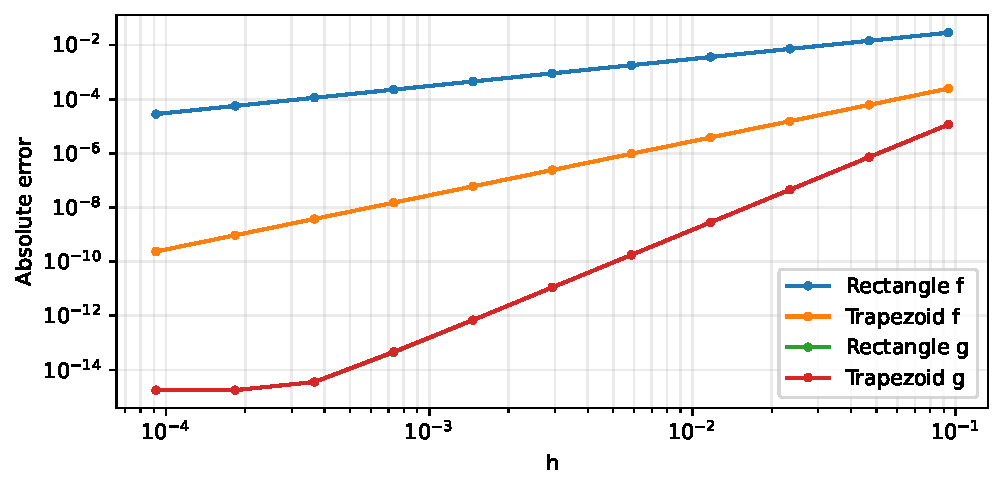
\includegraphics[width=.9\linewidth]{figures/assessments/ps2_quadrature.pdf}
\end{center}
上图的另外两条曲线对应下一题的 $g$. 数值证据与 Taylor/Euler--Maclaurin 给出的理论阶一致.
\end{solution}

\begin{exercise}\label{ps2-q4}
(原题 4, 1 分) 将第 3 题的函数改为 $g(x)=(x+1)^3(x-2)^2$, 在同一区间 $[-1,2]$ 重画收敛图. 两种方法现在各有几阶精度? (附加 1 分: 解释观察到的现象.)
\end{exercise}
\begin{solution}
实际两条误差曲线重合, 都为四阶. 由于 $g(-1)=g(2)=0$, $R_h=T_h$; 且 $g'(-1)=g'(2)=0$, 梯形的二阶主项消失. 用 Euler--Maclaurin 对五次多项式的精确有限展开,
\[
T_h-\int_{-1}^2g(x)\dd x
=\frac{h^2}{12}[g'(2)-g'(-1)]
-\frac{h^4}{720}[g'''(2)-g'''(-1)]= -\frac{3}{20}h^4.
\]
这里 $g'''(2)-g'''(-1)=108$; 后续项的端点导数差为零. 用 $t=x+1$ 积分 $t^3(t-3)^2$ 得真值 $3^6/60=12.15$. 拟合四阶曲线时须避开误差已接近机器精度的最细网格; 理论公式可直接核对每一行数值.
\end{solution}

\begin{exercise}\label{ps2-q5}
(原题 5, 3 分) 仍取 $f(x)=x/(1+x^4)$, 编写脚本实现一阶前向差分与二阶中心差分. 在间距 $h$ 的细网格上计算每个点的导数, 排除两个端点; 可沿用前题的网格约定.
\begin{enumerate}[label=\textbullet]
\item 求 $f'(1)$, 精确到小数点后 10 位.
\item 画截断误差关于 $h$ 的双对数图. 误差取所有内点上数值导数与精确导数之差的绝对值的最大值; 高精度数值导数也可代替精确值. 解释如何从图中看出收敛阶.
\end{enumerate}
\end{exercise}
\begin{solution}
解析微分得 $f'(x)=(1-3x^4)/(1+x^4)^2$, 故 $f'(1)=-0.5000000000$. 内点使用
$D_+f_j=(f_{j+1}-f_j)/h$,
$D_0f_j=(f_{j+1}-f_{j-1})/(2h)$, 与解析导数逐点比较.
一致 Taylor 估计分别给出 $O(h)$ 和 $O(h^2)$; 实际最大范数误差曲线的斜率约为 $1.000$ 和 $2.000$.
\begin{center}
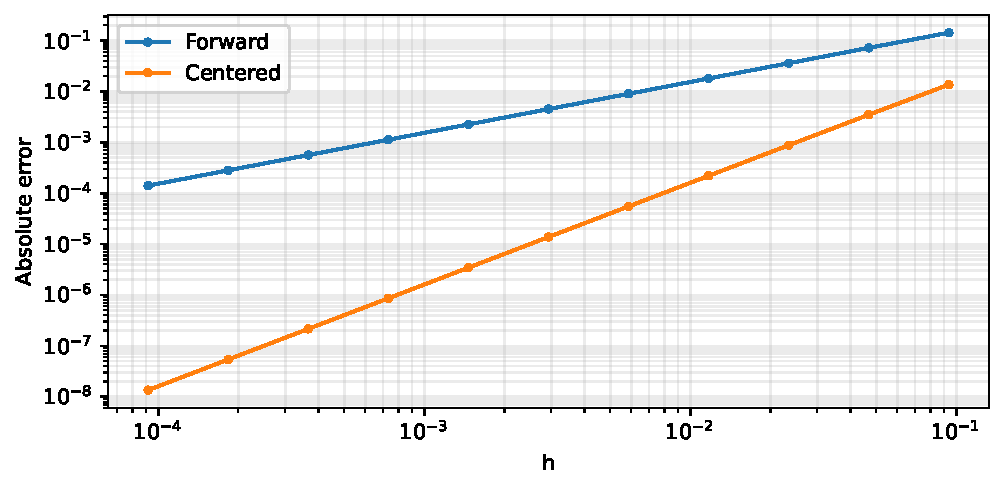
\includegraphics[width=.86\linewidth]{figures/assessments/ps2_differences.pdf}
\end{center}
源码以数组 \texttt{y[2:]-y[1:-1]} 和 \texttt{y[2:]-y[:-2]} 计算, 确保两种误差都只比较相同的内点.
\end{solution}

\originalchapter{作业 3}
MIT 18.330, Spring 2012. 原件: Homework 3, Due March 15. 以下解答均为 AI 编写, 非官方答案.

\begin{exercise}\label{ps3-q1}
(原题 1, 2.5 分) 通过对适当的插值多项式求导, 用 $f(0),f(h),f(2h)$ 设计 $f'(0)$ 的单边二阶差分公式; $0$ 是左端点. 用 Taylor 展开或课堂结果证明精度.
\end{exercise}
\begin{solution}
节点 $0,h,2h$ 的二次 Lagrange 插值多项式为
\[
p(x)=f(0)\frac{(x-h)(x-2h)}{2h^2}
-f(h)\frac{x(x-2h)}{h^2}+f(2h)\frac{x(x-h)}{2h^2}.
\]
求导后 $p'(0)=[-3f(0)+4f(h)-f(2h)]/(2h)$. 若 $f\in C^3$, 代入各节点的 Taylor 展开, 常数项及二阶项抵消, 得 $p'(0)=f'(0)-h^2f'''(0)/3+o(h^2)$, 因而是二阶单边公式.
\end{solution}

\begin{exercise}\label{ps3-q2}
(原题 2, 2.5 分) 考虑课堂上的 $[1\ 4\ 1]$ Simpson 公式
$\int_{-h}^h f(x)\dd x\simeq\frac h3[f(-h)+4f(0)+f(h)]$.
\begin{enumerate}[label=(\alph*)]
\item 虽然它由抛物线导出, 证明它对所有三次多项式仍精确.
\item 利用此结论证明, 若 $f\in C^4[-h,h]$, 则该积分的局部误差为 $O(h^5)$.
\end{enumerate}
原件补充: 积分四个节点的三次插值多项式得到另一种称为 $3/8$ 法的公式, 其局部误差也为 $O(h^5)$.
\end{exercise}
\begin{solution}
(a) 只需验证基 $1,x,x^2,x^3$: 公式分别给出 $2h,0,2h^3/3,0$, 与积分相同. 奇次项在对称区间及对称权重下都为零.
(b) 将 $f$ 分解为在 $0$ 处的三次 Taylor 多项式 $P_3$ 与余项 $r$, 若第四阶导数在一个固定邻域内有界, 则 $|r(x)|\le M|x|^4/24$. 公式对 $P_3$ 精确, 故总误差绝对值至多
\[
\int_{-h}^h|r(x)|\dd x+
\frac h3(|r(-h)|+4|r(0)|+|r(h)|)
\le \frac{Mh^5}{60}+\frac{Mh^5}{36}=\frac{2M}{45}h^5.
\]
该界不追求最优常数, 但已证明所需局部阶. 固定区间上的复合 Simpson 需再累计小区间数, 得全局四阶.
\end{solution}

\begin{exercise}\label{ps3-q3}
(原题 3, 2.5 分) 实现两端导数为零的夹持三次样条插值. 节点 $x_j=j$, $0\le j\le N$, 数据为
$y_0=1$, $y_1=0$, $y_k=1$ ($k\ge2$). 取 $N=10$, 在远比 10 个点更细的网格上画 $[x_0,x_{10}]$ 内的样条.
\end{exercise}
\begin{solution}
设 $M_j=s''(j)$. 节点处一阶导数连续及两端夹持条件给出三对角系统
\[
2M_0+M_1=6(y_1-y_0),\quad
M_{j-1}+4M_j+M_{j+1}=6(y_{j+1}-2y_j+y_{j-1}),\quad
M_9+2M_{10}=-6(y_{10}-y_9).
\]
中式取 $1\le j\le9$. 矩阵严格对角占优, 故可唯一解出 $M$. 对 $t=x-j\in[0,1]$,
\[
s_j(x)=\frac{M_j(1-t)^3+M_{j+1}t^3}{6}
+(y_j-M_j/6)(1-t)+(y_{j+1}-M_{j+1}/6)t.
\]
实验脚本显式组装并解该系统, 在 2001 个点上求值. 与 SciPy 的夹持样条独立实现比较, 最大差小于 $10^{-13}$, 两端导数均在舍入误差内为零. 图中的小幅振荡随远离凹陷节点快速衰减.
\begin{center}
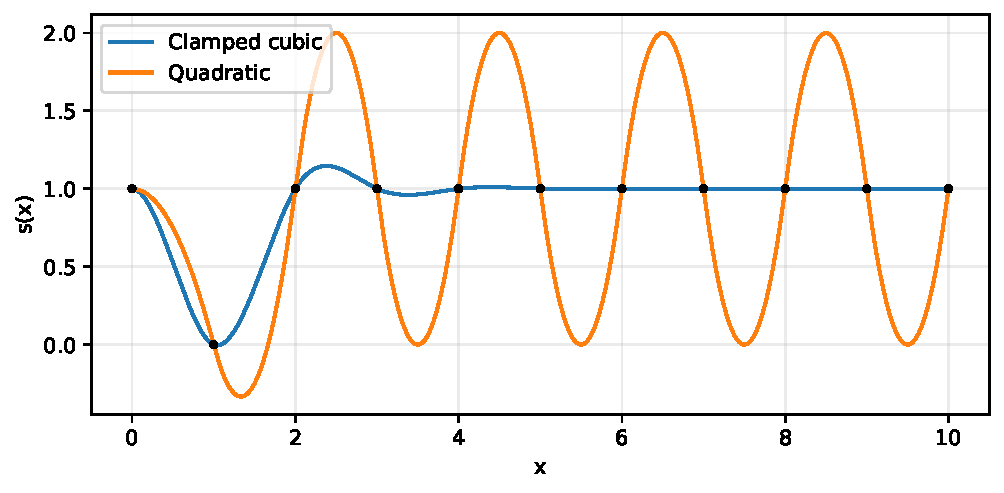
\includegraphics[width=.9\linewidth]{figures/assessments/ps3_splines.pdf}
\end{center}
图中三次样条和下一题的二次样条共用相同数据点与相同坐标轴, 便于比较.
\end{solution}

\begin{exercise}\label{ps3-q4}
(原题 4, 2.5 分) 二次样条是各段为二次多项式、节点处有一个连续导数的插值函数. 对数据 $\{x_j,y_j\}$, 在 $[x_j,x_{j+1}]$ 上为
\[
s_j(x)=y_j+z_j(x-x_j)+\frac{z_{j+1}-z_j}{2(x_{j+1}-x_j)}(x-x_j)^2,
\qquad z_{j+1}=-z_j+2\frac{y_{j+1}-y_j}{x_{j+1}-x_j}.
\]
插值与连续条件留下一个自由度 $z_0$, 以下取 $z_0=0$.
\begin{enumerate}[label=(\alph*)]
\item 对第 3 题数据计算 $z_j$, $1\le j\le10$.
\item 画 $[x_0,x_{10}]$ 上的二次样条.
\item 用一句话解释实际曲线拟合中二次样条为何不如线性和三次样条.
\end{enumerate}
\end{exercise}
\begin{solution}
(a) 依次得到 $(z_1,\ldots,z_{10})=(-2,4,-4,4,-4,4,-4,4,-4,4)$.
(b) 将这些斜率代入题给公式, 图见上一题的 Quadratic 曲线; 自 $j\ge2$ 起所有数据值虽为 $1$, 区间内部仍在 $0$ 与 $2$ 之间交替偏离.
(c) 二次样条的一阶导数连续约束通过 $z_{j+1}=-z_j+2\Delta y_j$ 传递不衰减的交替振荡, 对本类局部扰动既不如线性样条局部、也不如三次样条平滑稳定. 这解释本实验中的实用缺点, 不断言二次样条在每种用途上都较差.
\end{solution}

\originalchapter{作业 4}
MIT 18.330, Spring 2012. 原件: Homework 4, Due Tuesday April 3. 以下解答均为 AI 编写, 非官方答案.

\begin{exercise}\label{ps4-q1}
(原题 1, 1 分) 用 Newton 方法求 $3^{1/3}$, 达到 10 位精度, 并说明计算过程.
\end{exercise}
\begin{solution}
解 $f(x)=x^3-3=0$, 取 $x_0=1$, 迭代
$x_{k+1}=(2x_k+3/x_k^2)/3$. 前几项为
$1.6666666667$, $1.4711111111$, $1.4428120982$, $1.4422497896$,
$1.4422495703074416$. 下一步得到 $1.4422495703074085$, 残差约 $8.9\times10^{-16}$. 因此小数点后 10 位为 $1.4422495703$. 用 $f(1.4422495703)<0<f(1.44224957035)$ 及 $f'>0$ 可复核根的区间; 脚本保存实际迭代值.
\end{solution}

\begin{exercise}\label{ps4-q2}
(原题 2) 解 $x=\phi(x)$ 的一种方法是迭代 $x_{k+1}=\phi(x_k)$.
\begin{enumerate}[label=(\alph*)]
\item (1 分) 当 $\phi$ 为压缩映射, 即对所有 $x\ne y$ 有
$|\phi(x)-\phi(y)|<|x-y|$, 迭代收敛. 证明若对所有 $x$ 有 $|\phi'(x)|<1$, 则满足这个压缩性质.
\item (0.5 分) 找一个 $\phi$, 使固定点唯一, 但迭代发散.
\item (1 分) 设 $f$ 只有一个根 $x_*$, 且在根的邻域内 $f'\ne0$. 将 Newton 法写成固定点迭代, 用 (a) 给出一个关于 $f,f',f''$ 的邻域条件, 保证收敛到固定点.
\end{enumerate}
\end{exercise}
\begin{solution}
(a) 在定义域为区间且 $\phi$ 可微时, 中值定理给出
$|\phi(x)-\phi(y)|=|\phi'(\xi)||x-y|<|x-y|$.
整理注: 原题的逐对严格不等式比通常 Banach 压缩条件弱. Banach 定理的一种充分保证是不变的完整区间及统一常数 $q<1$, 不能仅凭逐点 $|\phi'|<1$ 断言任意起点收敛. 例如 $\phi(x)=\log(1+\ee^x)$ 的导数处处在 $(0,1)$ 内, 但没有实固定点.

(b) 取 $\phi(x)=2x$, 唯一固定点为 $0$; 任意 $x_0\ne0$ 的迭代为 $2^kx_0$, 故发散.

(c) $\phi(x)=x-f(x)/f'(x)$,
$\phi'(x)=f(x)f''(x)/[f'(x)]^2$. 充分条件是在闭区间
$I=[x_*-r,x_*+r]$ 上有 $f'\ne0$, $f\in C^2$, 且
$\sup_I|ff''/(f')^2|\le q<1$. 因 $\phi(x_*)=x_*$, 中值定理给出
$|\phi(x)-x_*|\le q|x-x_*|\le qr$, 所以 $\phi(I)\subset I$.
对 $x_0\in I$, 误差不超过 $q^k|x_0-x_*|$, 故迭代收敛.
\end{solution}

\begin{exercise}\label{ps4-q3}
(原题 3, 2.5 分) 用多变量 Newton 法求下列方程组的一个解:
\[
x_1^2+x_2^2+x_3^2=100,\qquad x_1x_2x_3=1,\qquad
x_1-x_2-\sin x_3=0.
\]
\end{exercise}
\begin{solution}
将三个左端减去右端组成 $G(x)$, Jacobian 为
\[
J(x)=\begin{pmatrix}
2x_1&2x_2&2x_3\\
x_2x_3&x_1x_3&x_1x_2\\
1&-1&-\cos x_3
\end{pmatrix}.
\]
每步解 $J(x_k)\Delta x=-G(x_k)$, 再取 $x_{k+1}=x_k+\Delta x$, 不显式求逆. 从 $(7,7,0.02)$ 出发实际得到
\[
(x_1,x_2,x_3)\approx
(7.081046012560867,\ 7.061047185906358,\ 0.02000015999317334).
\]
三方程残差最大绝对值小于 $2\times10^{-14}$. 题目只要求一个解; 该实验不主张方程组解唯一. 源码中的 \texttt{newton} 函数 保留各步残差.
\end{solution}

\begin{exercise}\label{ps4-q4}
(原题 4) 求 $F$ 极小值的 Newton 迭代为
$x_{k+1}=x_k-F'(x_k)/F''(x_k)$. 以下取
$F(x)=1+\int_0^x\arctan y\dd y$.
\begin{enumerate}[label=(\alph*)]
\item (0.5 分) 证明 $F''(x)>0$, 即 $F$ 严格凸. (原件附注: 严格凸函数总有唯一极小值.)
\item (0.5 分) 分别给出一个收敛的起点及一个发散的起点; 凸性不能保证 Newton 迭代收敛.
\item (1 分) 简述如何设计一个可靠方法, 在满足 $F'(a)<0$, $F'(b)>0$ 的区间 $[a,b]$ 中求凸函数的极小值.
\end{enumerate}
\end{exercise}
\begin{solution}
(a) $F'(x)=\arctan x$, $F''(x)=1/(1+x^2)>0$. 本题唯一极小点为 $0$, 极小值为 $1$. 整理注: 一般严格凸性只保证极小点至多一个, 不保证其存在, 如 $\ee^x$ 在 $\R$ 上没有最小点; 本题存在性由 $F'(0)=0$ 及导数变号给出.

(b) 迭代函数为 $\phi(x)=x-(1+x^2)\arctan x$. 取 $x_0=1/2$, 在 $|x|\le1/2$ 上
$|\phi'(x)|=2|x\arctan x|\le\arctan(1/2)<1$, 且 $\phi(0)=0$, 所以收敛.
取 $x_0=2$: 若 $x\ge2$, 令
$H(x)=(1+x^2)\arctan x-2x$; 有 $H(2)>0$,
$H'(x)=2x\arctan x-1>0$, 故 $\phi(x)<-x$.
$\phi$ 为奇函数, 所以迭代符号交替且绝对值严格增加. 若其绝对值有有限极限 $L\ge2$, 连续性将给出
$(1+L^2)\arctan L-L=L$, 与 $H(L)>0$ 矛盾; 故绝对值趋无穷.

(c) 对连续导数 $F'$ 二分. 在中点 $m$ 检查导数符号, 保留含零点的半区间; 区间长度每步减半. 凸性使 $F'$ 单调不减, 零点就是极小点; 若严格凸则极小点唯一. 也可加入受区间约束的 Newton 步, 但必须保留二分的收缩保证.
\end{solution}

\begin{exercise}\label{ps4-q5}
(原题 5, 2 分) 要精确测量电阻, 其标称值为 $R=2\Omega$. 接电池后用廉价万用表测得电压 $V=2.9\mathrm V$, 电流 $I=1.4\mathrm A$. 假定标称值和测量均有误差, 用 Newton 法最小化
\[
F(V,I,R)=(V-RI)^2+10(R-2)^2+10(V-2.9)^2+10(I-1.4)^2,
\]
求 $V,I,R$ 的“最佳”拟合.
\end{exercise}
\begin{solution}
令 $q=(V,I,R)^T$, $q_0=(2.9,1.4,2)^T$, $d=V-RI$,
$g=(1,-R,-I)^T$. 则
\[
\nabla F=2dg+20(q-q_0),\quad
\nabla^2F=2gg^T+20I_3+2d
\begin{pmatrix}0&0&0\\0&0&-1\\0&-1&0\end{pmatrix}.
\]
从 $q_0$ 出发每步解 Hessian 线性系统, 实际得到
\[
(V,I,R)\approx(2.894121035469170,\ 1.411806724241844,\ 2.008299961656205),
\quad F_{\min}\approx0.005884725643198.
\]
梯度最大绝对值约 $4.5\times10^{-15}$, Hessian 三个特征值约为 $19.9824,20.1123,33.9582$, 所以这是严格局部极小点.

还可验证全局最优性. $F$ 连续且由二次惩罚项控制, 当 $\|q\|\to\infty$ 时趋无穷, 故存在全局最小点. 因 $F(q_0)=0.01$, 每个全局最小点都落在
$|q_i-q_{0,i}|\le\sqrt{0.001}<0.032$ 的盒内. 该盒内
$|d|<0.25$, 故 Hessian 最小特征值至少为 $20-2|d|>19.5$ (秩一项半正定). 盒是凸集, $F$ 在盒内严格凸, 其中至多一个驻点. 实际找到的驻点在盒内, 因而必为唯一全局最小点.
\end{solution}

\originalchapter{作业 5}
MIT 18.330, Spring 2012. 原件: Homework 5, Due Tuesday April 12. 整理注: 原印星期与 2012 年 4 月 12 日 (星期四) 不符, 此处保留原件信息. 以下解答均为 AI 编写, 非官方答案.

\begin{exercise}\label{ps5-q1}
(原题 1, 4 分) 考虑简谐振动初值问题
$y''+\omega^2y=0$, $y(0)=y_0$, $y'(0)=y_1$.
以下取 $y_0=0$, $y_1=1$, $\omega=1$.
\begin{enumerate}[label=(\alph*)]
\item 显式求解.
\item 引入 $z=y'$, 将其写成两个一阶方程组成的系统.
\item 用前向 Euler 法数值求解. 找出保证稳定的时间步长条件, 在 $(y,z)$ 平面画出解曲线.
\item 对后向 Euler 法回答同样问题.
\item 对梯形法回答同样问题.
\item (附加 1 分) 严格解释为何梯形法的点“恰好”落在单位圆上.
\end{enumerate}
\end{exercise}
\begin{solution}
(a) $y(t)=\sin t$.
(b) $Y=(y,z)^T$ 满足 $Y'=AY$, $A=\left(\begin{smallmatrix}0&1\\-1&0\end{smallmatrix}\right)$, $Y(0)=(0,1)^T$.
(c) 前向法 $Y_{n+1}=(I+hA)Y_n$, 两个放大因子为 $1\pm\ii h$, 模为 $\sqrt{1+h^2}>1$. 因此没有正步长能使无限时间迭代有界; 半径每步乘以 $\sqrt{1+h^2}$, 向外螺旋. 对固定有限时间, 当 $h\to0$ 仍收敛, 这与绝对稳定区的判断不同.
(d) 后向法 $Y_{n+1}=(I-hA)^{-1}Y_n$, 放大因子模为 $1/\sqrt{1+h^2}<1$, 任意 $h>0$ 稳定, 但有人工阻尼.
(e) 梯形法 $Y_{n+1}=QY_n$, $Q=(I-hA/2)^{-1}(I+hA/2)$, 放大因子 $(1\pm\ii h/2)/(1\mp\ii h/2)$ 的模等于 $1$, 任意 $h>0$ 稳定.
(f) $A^T=-A$, 且各矩阵均为 $A$ 的有理函数, 彼此交换. 因此 $Q^TQ=I$, 即精确算术下 $\|Y_n\|_2=1$. 浮点计算只能达到舍入误差范围内的保持, 不保证字面上的完全相等.
\begin{center}
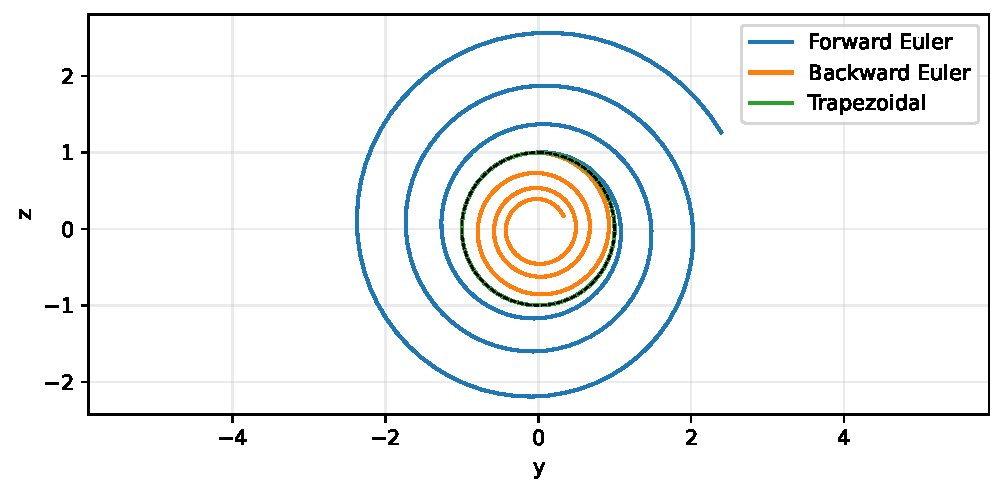
\includegraphics[width=.9\linewidth]{figures/assessments/ps5_phase.pdf}
\end{center}
实际取 $h=0.1$, 迭代 200 步; 前向、后向及梯形的最终半径分别为 $2.7048138294$, $0.3697112123$, $1.0000000000$. 梯形半径的最大偏差约 $8.3\times10^{-15}$.
\end{solution}

\begin{exercise}\label{ps5-q2}
(原题 2, 3 分) Leap-frog 法为
$y_{n+1}=y_{n-1}+2hf(t_n,y_n)$.
它是 $y'=f(t,y)$ 的最简单二步法. 求其在复数 $h\lambda$ 平面中的稳定区域.
\end{exercise}
\begin{solution}
对 $y'=\lambda y$, 设 $z=h\lambda$, 特征方程为
$r^2-2zr-1=0$. 两根的乘积为 $-1$, 若都在闭单位圆内, 则两根模都必须等于 $1$. 写 $r_1=\ee^{\ii\theta}$, 则 $r_2=-\ee^{-\ii\theta}$, 由和为 $2z$ 得 $z=\ii\sin\theta$. 因此只有虚轴线段可能稳定.
对 $z=\ii\eta$, $|\eta|<1$, 两根为
$\ii\eta\pm\sqrt{1-\eta^2}$, 模为 $1$ 且互异, 满足二步法根条件.
在端点 $\eta=\pm1$ 出现重根 $\pm\ii$, 通解含 $n(\pm\ii)^n$, 不稳定.
故按根条件稳定区域为 $\{\ii\eta: -1<\eta<1\}$, 包含 $0$, 没有二维内部. 若“绝对稳定”专指两根严格小于 $1$, 则该区域为空; 本题采用通常允许单位圆上单根的有界稳定定义.
\end{solution}

\begin{exercise}\label{ps5-q3}
(原题 3, 3 分) 考虑 $y'=-y^2$, $y(0)=100$, 真解为 $y(t)=1/(t+1/100)$.
\begin{enumerate}[label=(\alph*)]
\item 证明前向 Euler 迭代满足 $y_n\le100$.
\item 求保证前向 Euler 法稳定的步长条件, 并证明.
\item 对不同步长运行前向 Euler 法, 检查数值行为是否符合 (b) 的预期.
\item 再问 (原件再次标为 c)): 用显式法还是隐式法更好? 为什么?
\end{enumerate}
\end{exercise}
\begin{solution}
(a) $y_{n+1}=y_n-hy_n^2\le y_n$, 对任意 $h\ge0$ 归纳得 $y_n\le100$. 这个上界不保证下界或稳定.
(b) 若 $0<h\le1/100$, 则对 $0\le y_n\le100$,
$y_{n+1}=y_n(1-hy_n)\in[0,y_n]$, 所以解始终非负、有界; 在这一不变区间内迭代映射的导数 $1-2hy$ 属于 $[-1,1]$, 两条这样的轨迹之间的扰动不增长. 若 $h>1/100$, 首步变负. 写 $a_n=-y_n>0$, 后续有 $a_{n+1}=a_n+ha_n^2$. 若它有有限极限 $L$, 则 $L=L+hL^2$, 与 $L\ge a_1>0$ 矛盾, 故 $y_n\to-\infty$.
因此对给定初值, $0<h\le0.01$ 是轨迹有界的精确范围. 取等号时首步直接变成零, 虽有界却精度很差, 实用计算应取远小于 $0.01$ 的步长.

(c) 实验取 $h=0.005,0.01,0.015,0.02,0.021$. 前两者分别单调趋零、首步归零; 后三者首步为 $-50,-100,-110$, 随后发散, 与上述证明一致. 在真解附近仅考察 $|-2hy+1|\le1$ 并不足以保证数值轨迹留在真解的邻域.
\begin{center}
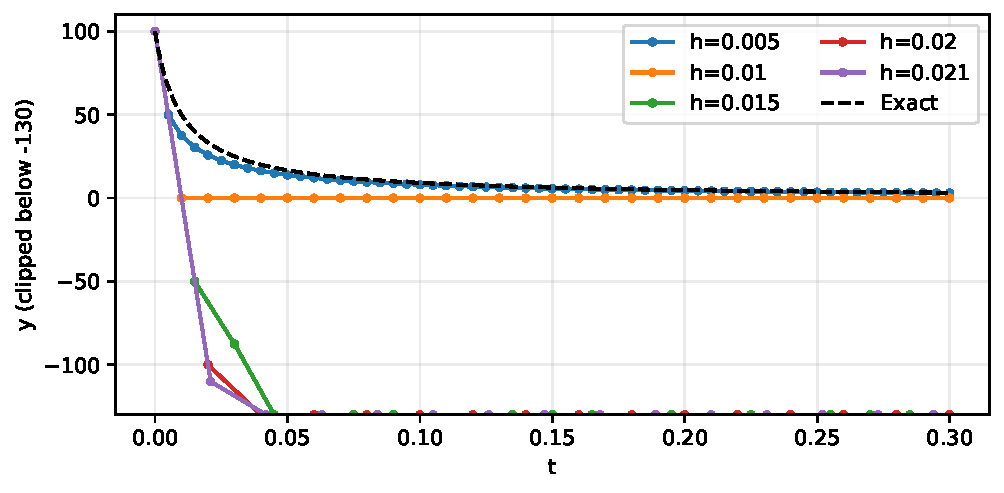
\includegraphics[width=.9\linewidth]{figures/assessments/ps5_nonlinear.pdf}
\end{center}
图对低于 $-130$ 的值作截断显示, 未将截断后的平台解释为稳定.

(原第二个 c)) 后向 Euler 满足 $hy_{n+1}^2+y_{n+1}-y_n=0$. 对非负 $y_n$ 选择正根, 用避免相消的形式
$y_{n+1}=2y_n/[1+\sqrt{1+4hy_n}]$,
任意 $h>0$ 都有 $0\le y_{n+1}\le y_n$, 且对输入的导数为
$1/(1+2hy_{n+1})\le1$. 隐式法允许较大步长而不出现负向爆破, 对稳定性更有利; 若要求准确解析初始快速变化, 两种法都仍需小步长或自适应. 本问题的隐式方程有显式正根公式, 每步代价也很小.
\end{solution}

\originalchapter{作业 6}
MIT 18.330, Spring 2012. 原件: Homework 6, Due Thursday April 26. 以下解答均为 AI 编写, 非官方答案.

\begin{exercise}\label{ps6-q1}
(原题 1, 7 分) 考虑混合 Neumann--Dirichlet 边值问题
$-u''=f$, $x\in[0,1]$, $u'(0)=0$, $u(1)=0$.
\begin{enumerate}[label=(\alph*)]
\item 求所有特征值 $\lambda_n$ 和特征函数 $v_n$, 使
$-v_n''=\lambda_nv_n$, $v_n'(0)=0$, $v_n(1)=0$.
手画前三个特征函数. 提示: 取正弦或余弦, 由边界条件确定.
\item 取 $x_j=jh$, $h=1/N$, $j=0,\ldots,N-1$, 用基本二阶差分离散二阶导数. 为简单起见, 将 Neumann 条件离散为 $(U_1-U_0)/h=0$.
写出离散系统的矩阵, 给出创建矩阵的 MATLAB 代码, 称它为 $T$.
\item 对适当的大 $N>100$, 用 MATLAB 的 \texttt{eig} 求 $T$ 的特征值与特征向量, 画前三个特征向量, 与连续预测比较. 提示: 特征值输出未必递增, 要同步排序特征值和特征向量.
\item 取 $f=1$, 离散成 $F_j=1$, 用 MATLAB 的反斜杠解 $TU=F$. 对不同 $N$ 绘制误差的双对数图, 误差取
$\|u-U\|_h=[h\sum_{j=0}^{N-1}(u(x_j)-U_j)^2]^{1/2}$.
提示: 可用很细网格的数值解作参考; 两网格应嵌套以便比较.
\item 原件称, 因边界条件仅一阶精度, 上述范数下局部截断误差为 $O(h)$. 要推出同一范数下全局误差也为 $O(h)$, $T$ 应满足什么性质?
\end{enumerate}
\end{exercise}
\begin{solution}
(a) 乘以 $v$ 并分部积分得 $\lambda\int_0^1v^2=\int_0^1(v')^2$, 因边界项为零, 非零特征函数不可能有 $\lambda\le0$ (等号会使 $v$ 为常数再由右端值为零排除).
因此 $v=A\cos(\sqrt\lambda x)+B\sin(\sqrt\lambda x)$, 左端导数条件给出 $B=0$, 右端给出
$\sqrt\lambda=(n+1/2)\pi$, $n=0,1,\ldots$.
于是 $\lambda_n=(n+1/2)^2\pi^2$, $v_n(x)=\cos((n+1/2)\pi x)$, 可乘任意非零常数. 下图虚线即前三个余弦, 依次有零、一、两个内部零点.

(b) 整理注: 若保留边界方程的一整行, 其右端必须是 $0$, 不能在该行也取 $F_0=1$; 而对包含边界行的矩阵直接用普通 \texttt{eig} 比较微分算子谱, 结果会依赖边界行的缩放. 为同时明确 (c)、(d), 本解答先消去 $U_0=U_1$, 将独立未知量取为
$W=(U_1,\ldots,U_{N-1})^T$, 并将所得矩阵称为 $T$. 最后恢复 $U_0=U_1$. 这保留全部题给网格点和边界条件, 不在边界处额外施加 $-u''=f$.
\[
T=\frac1{h^2}\begin{pmatrix}
1&-1&&\\
-1&2&-1&\\
&\ddots&\ddots&\ddots\\
&&-1&2
\end{pmatrix}_{(N-1)\times(N-1)}.
\]
完整未消元系统的第一行为 $(-U_0+U_1)/h=0$, 其余行为 $(-U_{j-1}+2U_j-U_{j+1})/h^2=F_j$, $1\le j\le N-1$, 最后一行代入 $U_N=0$. MATLAB 核心代码为
\begin{verbatim}
h=1/N; m=N-1;
T=diag(2*ones(m,1))+diag(-ones(m-1,1),1) ...
  +diag(-ones(m-1,1),-1);
T(1,1)=1; T=T/h^2;
[V,D]=eig(T); [lam,idx]=sort(diag(D)); V=V(:,idx);
W=T\ones(m,1); U=[W(1);W];
\end{verbatim}

(c) 对 $m=N-1$, 特征向量在独立节点上可取
$w_j=\cos((j-1/2)\theta)$, $1\le j\le m$;
左端虚拟值 $w_0=w_1$, 右端 $w_{m+1}=0$, 故
$\theta_n=(n+1/2)\pi/(N-1/2)$,
$\lambda_{n,h}=4h^{-2}\sin^2(\theta_n/2)$, $0\le n\le N-2$.
当 $h\to0$ 时固定编号的特征值趋向 (a) 的值.
实际取 $N=256$, 前三个为 $2.4770598945,22.2929773029,61.9218162242$, 连续值为
$2.4674011003,22.2066099025,61.6850275068$.
\begin{center}
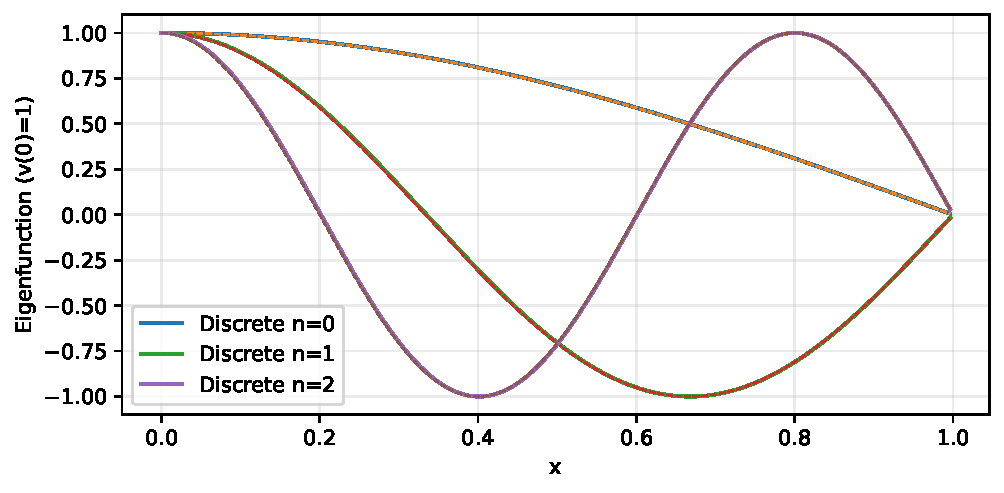
\includegraphics[width=.88\linewidth]{figures/assessments/ps6_eigenvectors.pdf}
\end{center}
脚本同步取前三个递增特征值及对应向量, 恢复 $U_0=U_1$, 并归一化左端值为 $1$. 实际 Python 使用对称三对角特征求解器; 上述 MATLAB 代码给出题目要求的 \texttt{eig} 等价做法.

(d) 真解为 $u(x)=(1-x^2)/2$. 消元系统的各内部右端确为 $1$, 可直接解析核对
$U_j=(1-x_j^2)/2-(h/2)(1-x_j)$, $0\le j\le N$, 它满足 $U_0=U_1$, $U_N=0$ 和所有内部差分方程. 因而
\[
\|u-U\|_h=\frac h2\left[h\sum_{j=0}^{N-1}(1-jh)^2\right]^{1/2}
\sim\frac{h}{2\sqrt3}.
\]
实际 $N=16,32,\ldots,4096$ 的误差拟合斜率约 $1.001$, 与一阶一致. 采用解析真解避免参考网格误差污染.
\begin{center}
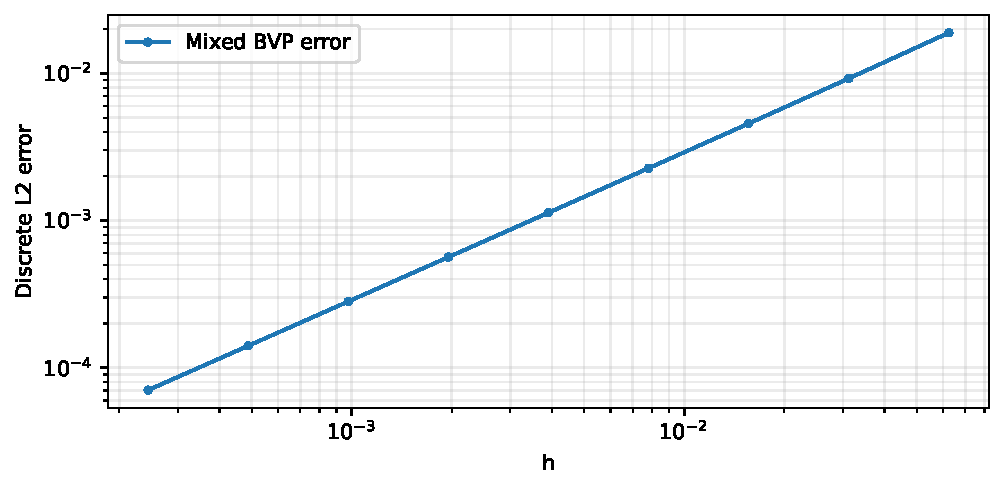
\includegraphics[width=.85\linewidth]{figures/assessments/ps6_convergence.pdf}
\end{center}

(e) 一般若 $\tau=T u_{\mathrm{grid}}-F$, $e=u_{\mathrm{grid}}-U$, 则 $Te=\tau$. 从 $\|\tau\|_h=O(h)$ 推出同阶全局误差的充分性质是稳定性: 诱导范数 $\|T^{-1}\|_{h\to h}\le C$ 一致于 $h$.
对本题对称正定的消元矩阵, 该范数等于 $1/\lambda_{0,h}$, 由 (c) 的公式有统一正下界 (例如 $\lambda_{0,h}\ge1$), 所以一致有界.

但原件“局部截断误差在同一二次范数中为 $O(h)$”并未随边界方程形式自动成立. 对 (b) 的明确消元约定和本题二次真解, $\tau=(1/2,0,\ldots,0)^T$, 在内部节点范数中是 $\sqrt h/2=O(h^{1/2})$. 单纯范数估计只给 $O(h^{1/2})$, 不能由它假证一阶. 实际
$(T^{-1}e_1)_j=h(1-x_j)$, 直接给出 (d) 的 $O(h)$ 全局误差; 恢复边界点后仍同阶. 因此保留原问并回答其所需的稳定性质, 同时明确原件关于局部范数的不足, 不把不同边界行缩放混成一个无条件结论.
\end{solution}

\begin{exercise}\label{ps6-q2}
(原题 2, 2 分) 考虑 Neumann 问题
$-\frac{\dd}{\dd x}[(1+x^2)u']=f$,
$x\in[0,1]$, $u'(0)=u'(1)=0$.
\begin{enumerate}[label=(\alph*)]
\item 证明 $f=1$ 时无解. 提示: 两端积分.
\item 求一个保证存在解的 $f$ 的条件.
\end{enumerate}
\end{exercise}
\begin{solution}
(a) 积分左端为 $-[(1+x^2)u']_0^1=0$, 右端为 $1$, 矛盾.
(b) 对连续 $f$, 充要条件为 $\int_0^1f(x)\dd x=0$.
必要性同 (a). 若满足条件, 令
$u'(x)=-[\int_0^x f(t)\dd t]/(1+x^2)$, 再取
\[
u(x)=C-\int_0^x\frac{\int_0^s f(t)\dd t}{1+s^2}\dd s.
\]
则 $u\in C^2$, 两端导数为零, 并满足微分方程. 常数 $C$ 任意, 体现纯 Neumann 问题的非唯一性.
\end{solution}

\begin{exercise}\label{ps6-q3}
(原题 3, 1 分) 设 $A=\left(\begin{smallmatrix}2&a\\1&0\end{smallmatrix}\right)$.
\begin{enumerate}[label=(\alph*)]
\item 对哪些 $a$ 可逆?
\item 不计算特征值和特征向量, 求使 $A$ 存在特征向量的标准正交基的 $a$, 并解释.
\end{enumerate}
\end{exercise}
\begin{solution}
(a) $\det A=-a$, 故当且仅当 $a\ne0$ 可逆.
(b) 对实标准正交特征基, $A=QDQ^T$ 必为对称矩阵, 所以 $a=1$ 是必要条件; 此时矩阵实对称, 由谱定理也充分.
若允许复正交基, 矩阵必须正规; 比较 $AA^*$ 与 $A^*A$ 的非对角元同样给出 $2=2a$, 仍只有 $a=1$.
\end{solution}

\originalchapter{作业 7}
MIT 18.330, Spring 2012. 原件: Homework 7, Due Thursday May 3. 以下解答均为 AI 编写, 非官方答案. 本章使用
$\widehat f(k)=\int_\R f(x)\ee^{-\ii kx}\dd x$,
$f(x)=(2\pi)^{-1}\int_\R\widehat f(k)\ee^{\ii kx}\dd k$ 的约定.

\begin{exercise}\label{ps7-q1}
(原题 1, 3 分) 证明 Fourier 变换的下列性质 ($x,k\in\R$):
\begin{enumerate}[label=(\alph*)]
\item 缩放: 若 $g(x)=f(x/a)$, $a>0$, 则 $\widehat g(k)=a\widehat f(ak)$.
\item 共轭: 若 $g(x)=\overline{f(x)}$, 则 $\widehat g(k)=\overline{\widehat f(-k)}$.
\item 对称性: 若 $f$ 实值且为偶函数 ($f(x)=f(-x)$), 则 $\widehat f$ 也实值且为偶函数.
\item 对称性: 若 $f$ 实值且为奇函数 (原件括号却印为 $f(x)=f(-x)$), 证明 $\widehat f$ 纯虚且为奇函数.
\end{enumerate}
\end{exercise}
\begin{solution}
以 $f\in L^1(\R)$ 为足以保证各积分存在的条件.
(a) 代换 $x=ay$, $\dd x=a\dd y$, 得
$\widehat g(k)=a\int_\R f(y)\ee^{-\ii(ak)y}\dd y=a\widehat f(ak)$.
(b) 对积分取共轭,
$\widehat g(k)=\overline{\int_\R f(x)\ee^{\ii kx}\dd x}=\overline{\widehat f(-k)}$.
(c) 分解为余弦和正弦积分; $f(x)\sin(kx)$ 为奇函数, 其积分为零, 所余余弦积分实值且关于 $k$ 为偶.
(d) 整理注: 按“奇函数”将括号修为 $f(-x)=-f(x)$. 此时 $f(x)\cos(kx)$ 为奇函数, 故余弦积分消失;
$\widehat f(k)=-\ii\int_\R f(x)\sin(kx)\dd x$, 它纯虚且关于 $k$ 为奇. 若同时照抄括号的偶条件与文字的奇条件, 只剩 $f=0$, 不能代表原问意图.
\end{solution}

\begin{exercise}\label{ps7-q2}
(原题 2, 3 分) 定义 $\operatorname{sinc}(x)=\sin x/x$, $x=0$ 处以连续延拓取值 $1$.
\begin{enumerate}[label=(\alph*)]
\item 证明 sinc 不可积, 即不属于 $L^1(\R)$. 提示: 若 $f\ge g\ge0$ 且 $\int g$ 发散, 则 $\int f$ 也发散.
\item 含 sinc 的某些积分仍有意义. 根据 Fourier 变换理论预测 $\int_{-\infty}^{\infty}\operatorname{sinc}(x)\dd x$ 的值.
\end{enumerate}
\end{exercise}
\begin{solution}
(a) 在 $I_n=[n\pi+\pi/6,n\pi+5\pi/6]$ ($n\ge1$) 上,
$|\sin x|\ge1/2$, $x\le(n+1)\pi$, 故
$\int_{I_n}|\sin x/x|\dd x\ge1/[3(n+1)]$.
对互不重叠的这些区间求和得到发散的调和下界, 因而 $\int_\R|\operatorname{sinc}x|\dd x=\infty$.
(b) 区间指示函数 $\mathbf1_{[-1,1]}(k)$ 的逆变换为
$(2\pi)^{-1}\int_{-1}^1\ee^{\ii kx}\dd k=\sin x/(\pi x)$.
因此在广义 Fourier 意义下 $\widehat{\operatorname{sinc}}=\pi\mathbf1_{[-1,1]}$, 零频率对应积分 $\pi$.
普通反常积分也确实存在: 在 $[A,B]$ 对 $\sin x/x$ 分部积分, 尾部绝对值不超过 $3/A$, 从而满足 Cauchy 条件.
为核对常数, 对 $\epsilon>0$ 有
$\int_0^\infty \ee^{-\epsilon x}\sin x/x\dd x=\arctan(1/\epsilon)$: 将 $\sin x$ 换成 $\sin(bx)$ 后对 $b$ 求导, 得 $\epsilon/(\epsilon^2+b^2)$, 从 $b=0$ 积至 $1$.
分部积分给出对 $\epsilon\ge0$ 一致的 $O(1/A)$ 尾界, 故可先控尾再令 $\epsilon\downarrow0$, 得半轴积分为 $\pi/2$. sinc 为偶函数, 双半轴反常积分为 $\pi$, 并非绝对收敛的 Lebesgue 积分.
\end{solution}

\begin{exercise}\label{ps7-q3}
(原题 3, 2 分) 设核 $K(x)$, 考虑积分方程
\[
u(x)+\int_{-\infty}^{\infty}K(x-y)u(y)\dd y=f(x).
\]
类似方程出现于计算机图形渲染以及雷达波被飞机散射等问题. 用 Fourier 变换给出 $u$ 的公式. $K$ 满足何种条件可避免除零?
\end{exercise}
\begin{solution}
积分项为卷积 $K*u$, 变换后
$(1+\widehat K(k))\widehat u(k)=\widehat f(k)$.
只要 $1+\widehat K(k)\ne0$, 形式上
\[
u(x)=\frac1{2\pi}\int_\R
\frac{\widehat f(k)}{1+\widehat K(k)}\ee^{\ii kx}\dd k.
\]
整理注: 点态不为零仅避免逐点除零, 还不足以保证任意 $L^2$ 右端的稳定求解. 一个常用充分条件是 $K\in L^1(\R)$ 且
$\inf_{k\in\R}|1+\widehat K(k)|\ge c>0$; 则该乘子在 $L^2$ 上有界可逆, 公式按 $L^2$ 逆变换理解. 例如 $\|K\|_1<1$ 即足够, 因 $|\widehat K|\le\|K\|_1$. 对更强的点态积分公式, 还需被积函数可积等额外条件.
\end{solution}

\begin{exercise}\label{ps7-q4}
(原题 4, 2 分) 证明 $v_k(x)=c\ee^{-\ii kx}$ ($k\in\Z$) 在 $[0,2\pi]$ 上关于内积
$\langle f,g\rangle=\int_0^{2\pi}f(x)\overline{g(x)}\dd x$ 正交, 并求使其规范化的 $c$.
\end{exercise}
\begin{solution}
对 $k\ne\ell$,
$\langle v_k,v_\ell\rangle=|c|^2[\ee^{\ii(\ell-k)x}/(\ii(\ell-k))]_0^{2\pi}=0$;
对 $k=\ell$ 内积为 $2\pi|c|^2$. 所以通常取正实常数 $c=1/\sqrt{2\pi}$; 任意模为该值的复数也可以. 原件内积中的共轭线与 (b) 的共轭线均按实际 PDF 核对保留, 不按丢失共轭的文本提取结果改题.
\end{solution}

\originalchapter{作业 8}
MIT 18.330, Spring 2012. 原件: Homework 8, Not due; Fourier exercises (05/15). 本份为不需提交的练习, 原件各题均无分值. 以下解答均为 AI 编写, 非官方答案.

\begin{exercise}\label{ps8-q1}
(原题 1) 证明 $C^p$ 周期函数 ($p\ge1$) 的 Fourier 级数系数按 $|k|^{-p}$ 衰减.
\end{exercise}
\begin{solution}
取周期 $2\pi$, $c_k=(2\pi)^{-1}\int_0^{2\pi}f(x)\ee^{-\ii kx}\dd x$; 一般周期只改变常数. 对非零 $k$ 分部积分 $p$ 次, 因函数及其前 $p-1$ 阶导数在两端衔接, 每次边界项均为零, 故
\[
c_k=\frac1{(\ii k)^p}\frac1{2\pi}
\int_0^{2\pi}f^{(p)}(x)\ee^{-\ii kx}\dd x,
\qquad |c_k|\le\frac{\|f^{(p)}\|_{L^1}}{2\pi|k|^p}.
\]
这里 $p$ 为整数; $C^p$ 是周期意义下的光滑性, 不是仅在闭区间内部有 $p$ 阶导数. 对 $k=0$ 不作衰减断言.
\end{solution}

\begin{exercise}\label{ps8-q2}
(原题 2) 证明用梯形法积分 $C^p$ 周期函数的误差为 $O(h^p)$.
\end{exercise}
\begin{solution}
设 $h=2\pi/L$, 周期梯形法为 $Q_h=h\sum_{j=0}^{L-1}f(jh)$, 两端不重复.
当 $p\ge2$ 时, 上题的系数绝对可和, 可逐项代入求和. 根单位恒等式给出
$Q_h=2\pi\sum_{\ell\in\Z}c_{\ell L}$, 而真积分为 $2\pi c_0$.
于是 $|Q_h-\int f|\le C L^{-p}\sum_{\ell\ne0}|\ell|^{-p}=O(h^p)$.

当 $p=1$ 时, 不能引用发散的 $\sum |\ell|^{-1}$ 作上界. 直接逐格比较: $f\in C^1$ 有 $|f(x)-f(jh)|\le\|f'\|_\infty h$,
每格积分误差至多 $\|f'\|_\infty h^2/2$, 共 $L$ 格, 所以误差 $O(h)$, 完成端点情形. 非周期函数端点未衔接时, 此谱收敛推理不适用.
\end{solution}

\begin{exercise}\label{ps8-q3}
(原题 3) 证明 $C^p$ 周期函数的带限微分的 $L^2$ 误差为 $O(h^{p-3/2})$.
\end{exercise}
\begin{solution}
明确采用等距采样后的三角插值微分. 取奇数点数 $L=2M+1$, $h=2\pi/L$, 以免偶数网格的 Nyquist 单模约定影响陈述. 设连续 Fourier 系数为 $c_k$, 插值系数为
$a_k=\sum_{\ell\in\Z}c_{k+\ell L}$ ($|k|\le M$).
带限微分为 $D_hf=\sum_{|k|\le M}\ii k a_k\ee^{\ii kx}$.
当 $p\ge2$ 时绝对求和合法, 上题的衰减估计给出
$|a_k-c_k|\le C L^{-p}$, 因 $|k+\ell L|\ge (|\ell|-1/2)L$.
由 Parseval,
\[
\begin{split}
\|f'-D_hf\|_2^2
&=2\pi\sum_{|k|>M}k^2|c_k|^2
+2\pi\sum_{|k|\le M}k^2|a_k-c_k|^2\\
&\le C\sum_{k>M}k^{2-2p}+CL^{-2p}\sum_{|k|\le M}k^2
\le C M^{3-2p}.
\end{split}
\]
开方后即 $O(h^{p-3/2})$. 第一项为截断误差, 第二项为混叠误差; 若采用最佳带限投影后求导, 只需第一项.

整理注: 对 $p=1$ 题给幂为 $h^{-1/2}$, 并不保证误差趋零. 此时可用 $f\in H^1$ 的更强信息证明 $\|f'-D_hf\|_2=O(1)$, 从而也满足原问的较弱界. 具体地, $\sum n^2|c_n|^2<\infty$ 还保证 $\sum |c_n|<\infty$, 混叠式仍合法. 对 $|k|\le M$ 的非主频项, Cauchy--Schwarz 给出
\[
|a_k-c_k|^2\le
\left(\sum_{\ell\ne0}|k+\ell L|^2|c_{k+\ell L}|^2\right)
\left(\sum_{\ell\ne0}|k+\ell L|^{-2}\right),
\]
第二因子至多 $C/L^2$, 再乘 $k^2\le M^2$ 并对 $k$ 求和, 得不超过 $C\sum n^2|c_n|^2$, 与高频尾项一同给出一致有界性. 不能用不收敛的 $\sum k^0$ 假证 $p=1$ 的速率.
\end{solution}

\begin{exercise}\label{ps8-q4}
(原题 4) 设 $f(x)=1/(1+x^2)$, 已知 $\widehat f(k)=\pi\ee^{-|k|}$. 本题在全实线上讨论 $x,k\in\R$, 没有边界.
\begin{enumerate}[label=\textbullet]
\item 求最佳带限逼近 $f_N$ (其 Fourier 变换支撑于 $[-N,N]$) 的误差 $\|f-f_N\|_2$ 关于 $N$ 的衰减率.
\item 对样本 $x_j=jh$ 的带限插值 $p_h$, 求 $\|f-p_h\|_2$ 关于 $h$ 的衰减率.
\item 同样求带限微分误差及梯形法误差的衰减率.
\end{enumerate}
\end{exercise}
\begin{solution}
第一项. $L^2$ 最佳逼近是 Fourier 变换截断:
$\widehat f_N=\widehat f\mathbf1_{[-N,N]}$. 由 Plancherel,
\[
\|f-f_N\|_2^2=\frac1{2\pi}\int_{|k|>N}\pi^2\ee^{-2|k|}\dd k
=\frac\pi2\ee^{-2N},\qquad
\|f-f_N\|_2=\sqrt{\pi/2}\ee^{-N}.
\]

第二项. 令 $K=\pi/h$, 带限插值采用 sinc 采样重建
$p_h(x)=\sum_{j\in\Z} f(jh)\operatorname{sinc}(\pi(x/h-j))$.
其变换在 $|k|\le K$ 上等于 $\sum_{\ell\in\Z}\widehat f(k+2K\ell)$, 区间外为零. 本题衰减足够快, 泊松求和与重建均可应用. 在主带内的混叠量恰为
\[
A(k)=\frac{2\pi\ee^{-2K}}{1-\ee^{-2K}}\cosh k.
\]
带外误差与带内混叠支撑互不相交, 所以
\[
\|f-p_h\|_2^2=\frac\pi2\ee^{-2K}
+\frac{2\pi\ee^{-4K}}{(1-\ee^{-2K})^2}
\left(K+\frac{\sinh2K}{2}\right)
\sim\pi\ee^{-2K}.
\]
故 $\|f-p_h\|_2\sim\sqrt\pi\ee^{-\pi/h}$, 即指数衰减, 不能把混叠误差当作零.

第三项的微分. 将上述两段变换误差各乘 $\ii k$. 带外平方误差为
\[
\pi\int_K^\infty k^2\ee^{-2k}\dd k
=\pi\ee^{-2K}\left(\frac{K^2}{2}+\frac K2+\frac14\right).
\]
带内平方误差为 $(2\pi)^{-1}\int_{-K}^Kk^2A(k)^2\dd k$, 渐近等于 $(\pi/2)K^2\ee^{-2K}$; 可由 $\cosh^2k=(1+\cosh2k)/2$ 积分或分部积分得到. 合并后
$\|f'-p_h'\|_2\sim\sqrt\pi K\ee^{-K}$,
即 $\Theta(h^{-1}\ee^{-\pi/h})$. 若只求最佳投影的导数, 常数变为 $\sqrt{\pi/2}$, 指数和多项式因子相同.

第三项的求积. 无边界梯形法为 $Q_h=h\sum_{j\in\Z}f(jh)$, 真积分为 $\widehat f(0)=\pi$. 泊松求和给出
\[
Q_h=\sum_{\ell\in\Z}\pi\ee^{-|2\pi\ell/h|}
=\pi+\frac{2\pi}{\ee^{2\pi/h}-1}.
\]
因此求积误差为 $\Theta(\ee^{-2\pi/h})$, 比插值误差的指数更快. 这是零频率混叠量的特性, 不能把所有谱方法误差都写成同一个指数.
\end{solution}

\begin{exercise}\label{ps8-q5}
(原题 5) 陈述并证明离散卷积定理.
\end{exercise}
\begin{solution}
先固定归一化约定. 对长度 $L$ 的周期序列,
$\widehat a_k=\sum_{j=0}^{L-1}a_j\ee^{-2\pi\ii jk/L}$,
$a_j=L^{-1}\sum_{k=0}^{L-1}\widehat a_k\ee^{2\pi\ii jk/L}$.
循环卷积定义为 $(a*b)_j=\sum_{m=0}^{L-1}a_m b_{(j-m)\bmod L}$.
定理是 $\widehat{a*b}_k=\widehat a_k\widehat b_k$.
证明仅需有限和换序及换元 $r=(j-m)\bmod L$:
\[
\begin{split}
\widehat{a*b}_k
&=\sum_{m=0}^{L-1}a_m\sum_{j=0}^{L-1}b_{j-m}\ee^{-2\pi\ii jk/L}\\
&=\left(\sum_m a_m\ee^{-2\pi\ii mk/L}\right)
\left(\sum_r b_r\ee^{-2\pi\ii rk/L}\right).
\end{split}
\]
每个求和指标均按模 $L$ 解释, 指数的周期性保证换元合法. 同理点乘对应
$\widehat{ab}_k=L^{-1}\sum_m\widehat a_m\widehat b_{k-m}$.
若改用带 $1/L$ 的卷积或其他 DFT 归一化, 常数必须相应改变; 非循环线性卷积需先补零, 避免绕回混叠.
\end{solution}

\begin{thebibliography}{9}
\bibitem{mitcourse} Laurent Demanet. \textit{18.330 Introduction to Numerical Analysis, Spring 2012}. Massachusetts Institute of Technology, MIT OpenCourseWare. \href{https://ocw.mit.edu/courses/18-330-introduction-to-numerical-analysis-spring-2012/pages/lecture-notes/}{官方七章讲义目录}. 原始 PDF 的直链、页数和 SHA-256 见随附 source-manifest.json.
\bibitem{tao} Terence Tao. \textit{Analysis I}. 原讲义第 1 章推荐的分析参考书; 原件未指明所用版次.
\bibitem{dahlquist} Germund Dahlquist, Åke Björck. \textit{Numerical Methods}. 原讲义第 1 章推荐的数值方法参考书; 原件未指明所用版次.
\bibitem{trefethen} Lloyd N. Trefethen. \textit{Spectral Methods in MATLAB}. SIAM, Philadelphia, 2000. \href{https://people.maths.ox.ac.uk/trefethen/spectral.html}{作者提供的书目与程序页面}. 本书正文中第 30, 43, 44, 47 页等定位沿用原讲义的引用.
\bibitem{sulimayers} Endre Süli, David F. Mayers. \textit{An Introduction to Numerical Analysis}. Cambridge University Press, 2003. \href{https://doi.org/10.1017/CBO9780511801181}{出版社书目}. 例 6.1, 第 6 章及第 311, 351 页等定位沿用原讲义.
\end{thebibliography}
\end{document}
